\documentclass[12pt,a4paper]{report}

% --- Gói ngôn ngữ và mã hóa tiếng Việt ---
\usepackage[utf8]{inputenc}
\usepackage[vietnamese]{babel}
\usepackage[T5]{fontenc}

% --- Canh lề và định dạng trang ---
\usepackage[top=2.5cm, bottom=2.5cm, left=3cm, right=2cm]{geometry}
\usepackage{fancyhdr}
\setlength{\headheight}{15pt}
\usepackage{titlesec}

% --- Bảng, hình ảnh, toán học và ký hiệu ---
\usepackage{amsmath, amssymb}
\usepackage{graphicx}
\usepackage{booktabs}
\usepackage{tabularx}
\usepackage{longtable}
\usepackage{float}
\usepackage{caption}
\usepackage{subcaption}

% --- Định dạng code mã nguồn ---
\usepackage{listings}
\usepackage{xcolor}

\definecolor{codegreen}{rgb}{0.13,0.55,0.13}
\definecolor{codegray}{rgb}{0.5,0.5,0.5}
\definecolor{codepurple}{rgb}{0.58,0,0.82}
\definecolor{backcolour}{rgb}{0.96,0.97,0.98}

\lstdefinestyle{mystyle}{
    backgroundcolor=\color{backcolour},   
    commentstyle=\color{codegreen},
    keywordstyle=\color{blue}\bfseries,
    numberstyle=\tiny\color{codegray},
    stringstyle=\color{codepurple},
    basicstyle=\ttfamily\footnotesize,
    breakatwhitespace=false,         
    breaklines=true,                 
    captionpos=b,                    
    keepspaces=true,                 
    numbers=left,                    
    numbersep=5pt,                  
    showspaces=false,                
    showstringspaces=false,
    showtabs=false,                  
    tabsize=2
}
\lstset{style=mystyle}

% --- Liên kết và màu sắc tài liệu ---
\usepackage{hyperref}
\hypersetup{
    colorlinks=true,
    linkcolor=blue!70!black,
    filecolor=magenta,      
    urlcolor=cyan!70!black,
    citecolor=green!50!black,
    plainpages=false,
    pdfpagelabels=true,
    pdftitle={Báo cáo dự án IoT: FloodGuard - Hệ thống chống ngập tự động},
    pdfauthor={Vũ Minh Quân, Nguyễn Đức Huy, Phạm Đức Mạnh},
}

% --- Header và Footer ---
\pagestyle{fancy}
\fancyhf{}
\fancyhead[L]{\small\slshape FloodGuard - Hệ Thống Chống Ngập Tự Động}
\fancyhead[R]{\small\slshape ESP32 IoT Project}
\fancyfoot[C]{\thepage}
\renewcommand{\headrulewidth}{0.4pt}
\renewcommand{\footrulewidth}{0.4pt}

% ==================== BẮT ĐẦU TÀI LIỆU ====================
\begin{document}

\pagenumbering{alph}

% --- TRANG BÌA ---
% Khung viền đôi trang bìa chuẩn luận văn: Khung đậm dày ở ngoài và khung mỏng nhỏ hơn ở trong
\AddToHookNext{shipout/background}{%
    % Khung ngoài: Nét đậm dày (2.8pt)
    % Tọa độ chuẩn: Trái 25mm, Phải 15mm (Rộng 170mm), Trên 16mm, Dưới 16mm (Cao 265mm)
    \put(70.87,-48.15){\rule{481.89pt}{2.8pt}}% Cạnh trên ngoài
    \put(70.87,-796.54){\rule{481.89pt}{2.8pt}}% Cạnh dưới ngoài
    \put(70.87,-796.54){\rule{2.8pt}{751.18pt}}% Cạnh trái ngoài
    \put(549.96,-796.54){\rule{2.8pt}{751.18pt}}% Cạnh phải ngoài
    %
    % Khung trong: Nét thanh mỏng (0.9pt), lùi vào trong 2.5mm so với khung ngoài
    % Trái 27.5mm (Rộng 165mm), Trên 18.5mm (Cao 260mm)
    \put(77.95,-53.34){\rule{467.72pt}{0.9pt}}% Cạnh trên trong
    \put(77.95,-789.45){\rule{467.72pt}{0.9pt}}% Cạnh dưới trong
    \put(77.95,-789.45){\rule{0.9pt}{737.01pt}}% Cạnh trái trong
    \put(544.77,-789.45){\rule{0.9pt}{737.01pt}}% Cạnh phải trong
}
\begin{titlepage}
    \centering
    \vspace*{0.3cm}
    
    {\fontsize{15pt}{19pt}\selectfont\textbf{ĐẠI HỌC QUỐC GIA HÀ NỘI}\par}
    \vspace{0.15cm}
    {\fontsize{16pt}{20pt}\selectfont\textbf{TRƯỜNG ĐẠI HỌC CÔNG NGHỆ}\par}
    \vspace{0.4cm}
    \hrule height 1.5pt
    \vspace{0.8cm}
    
    
\includegraphics[width=5.2cm]{figures/logo-uet.jpg}\par
    \vspace{0.9cm}
    
    {\Large\textbf{BÁO CÁO BÀI TẬP LỚN}\par}
    \vspace{0.2cm}
    {\large\textbf{MÔN: LẬP TRÌNH NHÚNG VÀ THỜI GIAN THỰC}\par}
    \vspace{0.8cm}
    
    {\textbf{ĐỀ TÀI:}\par}
    \vspace{0.2cm}
    {\fontsize{13pt}{17pt}\selectfont\bfseries FLOODGUARD: HỆ THỐNG GIÁM SÁT VÀ CHỐNG NGẬP TỰ ĐỘNG THÔNG MINH\par}
    \vspace{0.3cm}
    {\small\slshape Ứng dụng Vi điều khiển ESP32, Thuật toán FSM \& Web Dashboard Thời Gian Thực\par}
    
    \vspace{1.4cm}
    
    \begin{minipage}{0.92\textwidth}
        \normalsize
        \renewcommand{\arraystretch}{1.35}
        \begin{tabular}{@{}ll@{}}
            \textbf{Học phần:}            & Lập trình nhúng và thời gian thực \\
            \textbf{Mã học phần:}         & 2627I\_INT3108\_1 \\
            \textbf{Sinh viên thực hiện:} & Vũ Minh Quân (23020142) \\
                                          & Nguyễn Đức Huy (24020161) \\
                                          & Phạm Đức Mạnh (24020222) \\
            \textbf{Học kỳ / Năm học:}    & Học kỳ 1 -- 2026-2027 \\
        \end{tabular}
    \end{minipage}
    
    \vfill
    {\large Hà Nội, Tháng 10 Năm 2026}\par
    \vspace*{0.3cm}
\end{titlepage}

% --- BẢNG PHÂN CHIA CÔNG VIỆC ---
\newpage
\pagenumbering{roman}
\setcounter{page}{1}
\addcontentsline{toc}{chapter}{Bảng Phân Chia Công Việc \& Tỷ Lệ Đóng Góp}

\begin{center}
    \vspace*{0.5cm}
    {\fontsize{16pt}{20pt}\selectfont\bfseries BẢNG PHÂN CHIA CÔNG VIỆC VÀ TỶ LỆ ĐÓNG GÓP}\par
    \vspace{0.8cm}
\end{center}

\noindent
Dự án \textbf{FloodGuard: Hệ thống giám sát và chống ngập tự động thông minh} được nghiên cứu và phát triển bởi nhóm gồm 03 sinh viên. Khối lượng công việc bao gồm thiết kế kiến trúc phần cứng, sơ đồ nguyên lý mạch điện, lập trình firmware vi điều khiển ESP32, xây dựng thuật toán điều khiển FSM, thiết kế giao diện Web Dashboard và biên soạn báo cáo kỹ thuật được phân chia đồng đều và bình đẳng giữa các thành viên:

\vspace{0.6cm}

\begin{center}
\renewcommand{\arraystretch}{1.5}
\begin{tabular}{|c|l|c|}
\hline
\textbf{STT} & \textbf{Tên sinh viên} & \textbf{Phân chia công việc (\%)} \\ \hline
1 & Vũ Minh Quân (23020142) & 33.33\% ($1/3$) \\ \hline
2 & Nguyễn Đức Huy (24020161) & 33.33\% ($1/3$) \\ \hline
3 & Phạm Đức Mạnh (24020222) & 33.33\% ($1/3$) \\ \hline
\multicolumn{2}{|c|}{\textbf{Tổng cộng}} & \textbf{100\%} \\ \hline
\end{tabular}
\end{center}

\vspace{0.6cm}
\noindent
\textbf{Cam kết trách nhiệm:} Tất cả 03 thành viên trong nhóm đều tham gia chủ động, đóng góp bình đẳng và phối hợp chặt chẽ trong tất cả các giai đoạn triển khai đề tài, đảm bảo hoàn thành $100\%$ khối lượng công việc được giao với chất lượng cao nhất.

\vspace{1.8cm}
\begin{flushright}
    \textit{Hà Nội, ngày 25 tháng 10 năm 2026}\\[0.3cm]
    \textbf{Đại diện nhóm sinh viên thực hiện}\\[2.5cm]
    \textit{(Ký và ghi rõ họ tên)}\hspace{1.5cm}
\end{flushright}

\newpage

% --- MỤC LỤC ---
\tableofcontents
\newpage
\listoffigures
\listoftables
\newpage

% --- NỘI DUNG CHÍNH ---
\pagenumbering{arabic}

\chapter{Giới Thiệu Đề Tài \& Phân Tích Yêu Cầu}

\section{Đặt Vấn Đề}
Hiện tượng ngập lụt đô thị và sạt lở, tràn đê vào mùa mưa bão đang là một trong những thách thức nghiêm trọng nhất tại các đô thị lớn ở Việt Nam cũng như trên thế giới. Tình trạng này gây thiệt hại nặng nề về kinh tế, tài sản, cản trở giao thông và tiềm ẩn nhiều rủi ro về sức khỏe, tính mạng con người.

Các giải pháp truyền thống như điều tiết thủ công, đo đạc bằng mắt thường hoặc vận hành trạm bơm tại chỗ bộc lộ nhiều nhược điểm:
\begin{itemize}
    \item \textbf{Độ trễ phản ứng cao:} Khi nước dâng nhanh đột ngột vào ban đêm, con người không kịp có mặt để vận hành máy bơm hay mở cống xả.
    \item \textbf{Thiếu thông tin cảnh báo sớm:} Người dân trong khu vực không được cập nhật kịp thời về tốc độ và mức độ nước dâng.
    \item \textbf{Nguy cơ hỏng hóc thiết bị:} Việc bật/tắt thiết bị công suất lớn liên tục do mực nước dập dềnh gây giảm tuổi thọ của bơm và van xả.
\end{itemize}

\section{Mục Tiêu Dự Án FloodGuard}
Dự án \textbf{FloodGuard} hướng tới việc xây dựng một hệ thống IoT giám sát và chống ngập tự động, nhỏ gọn, hoạt động bền bỉ và phản ứng tức thời. Hệ thống tập trung vào các mục tiêu then chốt:
\begin{enumerate}
    \item Tự động đo lường mực nước và lượng mưa liên tục theo thời gian thực với độ chính xác cao.
    \item Tự động ra quyết định kích hoạt máy bơm nước và góc mở van thoát lũ theo thuật toán máy trạng thái hữu hạn (\textit{Finite State Machine - FSM}) kết hợp dải trễ (\textit{Hysteresis}).
    \item Phát tín hiệu cảnh báo đa tầng thông qua hệ thống đèn LED trạng thái và còi hú báo động âm lượng lớn.
    \item Cung cấp giao diện Web Dashboard trực quan, cho phép người quản lý theo dõi và can thiệp điều khiển thủ công (\textit{Manual Override}) từ xa qua mạng Wi-Fi.
\end{enumerate}

\section{Phân Tích Yêu Cầu Chức Năng \& Mô Hình Hóa Use Case}

\subsection{Tổng Quan Kiến Trúc Tác Nhân Đa Tầng (Multi-Layered Actors)}
Trong các hệ thống nhúng và IoT giám sát thiên tai, tương tác không chỉ giới hạn giữa người dùng và phần mềm mà còn là sự tác động vật lý qua lại giữa môi trường tự nhiên, linh kiện cảm biến/chấp hành và vi điều khiển trung tâm. Hệ thống FloodGuard phân loại các tác nhân thành 3 nhóm rõ rệt:

\begin{enumerate}
    \item \textbf{Nhóm Tác nhân Môi trường Tự nhiên (Environmental Actors):}
    \begin{itemize}
        \item \textit{Mặt nước hồ thu / Nước dập dềnh:} Tác động cơ học và phản xạ sóng siêu âm về đầu thu.
        \item \textit{Hạt mưa rơi / Nước ngập cảm biến:} Tác động dẫn điện và độ ẩm lên bản cực cảm biến mưa.
        \item \textit{Lưu lượng nước xả \& Khối nước cần tiêu thoát:} Đối tượng chịu tác động vật lý từ van xả và máy bơm.
    \end{itemize}
    \item \textbf{Nhóm Tác nhân Phần cứng Ngoại vi \& Vi điều khiển (Hardware \& Controller Actors):}
    \begin{itemize}
        \item \textit{Cảm biến siêu âm HC-SR04 \& Cảm biến mưa FC-37:} Chuyển đổi đại lượng vật lý sang tín hiệu điện (xung phản hồi Echo, điện áp tương tự AO/mức logic DO).
        \item \textit{Vi điều khiển ESP32:} Đóng vai trò hạt nhân trung tâm xử lý lọc nhiễu, thuật toán FSM, điều khiển xung PWM, kích Relay High-Z và phục vụ Web Server cục bộ.
        \item \textit{Module Relay máy bơm, Động cơ Servo SG90, Cụm LED \& Buzzer:} Các cơ cấu chấp hành và phát tín hiệu cảnh báo tại trạm.
    \end{itemize}
    \item \textbf{Nhóm Tác nhân Con người \& Mạng Truyền thông (Human \& Network Actors):}
    \begin{itemize}
        \item \textit{Người giám sát / Kỹ thuật viên (Supervisor):} Theo dõi trạng thái, chuyển đổi chế độ AUTO/MANUAL và ra lệnh điều khiển cưỡng chế thiết bị từ xa.
        \item \textit{Người dân quanh trạm (Local Residents):} Tiếp nhận cảnh báo âm thanh (Buzzer) và ánh sáng (LED) tại thực địa.
        \item \textit{Trình duyệt Web \& Mạng Wi-Fi (Web Client \& Network):} Môi trường truyền tải bản tin trạng thái thời gian thực và lệnh điều khiển qua giao thức HTTP/REST API.
    \end{itemize}
\end{enumerate}

\subsection{Sơ Đồ Use Case Tổng Thể Hệ Thống}
Sơ đồ Use Case tổng thể chuẩn UML thể hiện ranh giới hệ thống \textit{FloodGuard Subsystem}, phân định rõ các tác nhân bên ngoài tương tác với 10 trường hợp sử dụng cốt lõi của trạm:

\begin{figure}[H]
    \centering
    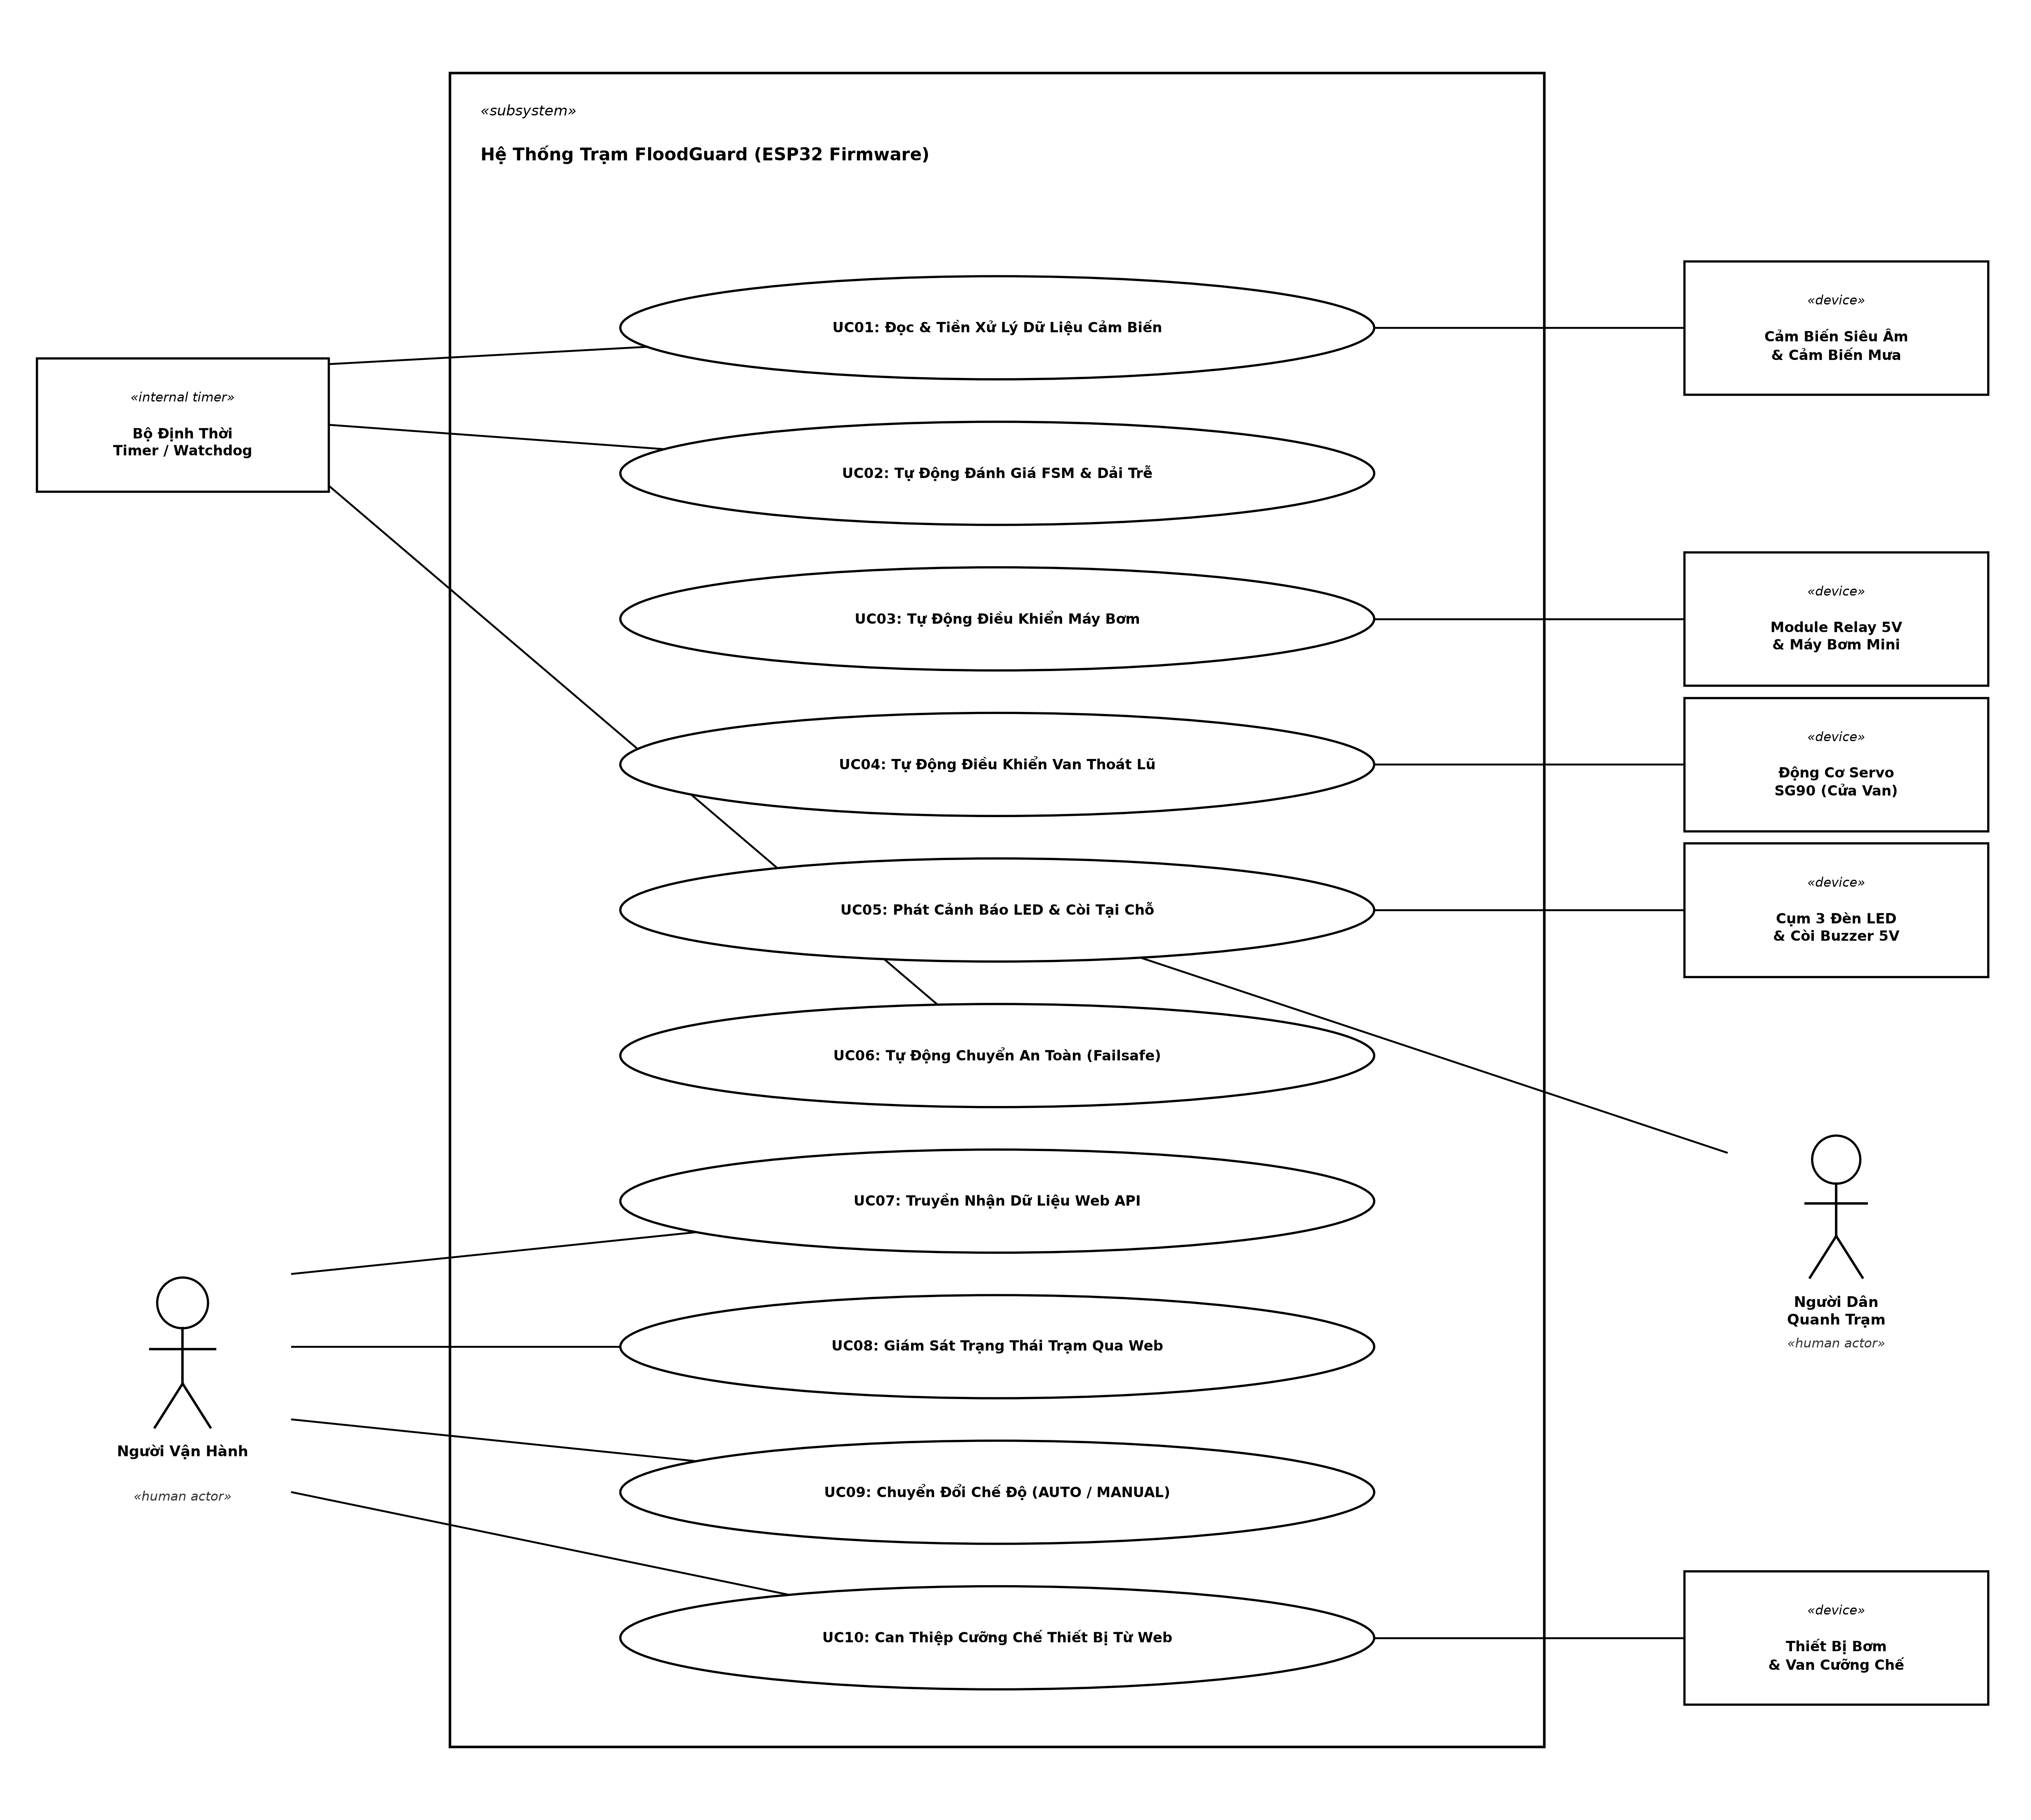
\includegraphics[width=0.92\textwidth]{figures/uc_overall_diagram.png}
    \caption{Sơ đồ Use Case tổng thể hệ thống FloodGuard chuẩn UML}
    \label{fig:uc_overall}
\end{figure}

\subsection{Đặc Tả Chi Tiết 10 Trường Hợp Sử Dụng (Use Cases)}

% --- UC01 ---
\subsubsection{UC01: Đọc và Tiền Xử Lý Dữ Liệu Cảm Biến}
\begin{itemize}
    \item \textbf{Mã định danh:} \texttt{UC01}
    \item \textbf{Tác nhân:}
    \begin{itemize}
        \item \textit{Môi trường:} Mặt thoáng nước dập dềnh (phản xạ siêu âm); Hạt mưa rơi / ngập nước (dẫn điện).
        \item \textit{Ngoại vi:} Cảm biến HC-SR04 (Trig/Echo), Cảm biến mưa FC-37 (DO/AO).
        \item \textit{Vi điều khiển:} ESP32 (GPIO Hardware Timers, ADC 12-bit).
    \end{itemize}
    \item \textbf{Mục tiêu:} Thu thập dữ liệu cảm biến sạch, triệt tiêu xung gai nhiễu điện từ (EMI) do máy bơm gây ra và quy đổi ra \% mực nước cùng các cấp độ mưa.
    \item \textbf{Tiền điều kiện:} Cảm biến được cấp nguồn ổn định; chân Trig/Echo và AO/DO nối đúng chân GPIO.
    \item \textbf{Luồng sự kiện chính:}
    \begin{enumerate}
        \item ESP32 kích xung phát 10$\mu$s chân Trig (GPIO 13), đọc độ rộng xung Echo (GPIO 12) bằng hàm \texttt{pulseIn()} với timeout 25ms.
        \item Áp dụng \textbf{Bộ lọc trung vị (Median Filter of 3 samples)}: Lấy 3 mẫu liên tiếp cách nhau 12ms, loại bỏ mẫu ngoài dải ($2\text{ cm} - 300\text{ cm}$), sắp xếp lấy mẫu ở giữa; nếu lỗi do sụt áp thì giữ giá trị hợp lệ gần nhất (\texttt{lastValidDistance}).
        \item Quy đổi khoảng cách sang phần trăm mực nước: $0\%$ (cạn $50\text{ cm}$) đến $100\%$ (đầy tràn $5\text{ cm}$).
        \item Đọc tín hiệu số \texttt{DO} (GPIO 34) và chân tương tự \texttt{AO} (GPIO 35, ADC 12-bit), phân loại 3 cấp độ: Mưa nhỏ ($< 2800$), Mưa to ($< 1800$), Ngập nước ($< 1100$).
    \end{enumerate}
    \item \textbf{Hậu điều kiện:} Cung cấp các thông số chuẩn hóa \texttt{waterPercent}, \texttt{currentDistance}, \texttt{rainRawADC}, \texttt{isRaining}, \texttt{isHeavyRain}, \texttt{isSubmerged} cho thuật toán FSM và Web Server.
\end{itemize}

\begin{figure}[H]
    \centering
    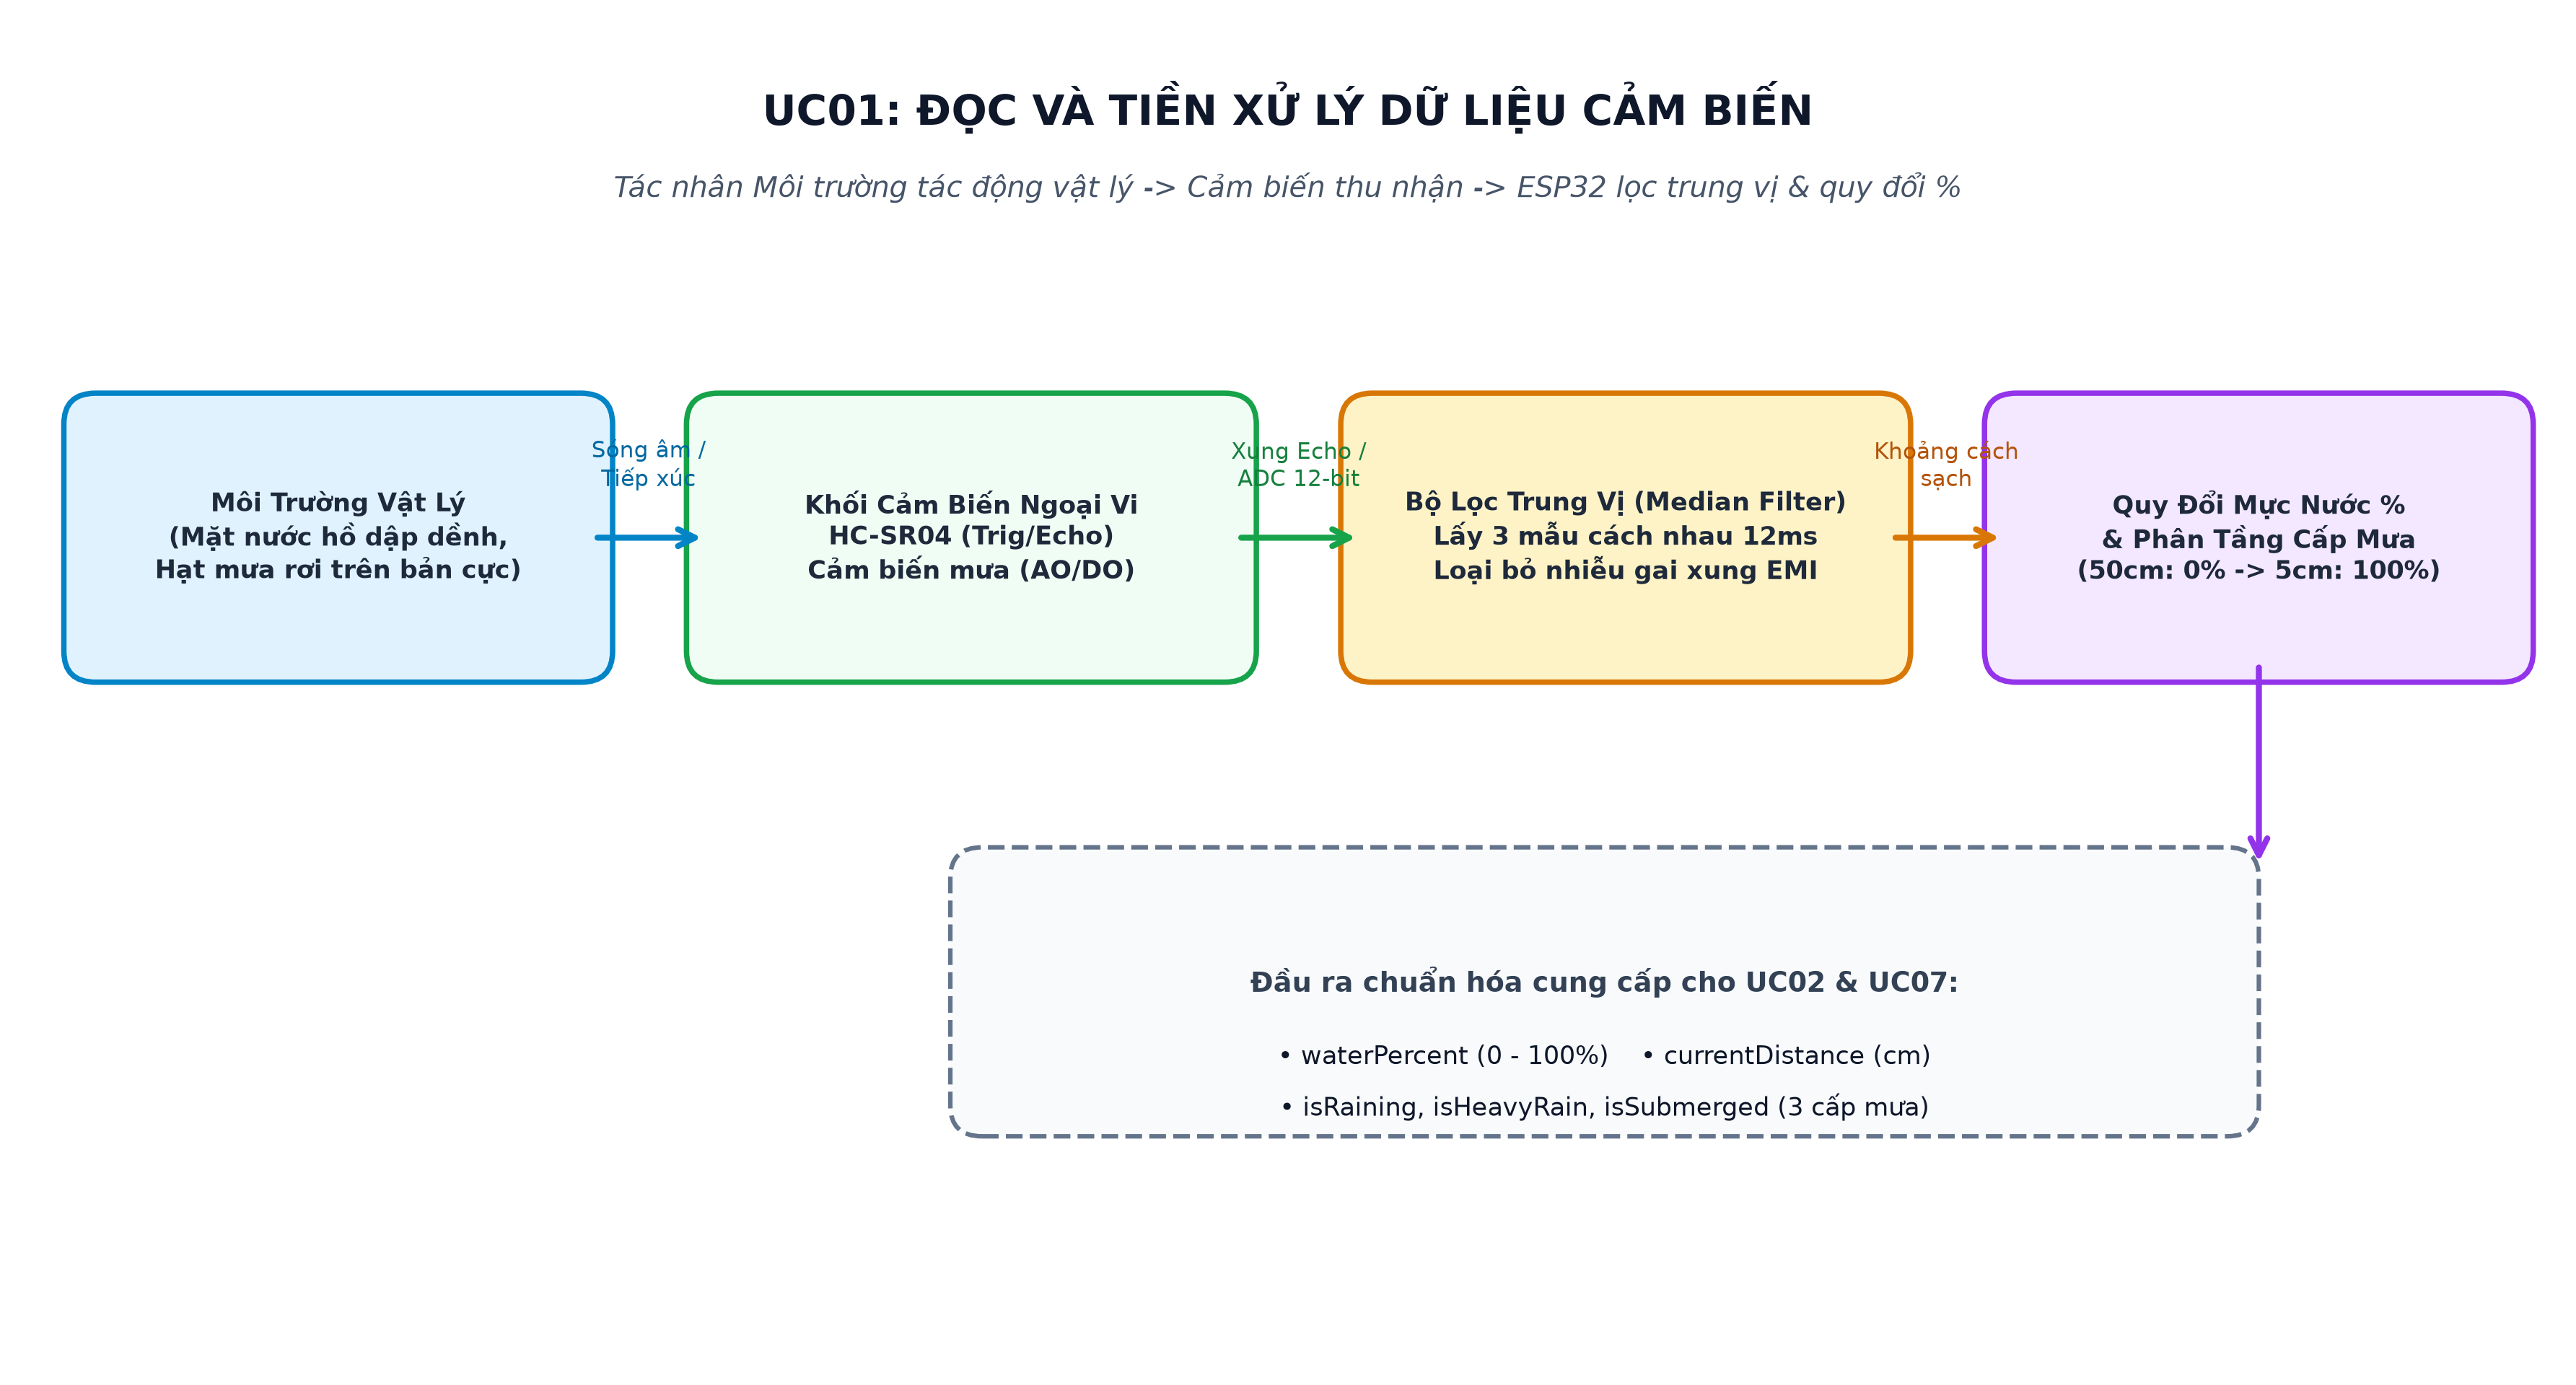
\includegraphics[width=0.88\textwidth]{figures/uc01_sensor_processing.png}
    \caption{Sơ đồ tương tác tác nhân UC01: Đọc và tiền xử lý dữ liệu cảm biến}
    \label{fig:uc01}
\end{figure}

% --- UC02 ---
\subsubsection{UC02: Tự Động Đánh Giá Ngưỡng Trạng Thái \& Xử Lý Chống Rung (Hysteresis)}
\begin{itemize}
    \item \textbf{Mã định danh:} \texttt{UC02}
    \item \textbf{Tác nhân:} ESP32 Firmware (Máy trạng thái hữu hạn -- Finite State Machine).
    \item \textbf{Mục tiêu:} Xác định trạng thái vận hành của trạm và triệt tiêu hiện tượng rung giật đóng/ngắt thiết bị liên tục (chattering/jittering) khi mặt nước dao động quanh biên ngưỡng.
    \item \textbf{Tiền điều kiện:} Hệ thống ở chế độ \texttt{AUTO MODE} và dữ liệu cảm biến từ \texttt{UC01} đã sẵn sàng.
    \item \textbf{Luồng sự kiện chính:}
    \begin{enumerate}
        \item ESP32 đối chiếu \texttt{waterPercent} và cấp độ mưa với bảng quy tắc 4 trạng thái:
        \begin{itemize}
            \item \textbf{NORMAL (An toàn):} Nước $\le 20\%$, tạnh mưa.
            \item \textbf{WARNING (Cảnh báo sớm):} Nước $21\% - 40\%$ hoặc phát hiện có mưa nhỏ.
            \item \textbf{DANGER (Nguy cơ ngập):} Nước $41\% - 70\%$ hoặc có mưa to.
            \item \textbf{CRITICAL (Nguy cấp):} Nước $\ge 71\%$ hoặc cảm biến mưa ngập hoàn toàn trong nước.
        \end{itemize}
        \item Áp dụng cơ chế \textbf{Dải trễ (Hysteresis)} khi nước rút:
        \begin{itemize}
            \item Từ CRITICAL hạ xuống DANGER khi nước $< 71\%$ và hết ngập cảm biến mưa.
            \item Từ DANGER hạ xuống WARNING khi nước rút sâu $< 40\%$ (chênh lệch biên $\Delta = 1\%$ chống rung giật) và không còn mưa to.
            \item Từ WARNING hạ về NORMAL chỉ khi nước rút sâu $< 20\%$ và tạnh mưa hoàn toàn.
        \end{itemize}
    \end{enumerate}
    \item \textbf{Hậu điều kiện:} Biến trạng thái \texttt{sysState} được cập nhật chính xác, kích hoạt điều khiển đồng bộ cho UC03, UC04 và UC05.
\end{itemize}

\begin{figure}[H]
    \centering
    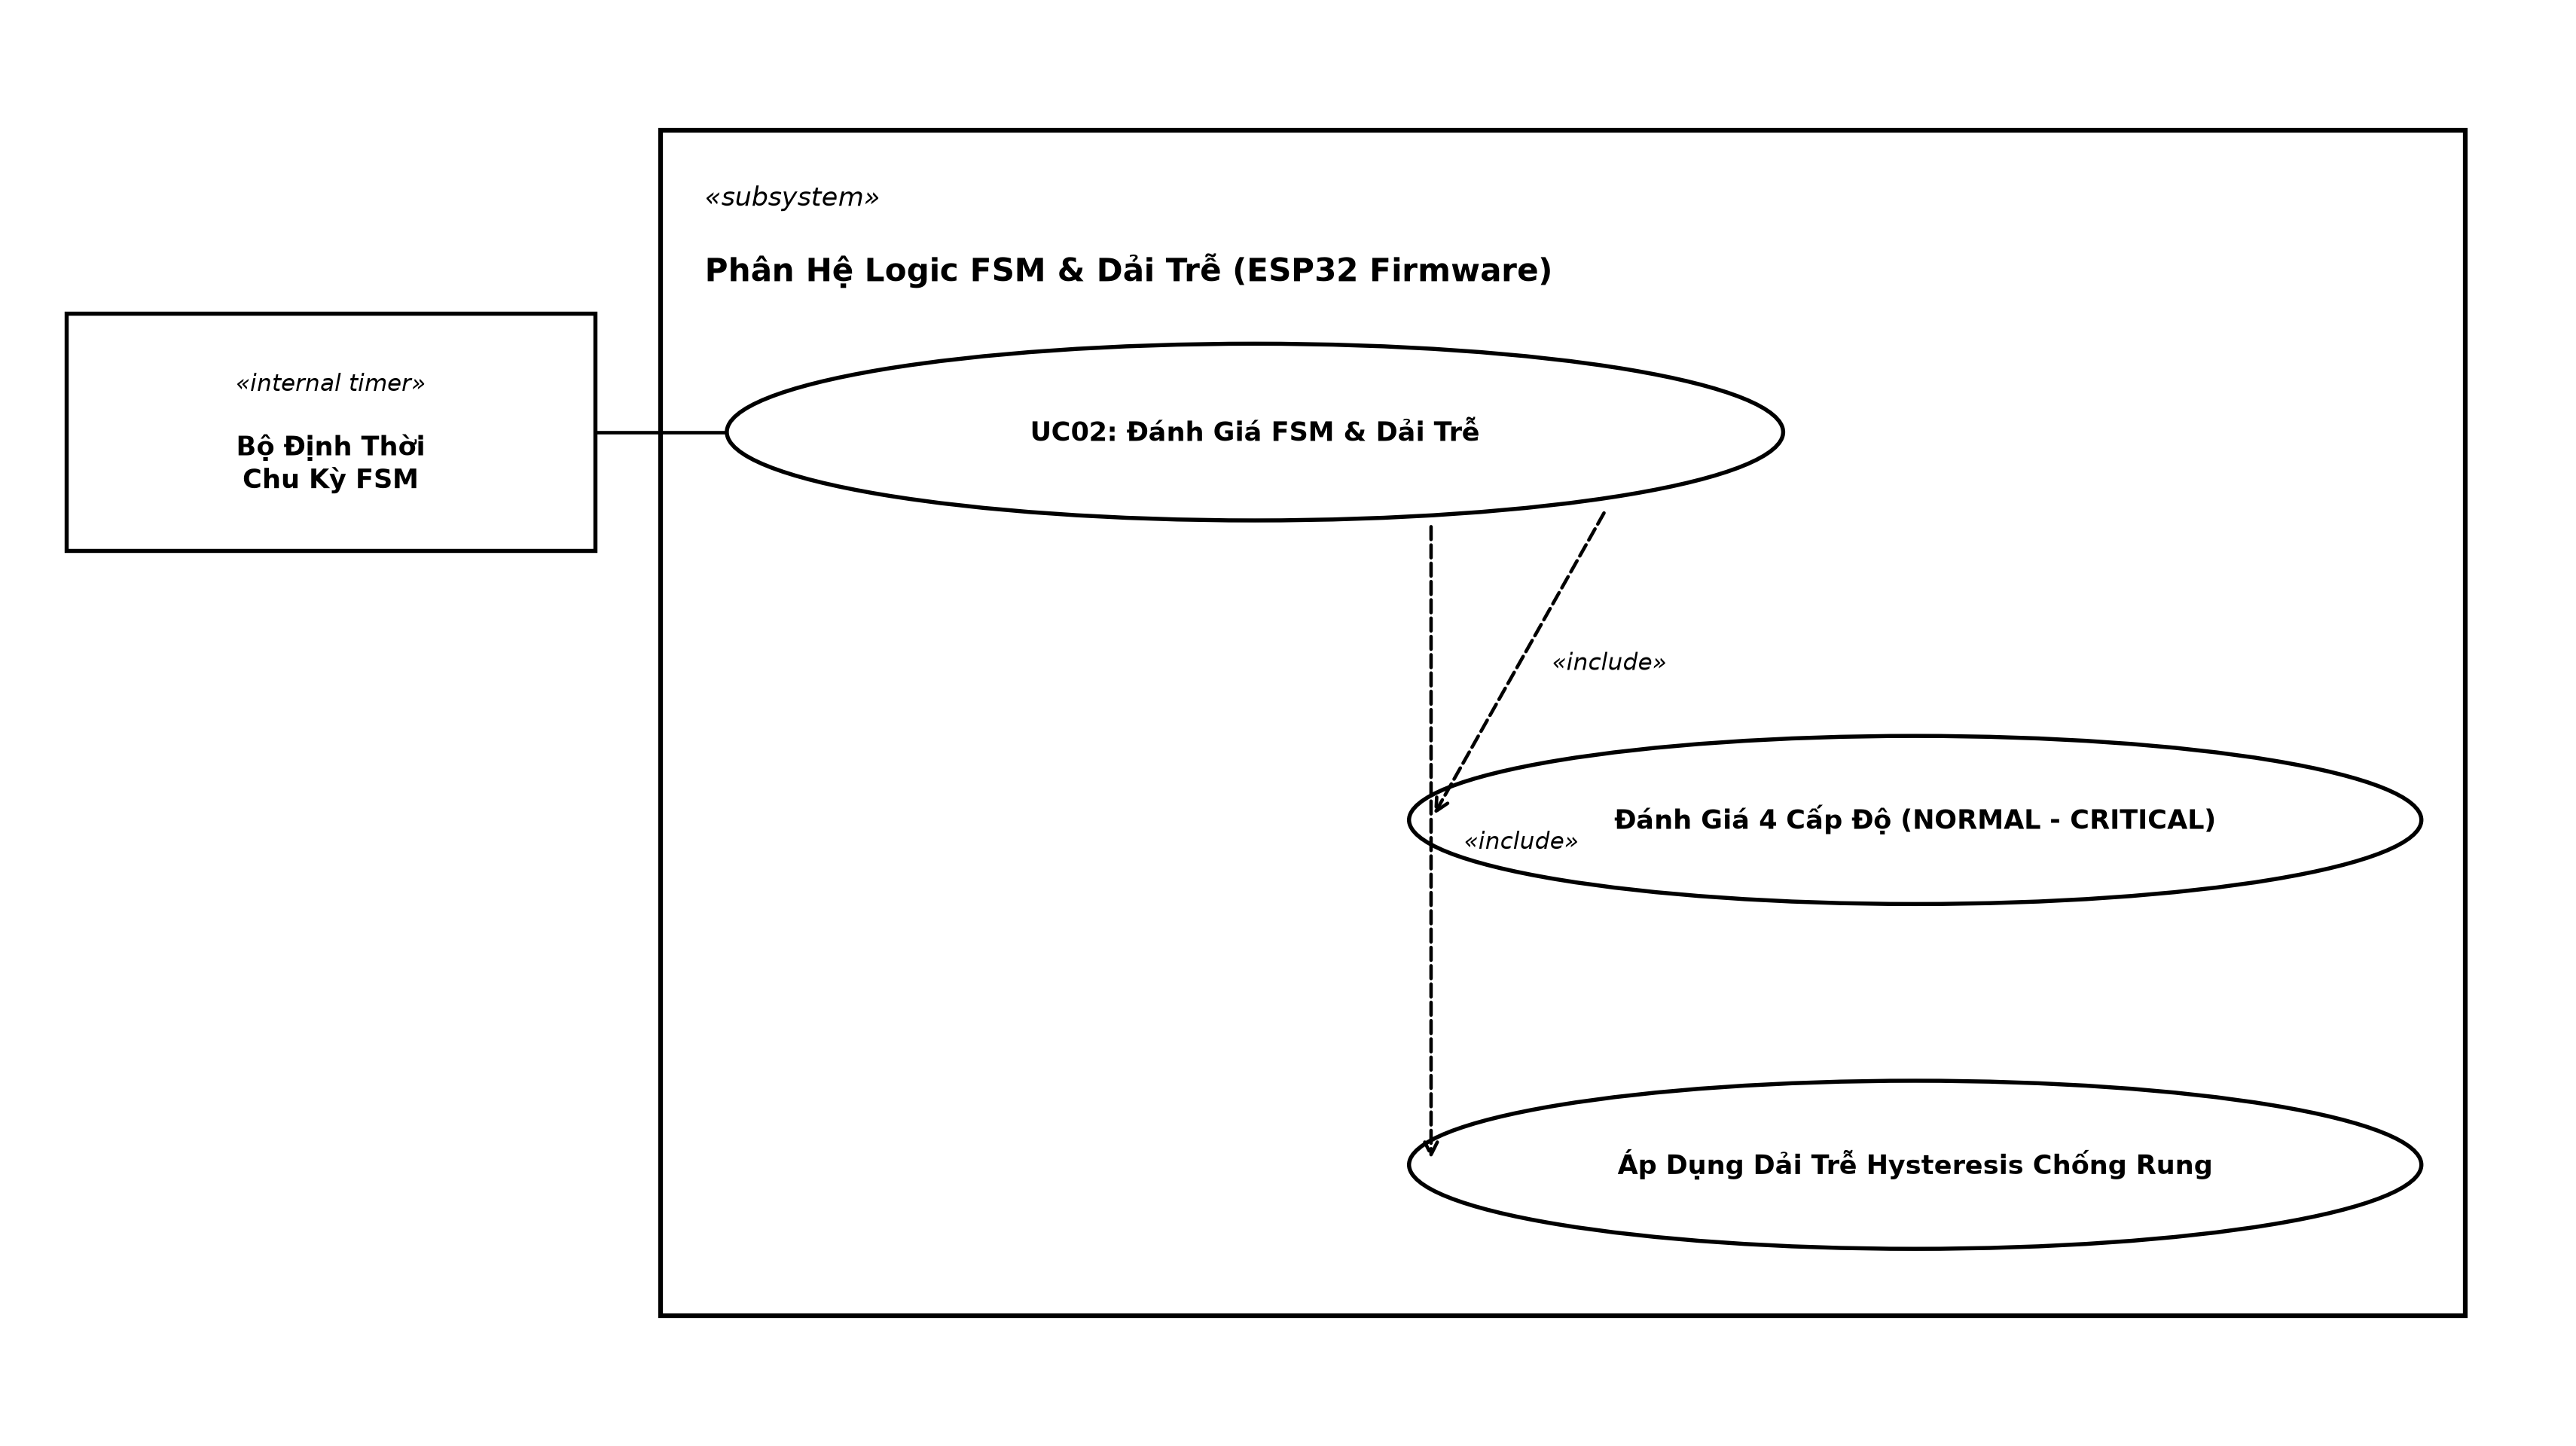
\includegraphics[width=0.88\textwidth]{figures/uc02_fsm_hysteresis.png}
    \caption{Sơ đồ tương tác tác nhân UC02: Tự động đánh giá FSM \& Hysteresis}
    \label{fig:uc02}
\end{figure}

% --- UC03 ---
\subsubsection{UC03: Tự Động Điều Khiển Máy Bơm Thoát Nước}
\begin{itemize}
    \item \textbf{Mã định danh:} \texttt{UC03}
    \item \textbf{Tác nhân:}
    \begin{itemize}
        \item \textit{Vi điều khiển:} ESP32 (GPIO 23).
        \item \textit{Ngoại vi:} Module Relay 1 kênh 5V (Active LOW, cách ly quang), Máy bơm mini 5V.
        \item \textit{Môi trường:} Khối nước cần được bơm tiêu thoát ra ngoài bể chứa.
    \end{itemize}
    \item \textbf{Mục tiêu:} Tự động kích hoạt máy bơm khi đạt ngưỡng nguy cơ và ngừng bơm dứt điểm khi nước đã rút về mức an toàn.
    \item \textbf{Tiền điều kiện:} Hệ thống ở chế độ \texttt{isAutoMode == true}.
    \item \textbf{Luồng sự kiện chính:}
    \begin{enumerate}
        \item Khi FSM chạm mức \texttt{DANGER} (nước $\ge 41\%$ hoặc mưa to) hoặc \texttt{CRITICAL}: ESP32 bật bơm bằng cấu hình \texttt{pinMode(PIN\_RELAY, OUTPUT)} và kéo xuống mức \texttt{LOW}. Tiếp điểm Relay đóng, cấp nguồn cho máy bơm chạy.
        \item Khi nước rút xuống dưới ngưỡng an toàn $< 40\%$ và tạnh mưa to: ESP32 tắt bơm bằng \textbf{kỹ thuật High-Z} \texttt{pinMode(PIN\_RELAY, INPUT)}. Chân GPIO thả nổi trở kháng cao, triệt tiêu hoàn toàn dòng rò $1.5\text{ mA}$ qua optocoupler 5V, đảm bảo bơm ngắt hoàn toàn $100\%$.
    \end{enumerate}
    \item \textbf{Hậu điều kiện:} Bơm duy trì hoạt động hoặc ngắt nghỉ đúng quy trình an toàn, bảo vệ relay và máy bơm.
\end{itemize}

\begin{figure}[H]
    \centering
    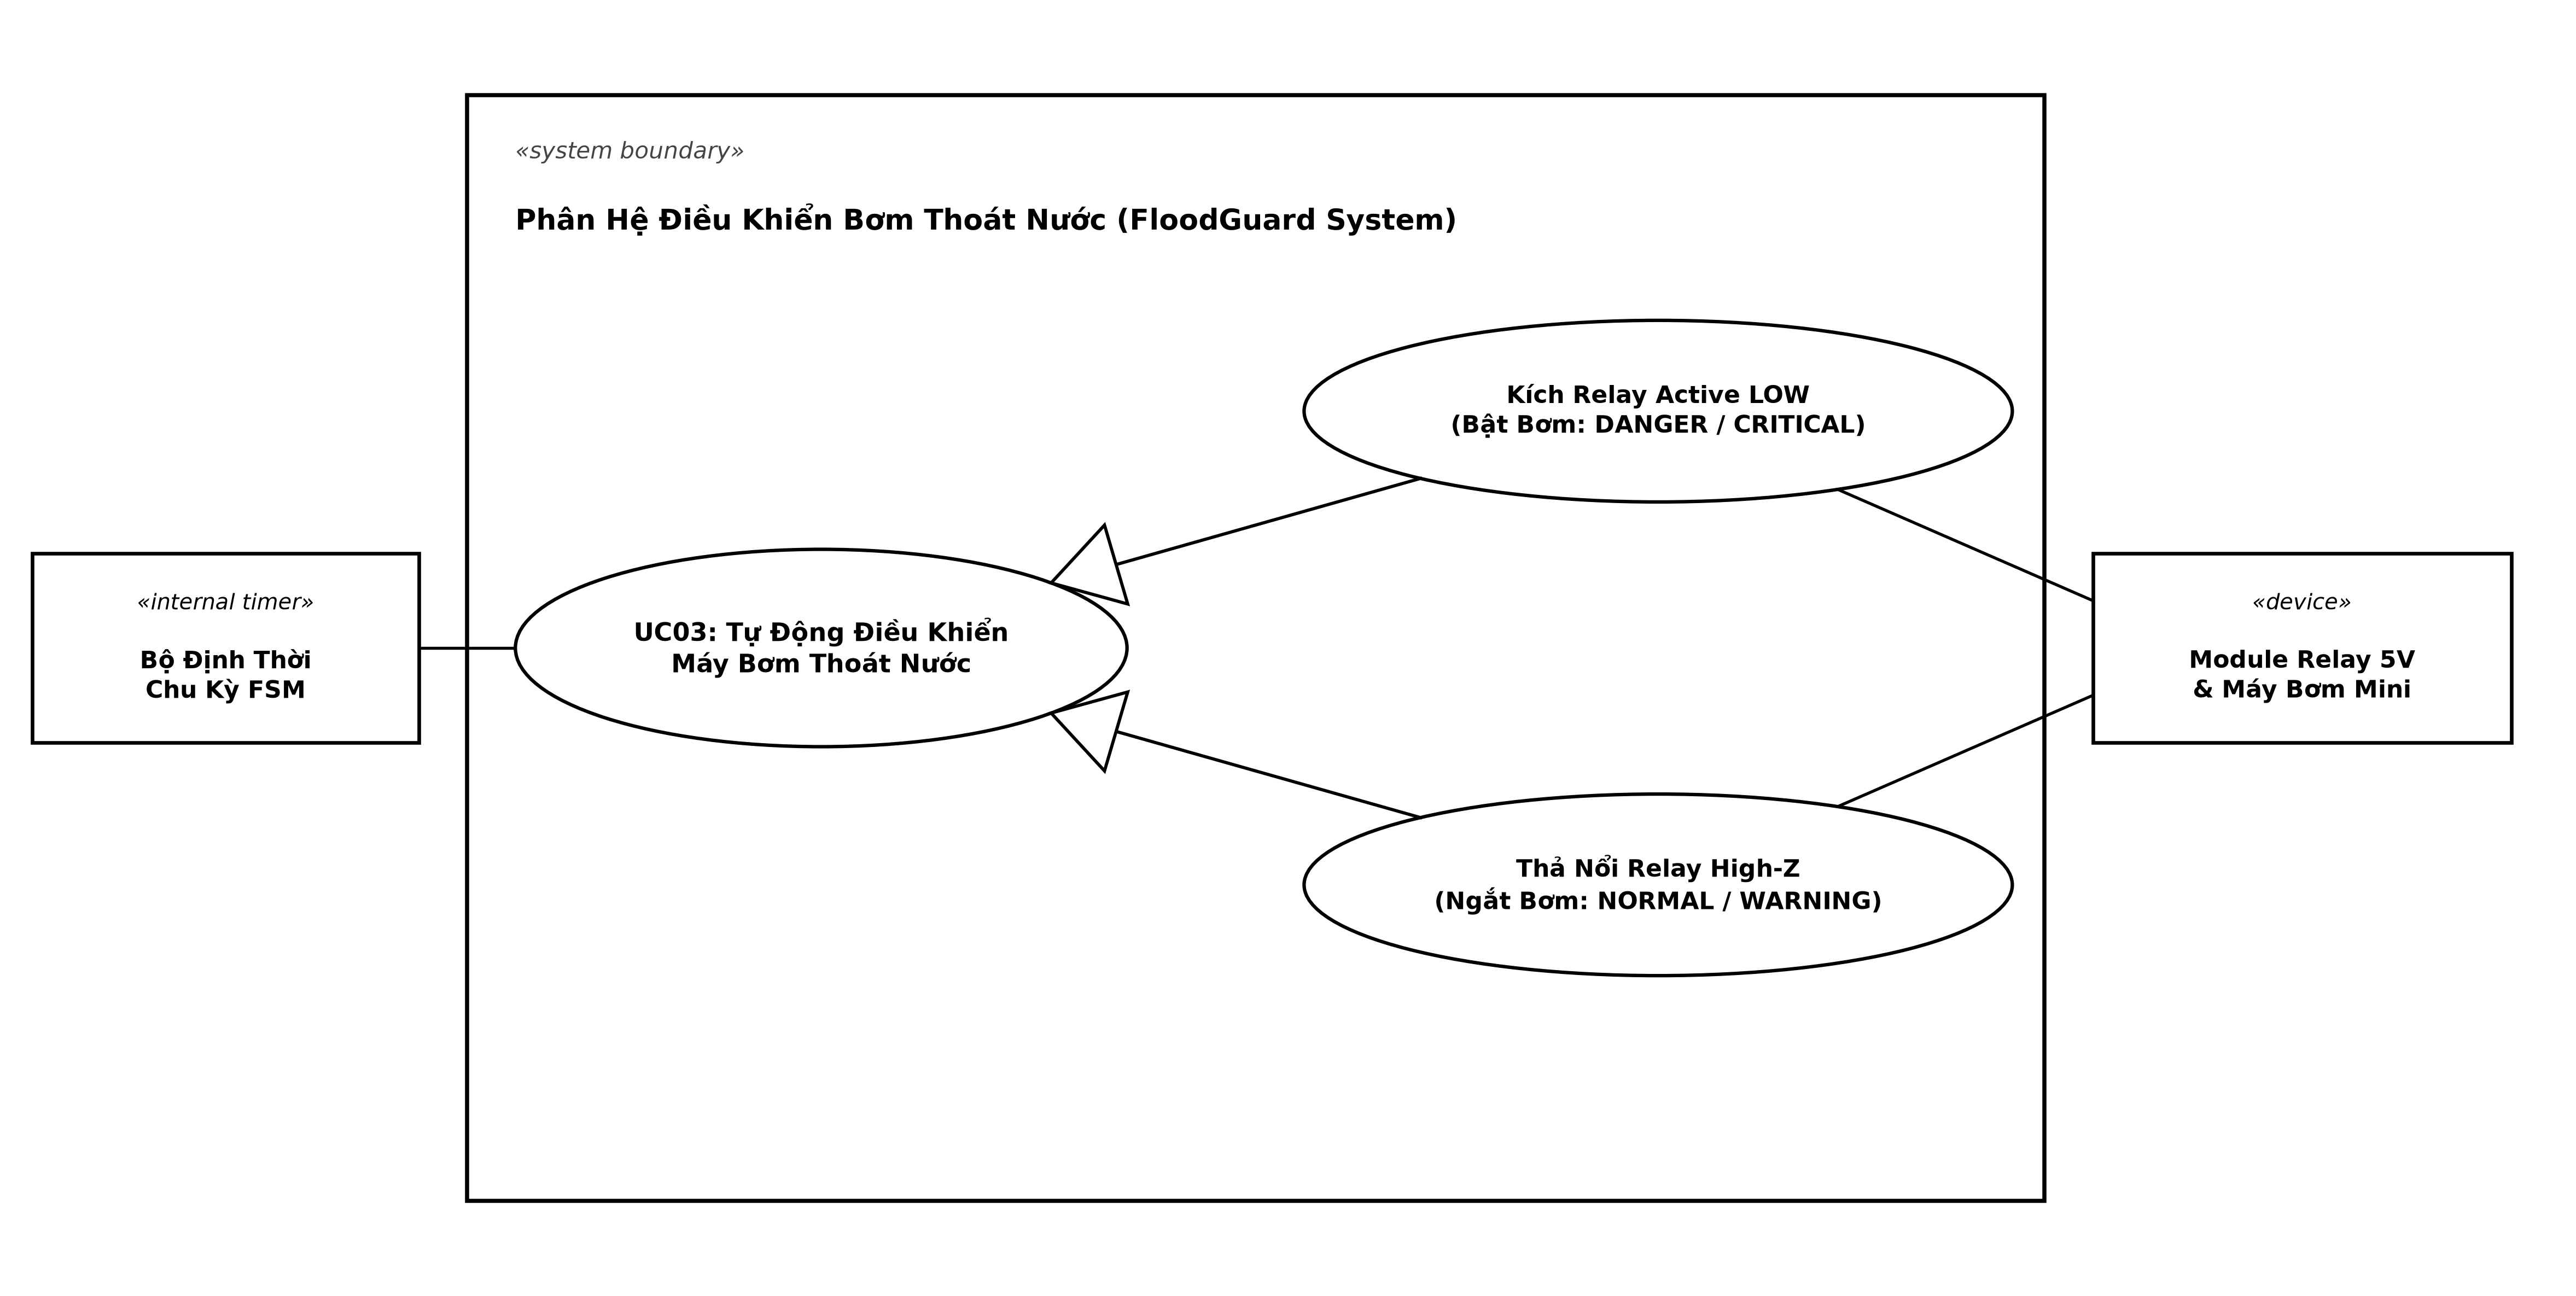
\includegraphics[width=0.88\textwidth]{figures/uc03_pump_control.png}
    \caption{Sơ đồ tương tác tác nhân UC03: Tự động điều khiển máy bơm thoát nước}
    \label{fig:uc03}
\end{figure}

% --- UC04 ---
\subsubsection{UC04: Tự Động Điều Khiển Góc Mở Van Thoát Lũ}
\begin{itemize}
    \item \textbf{Mã định danh:} \texttt{UC04}
    \item \textbf{Tác nhân:}
    \begin{itemize}
        \item \textit{Vi điều khiển:} ESP32 (GPIO 27 -- PWM Timer Hardware).
        \item \textit{Ngoại vi:} Động cơ Servo SG90, Cửa van xả lũ hồ thu.
        \item \textit{Môi trường:} Lưu lượng dòng chảy nước lũ xả qua cửa cống.
    \end{itemize}
    \item \textbf{Mục tiêu:} Tự động điều tiết lưu lượng xả lũ tương ứng theo mức độ ngập của trạm.
    \item \textbf{Tiền điều kiện:} Hệ thống ở chế độ \texttt{isAutoMode == true}.
    \item \textbf{Luồng sự kiện chính:}
    \begin{enumerate}
        \item ESP32 ánh xạ trạng thái FSM sang góc mở van:
        \begin{itemize}
            \item \texttt{NORMAL} hoặc \texttt{WARNING}: Góc mở $0^\circ$ (Độ mở $0\%$ -- Đóng kín van giữ nước).
            \item \texttt{DANGER}: Góc mở $90^\circ$ (Độ mở $50\%$ -- Mở xả dòng chảy mức trung bình).
            \item \texttt{CRITICAL}: Góc mở $180^\circ$ (Độ mở $100\%$ -- Mở xả lũ tối đa khẩn cấp).
        \end{itemize}
        \item Xuất xung PWM độ rộng $500\mu\text{s} - 2400\mu\text{s}$ đến chân tín hiệu động cơ Servo SG90 để kéo trục van mở đúng góc.
    \end{enumerate}
    \item \textbf{Hậu điều kiện:} Cửa van đạt góc mở chính xác, duy trì ổn định dòng xả lũ tương ứng.
\end{itemize}

\begin{figure}[H]
    \centering
    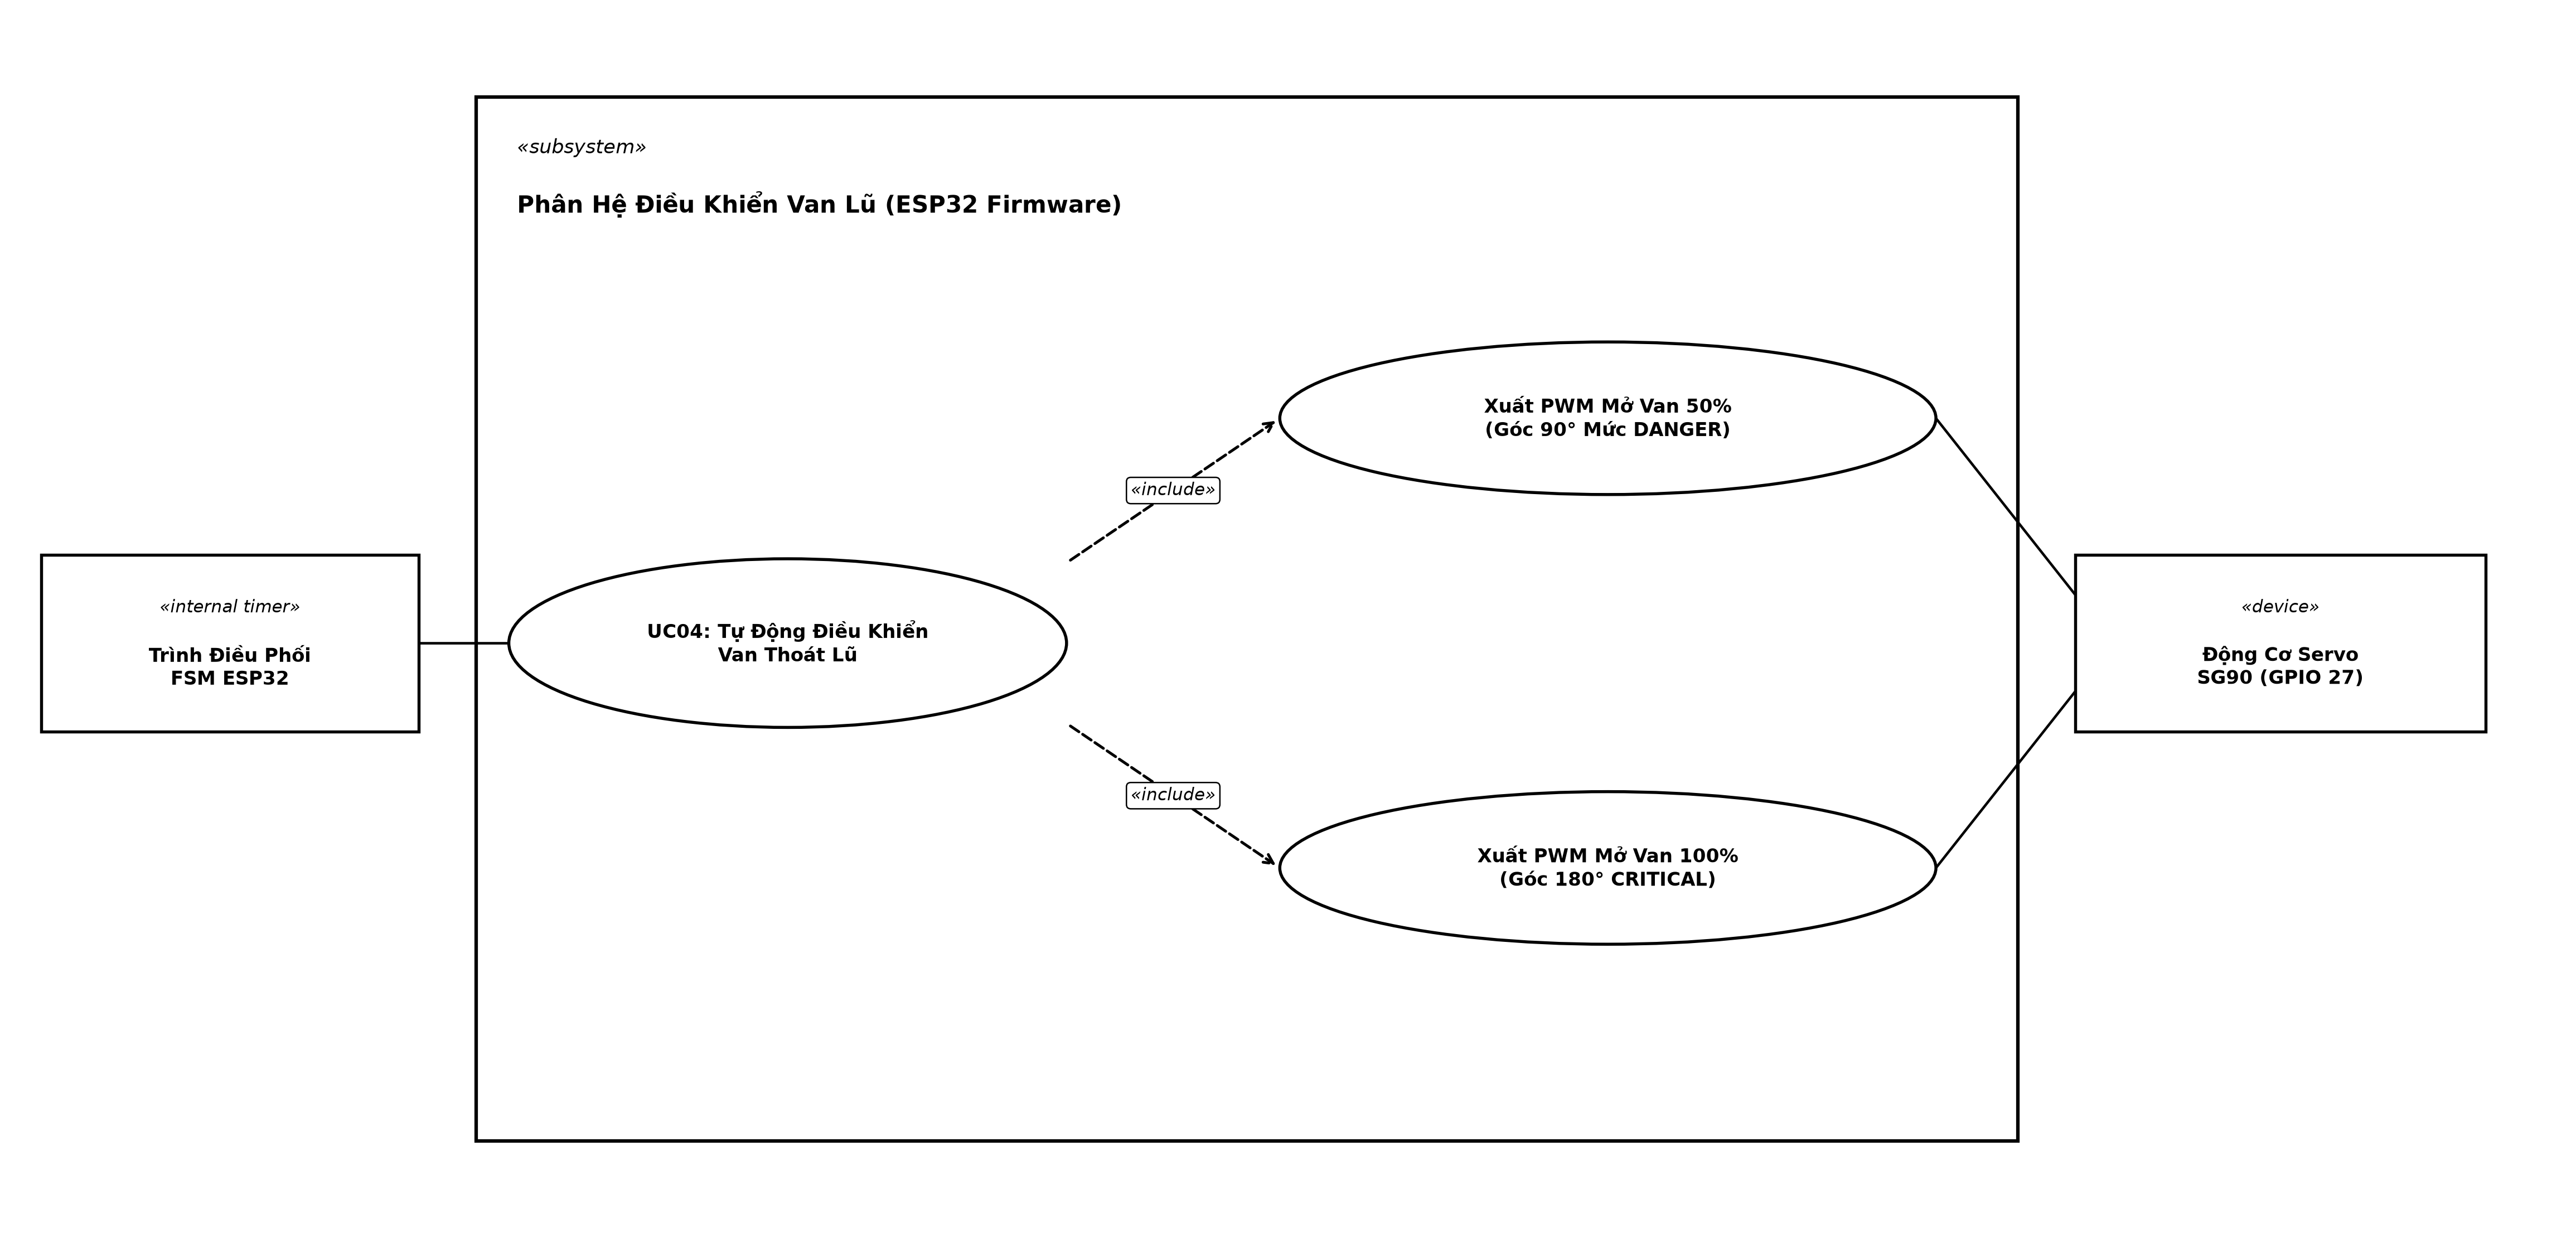
\includegraphics[width=0.88\textwidth]{figures/uc04_valve_control.png}
    \caption{Sơ đồ tương tác tác nhân UC04: Tự động điều khiển góc mở van thoát lũ}
    \label{fig:uc04}
\end{figure}

% --- UC05 ---
\subsubsection{UC05: Tự Động Phát Tín Hiệu Cảnh Báo Tại Trạm (LED \& Buzzer)}
\begin{itemize}
    \item \textbf{Mã định danh:} \texttt{UC05}
    \item \textbf{Tác nhân:}
    \begin{itemize}
        \item \textit{Vi điều khiển:} ESP32 (GPIO 21, 19, 18, 4).
        \item \textit{Ngoại vi:} Cụm 3 LED chỉ thị (Xanh D21, Vàng D19, Đỏ D18), Còi báo động Active Buzzer 5V (D4).
        \item \textit{Con người:} Người dân và kỹ thuật viên xung quanh trạm đo (tiếp nhận âm thanh/ánh sáng).
    \end{itemize}
    \item \textbf{Mục tiêu:} Cảnh báo trực quan tại chỗ bằng đèn LED và âm thanh đa cấp độ mà không gây chặn luồng xử lý (\textit{Non-blocking}).
    \item \textbf{Tiền điều kiện:} Chân GPIO LED và Buzzer được khởi tạo OUTPUT.
    \item \textbf{Luồng sự kiện chính:}
    \begin{enumerate}
        \item Quản lý nhịp bíp bằng biến thời gian \texttt{millis()}, không sử dụng hàm \texttt{delay()}:
        \begin{itemize}
            \item \textbf{NORMAL:} LED Xanh bật sáng; LED Vàng và Đỏ tắt; Còi tắt hoàn toàn (\texttt{noTone}).
            \item \textbf{WARNING:} LED Vàng bật sáng; Còi phát xung $1000\text{ Hz}$ nhịp thưa (bíp 120ms mỗi chu kỳ 1.5 giây).
            \item \textbf{DANGER:} LED Đỏ bật sáng; Còi phát xung $1800\text{ Hz}$ nhịp dồn dập (kêu 150ms, ngắt 150ms theo chu kỳ 300ms).
            \item \textbf{CRITICAL:} LED Đỏ chớp nhấp nháy liên tục chu kỳ 100ms; Còi hú liên tục không ngắt ở tần số cao $2500\text{ Hz}$.
        \end{itemize}
    \end{enumerate}
    \item \textbf{Hậu điều kiện:} Trạm phát tín hiệu báo động chuẩn xác, âm thanh tương thích với cấp độ nguy hiểm.
\end{itemize}

\begin{figure}[H]
    \centering
    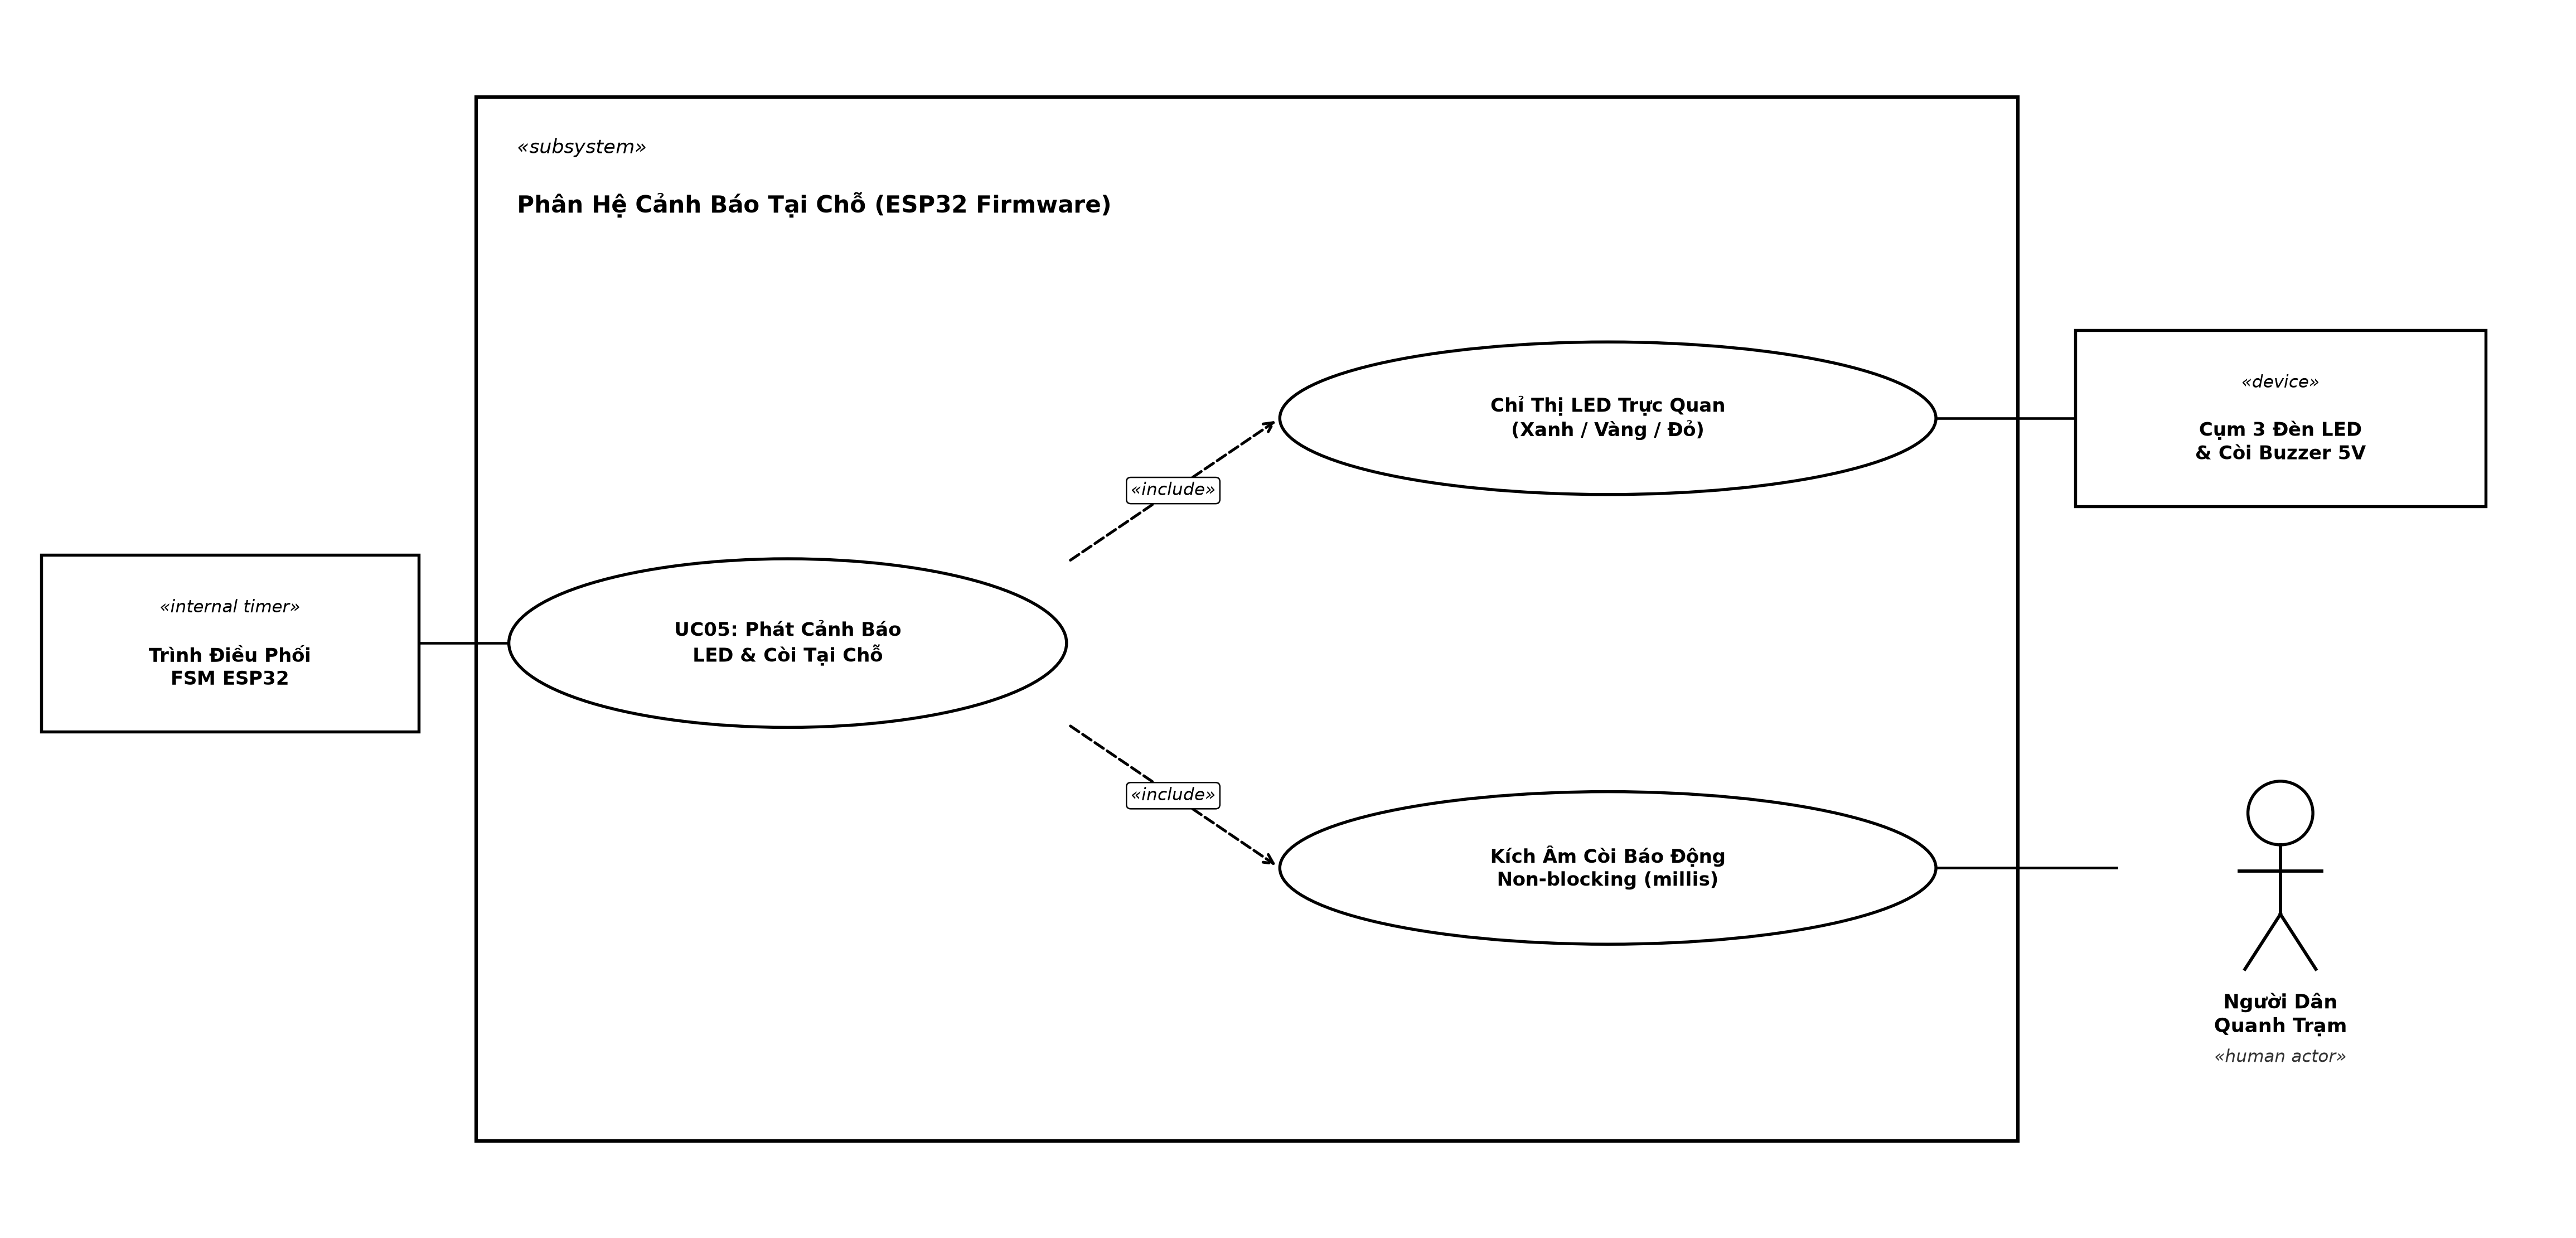
\includegraphics[width=0.88\textwidth]{figures/uc05_signaling_buzzer_led.png}
    \caption{Sơ đồ tương tác tác nhân UC05: Tự động phát tín hiệu cảnh báo tại trạm}
    \label{fig:uc05}
\end{figure}

% --- UC06 ---
\subsubsection{UC06: Tự Động Chuyển Đổi An Toàn Khi Mất Kết Nối Mạng (Failsafe to AUTO)}
\begin{itemize}
    \item \textbf{Mã định danh:} \texttt{UC06}
    \item \textbf{Tác nhân:}
    \begin{itemize}
        \item \textit{Hệ thống:} Bộ định thời giám sát Heartbeat / Failsafe của ESP32.
        \item \textit{Mạng truyền thông:} Kết nối sóng Wi-Fi Client.
    \end{itemize}
    \item \textbf{Mục tiêu:} Bảo vệ trạm tự động chống tràn bể khi người vận hành mất quyền giám sát từ xa hoặc rớt mạng Wi-Fi.
    \item \textbf{Tiền điều kiện:} Hệ thống đang ở chế độ thủ công \texttt{MANUAL MODE}.
    \item \textbf{Luồng sự kiện chính:}
    \begin{enumerate}
        \item ESP32 liên tục theo dõi thời điểm nhận bản tin HTTP request cuối cùng từ Client.
        \item Nếu phát hiện mất kết nối Wi-Fi hoặc mất heartbeat từ trình duyệt vượt quá thời gian quy định (Timeout):
        \begin{itemize}
            \item ESP32 lập tức phát tín hiệu cảnh báo mất kết nối mạng.
            \item Cưỡng chế đảo cờ \texttt{isAutoMode = true} (chuyển ngay về \texttt{AUTO MODE}).
            \item Trao lại quyền điều khiển van xả và máy bơm cho thuật toán FSM và dữ liệu cảm biến.
        \end{itemize}
    \end{enumerate}
    \item \textbf{Hậu điều kiện:} Trạm duy trì tính năng điều khiển tự trị (\textit{Autonomous Controller}), ngăn ngừa nguy cơ ngập úng khi người dùng bỏ quên chế độ thủ công.
\end{itemize}

\begin{figure}[H]
    \centering
    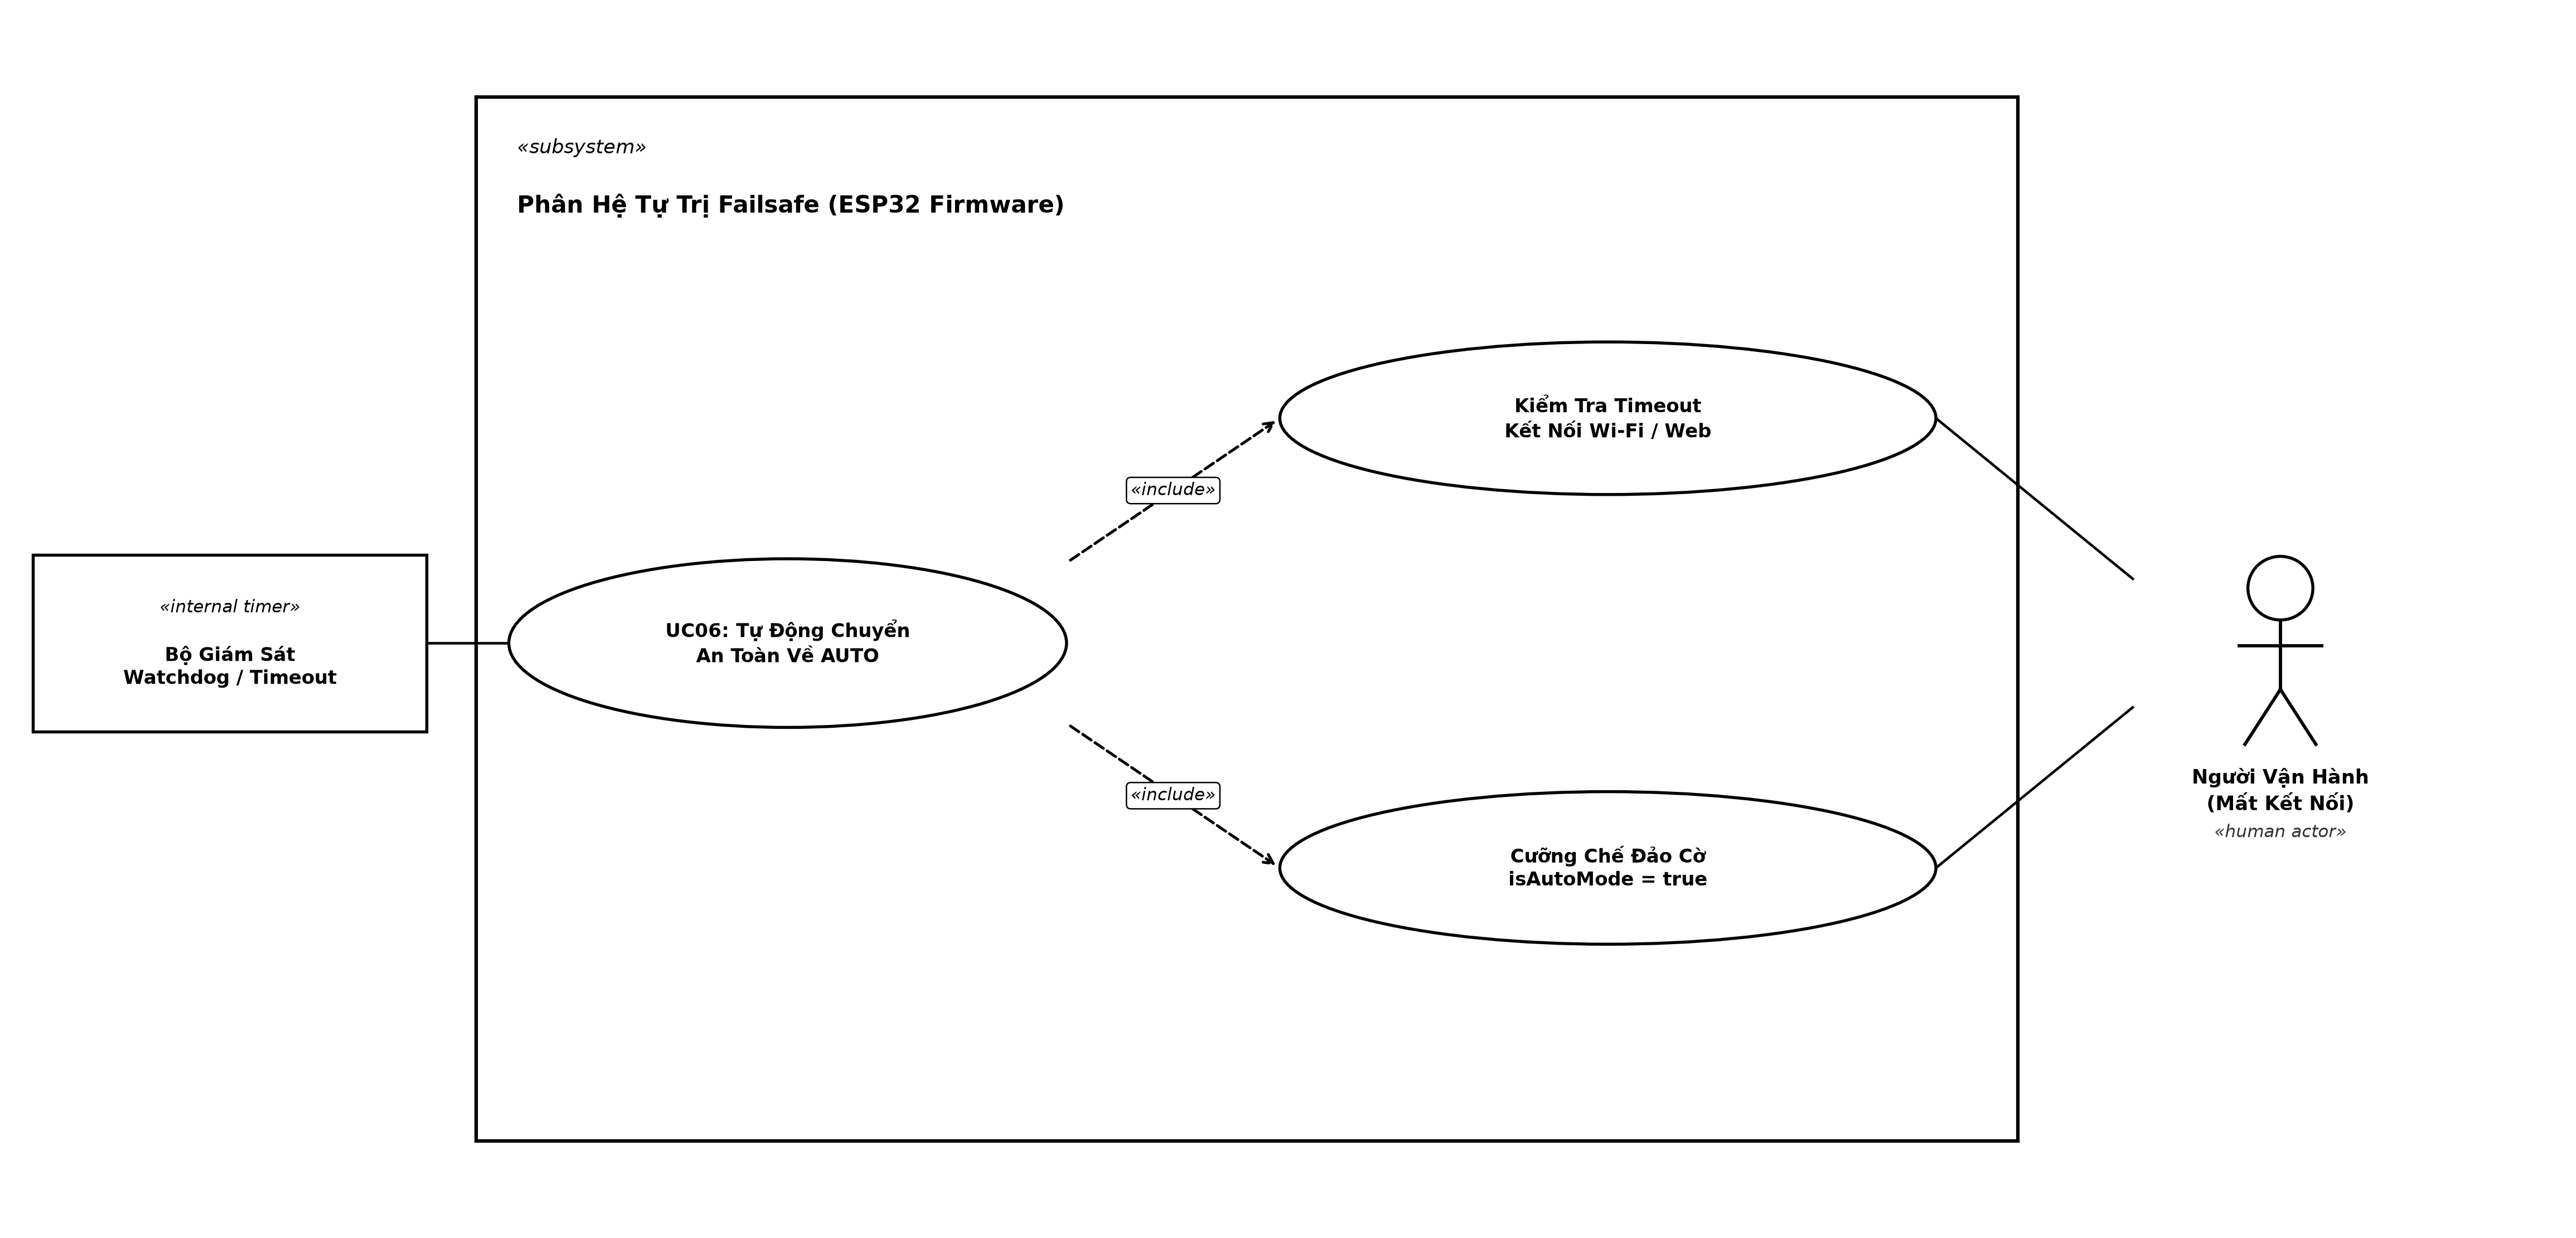
\includegraphics[width=0.88\textwidth]{figures/uc06_network_failsafe.png}
    \caption{Sơ đồ tương tác tác nhân UC06: Tự động chuyển đổi an toàn khi mất mạng}
    \label{fig:uc06}
\end{figure}

% --- UC07 ---
\subsubsection{UC07: Truyền Nhận Dữ Liệu Thời Gian Thực Qua Giao Thức Web (Telemetry \& API)}
\begin{itemize}
    \item \textbf{Mã định danh:} \texttt{UC07}
    \item \textbf{Tác nhân:}
    \begin{itemize}
        \item \textit{Vi điều khiển:} ESP32 Web Server (thư viện \texttt{WebServer.h}, cổng 80).
        \item \textit{Mạng \& Phần mềm:} Trình duyệt Web máy tính / điện thoại qua mạng Wi-Fi (SoftAP hoặc Station).
    \end{itemize}
    \item \textbf{Mục tiêu:} Cung cấp các giao diện lập trình ứng dụng (REST API endpoints) đóng gói JSON để truyền tải thông số đo và nhận lệnh điều khiển.
    \item \textbf{Tiền điều kiện:} Web Server khởi động thành công (\texttt{server.begin()}) trên cổng 80; Client kết nối cùng dải mạng.
    \item \textbf{Luồng sự kiện chính:}
    \begin{enumerate}
        \item \texttt{GET /}: Trả về toàn bộ mã nguồn giao diện Web Dashboard (HTML/CSS/JS) lưu trong bộ nhớ Flash \texttt{PROGMEM}.
        \item \texttt{GET /api/status}: Đóng gói dữ liệu chuỗi JSON chuẩn:
        \begin{lstlisting}[language=C]
{"water":45, "distance":29.8, "rain":true, "rain_adc":1450, 
 "state":"DANGER", "mode":"AUTO", "pump":true, "valve":50, "buzzer":"FAST"}
        \end{lstlisting}
        \item \texttt{GET /api/control?action=...}: Tiếp nhận các tham số lệnh (\texttt{mode\_toggle}, \texttt{pump\_toggle}, \texttt{valve\_0}, \texttt{valve\_50}, \texttt{valve\_100}).
    \end{enumerate}
    \item \textbf{Hậu điều kiện:} Dữ liệu thời gian thực được đồng bộ hai chiều liên tục giữa ESP32 và Web Client.
\end{itemize}

\begin{figure}[H]
    \centering
    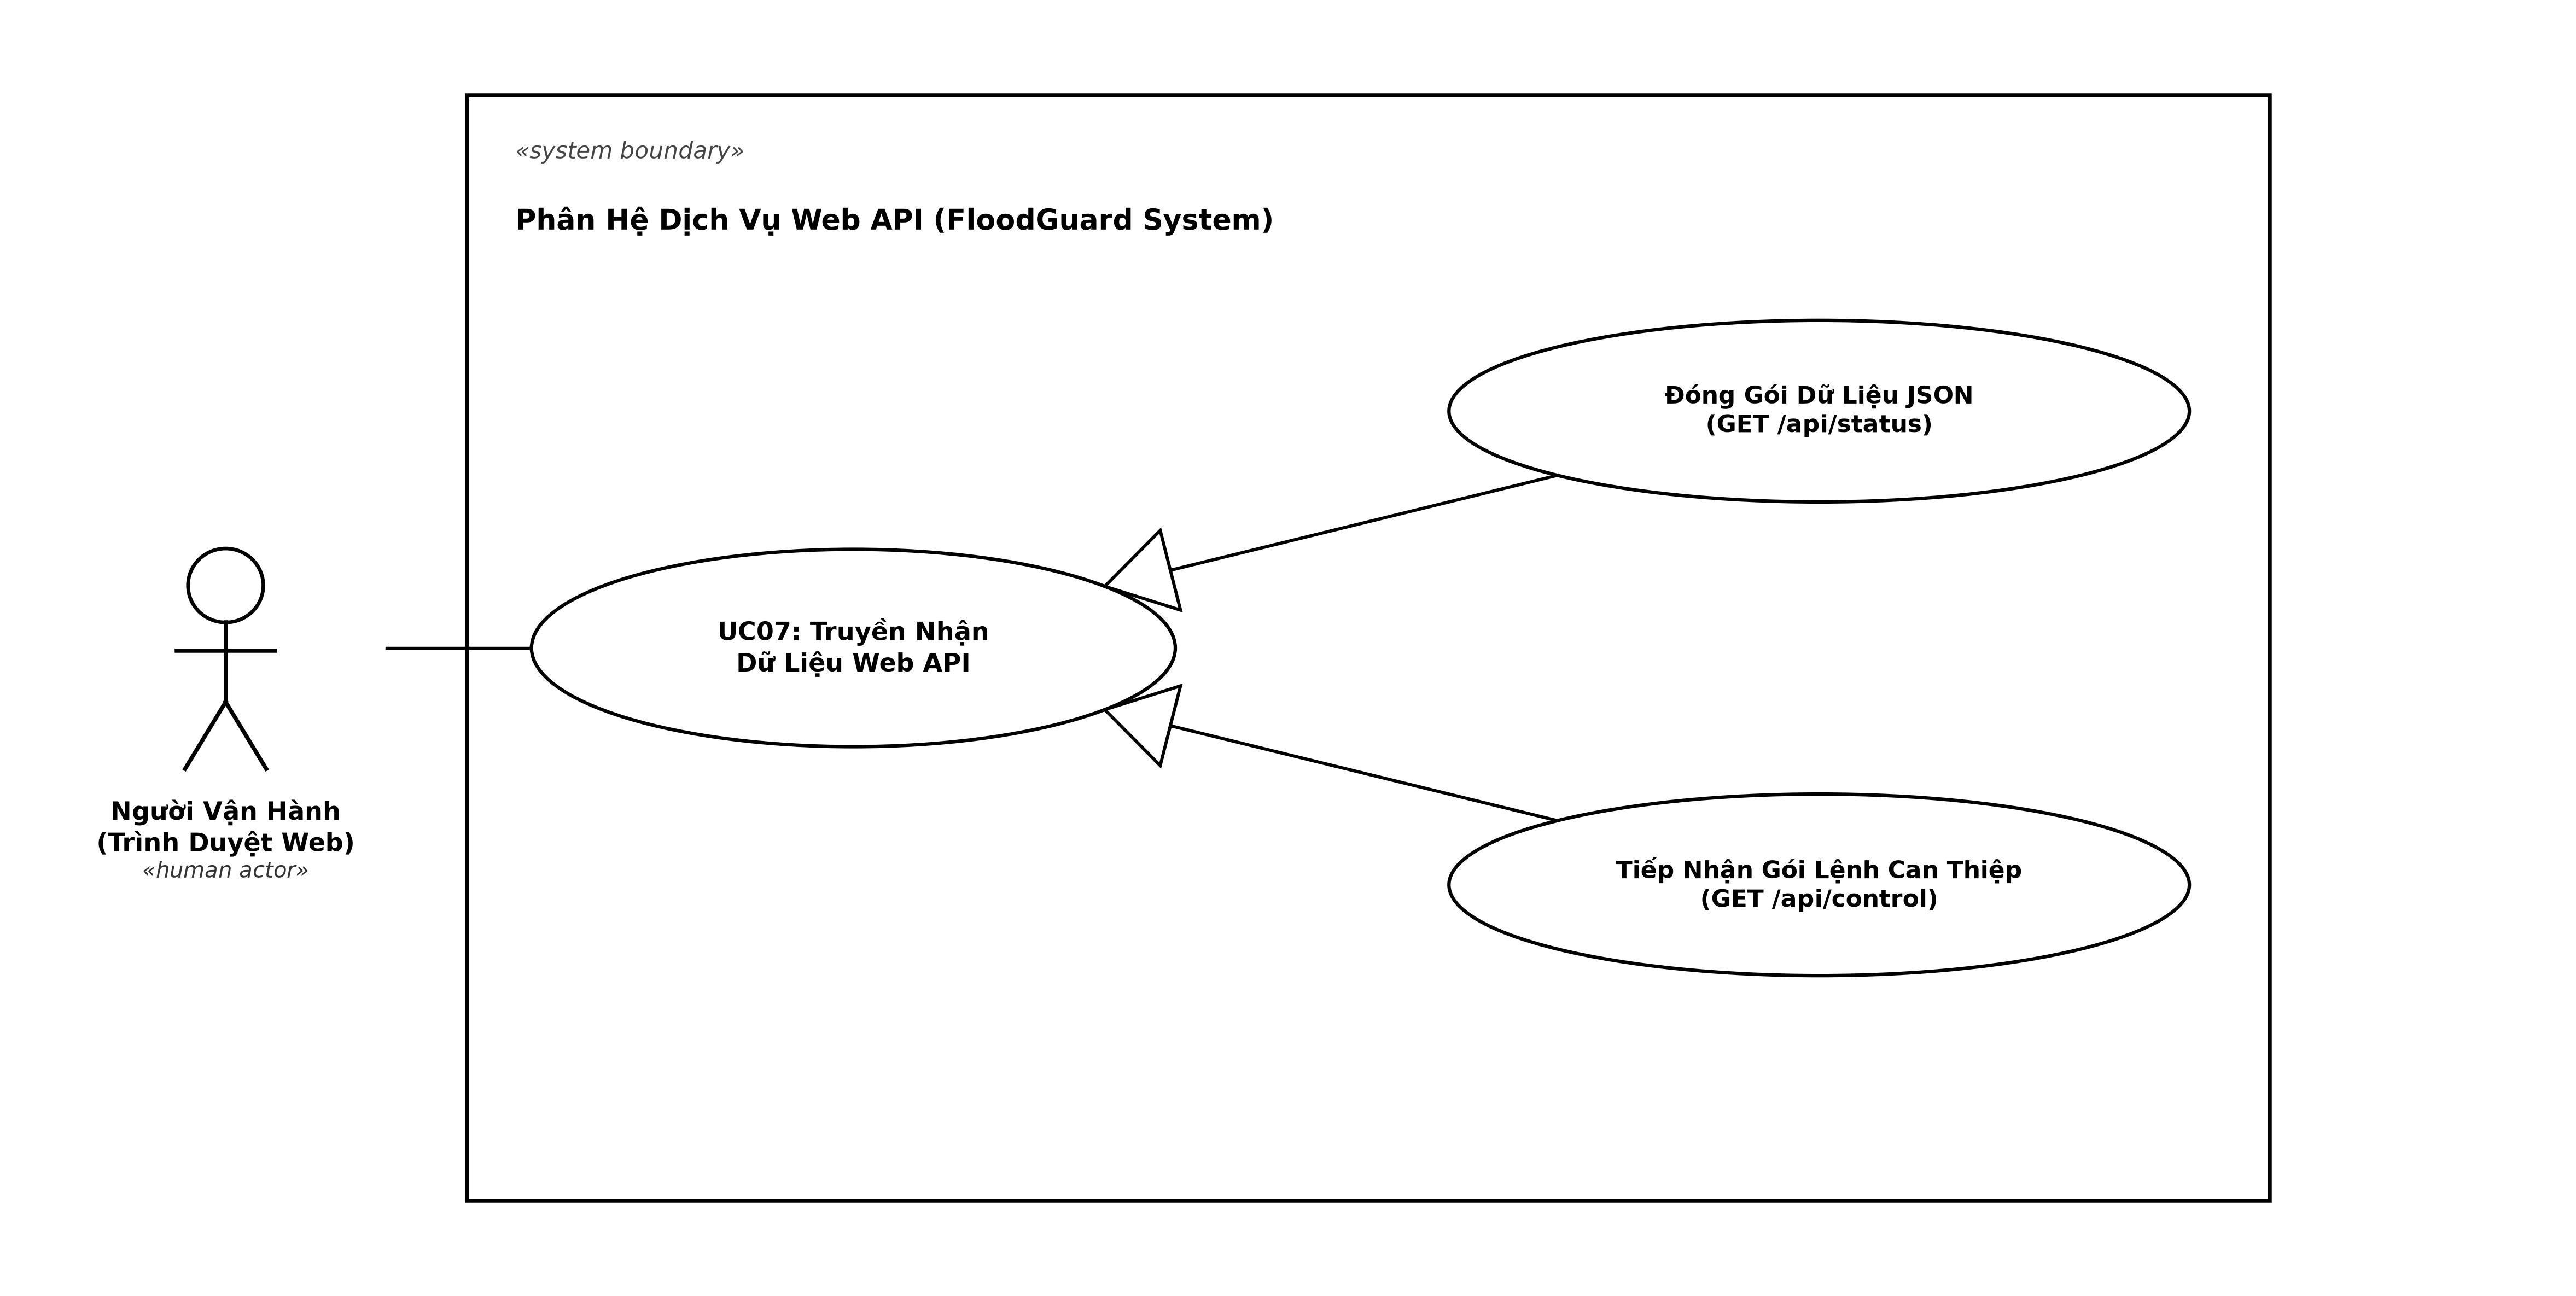
\includegraphics[width=0.88\textwidth]{figures/uc07_telemetry_api.png}
    \caption{Sơ đồ tương tác tác nhân UC07: Truyền nhận dữ liệu thời gian thực qua Web API}
    \label{fig:uc07}
\end{figure}

% --- UC08 ---
\subsubsection{UC08: Giám Sát Trạng Thái Trạm Từ Xa Trên Giao Diện Web}
\begin{itemize}
    \item \textbf{Mã định danh:} \texttt{UC08}
    \item \textbf{Tác nhân:}
    \begin{itemize}
        \item \textit{Con người:} Người giám sát / Kỹ thuật viên vận hành trạm.
        \item \textit{Phần mềm:} Trình duyệt Web (Chrome, Edge, Safari) đóng vai trò Dashboard SPA.
    \end{itemize}
    \item \textbf{Mục tiêu:} Hiển thị trực quan dữ liệu đo đạc và trạng thái phần cứng trên máy tính/điện thoại mà không cần màn hình LCD vật lý tại trạm.
    \item \textbf{Tiền điều kiện:} Thiết bị người dùng đã kết nối vào mạng Wi-Fi của trạm (\texttt{FloodGuard\_AP}) hoặc cùng Router Wi-Fi.
    \item \textbf{Luồng sự kiện chính:}
    \begin{enumerate}
        \item Người dùng mở trình duyệt, truy cập địa chỉ IP của ESP32 (ví dụ: \texttt{http://192.168.4.1}).
        \item Trình duyệt tải giao diện Dark Glassmorphism và kích hoạt JavaScript \texttt{fetch('/api/status')} định kỳ mỗi \textbf{1 giây} (Single Page Application -- SPA).
        \item Giao diện tự động cập nhật động:
        \begin{itemize}
            \item Đồng hồ/Thanh tiến trình đo mực nước (\%) và khoảng cách (cm).
            \item Badge trạng thái hệ thống: NORMAL (Xanh), WARNING (Vàng), DANGER (Cam), CRITICAL (Đỏ nhấp nháy).
            \item Chỉ số cảm biến mưa: Khô ráo, Mưa nhỏ, Mưa to, Ngập nước.
            \item Trạng thái thiết bị: Bơm ON/OFF, Van $0\%/50\%/100\%$, Còi báo động.
        \end{itemize}
    \end{enumerate}
    \item \textbf{Hậu điều kiện:} Người dùng nắm bắt toàn diện diễn biến thời gian thực của trạm từ xa.
\end{itemize}

\begin{figure}[H]
    \centering
    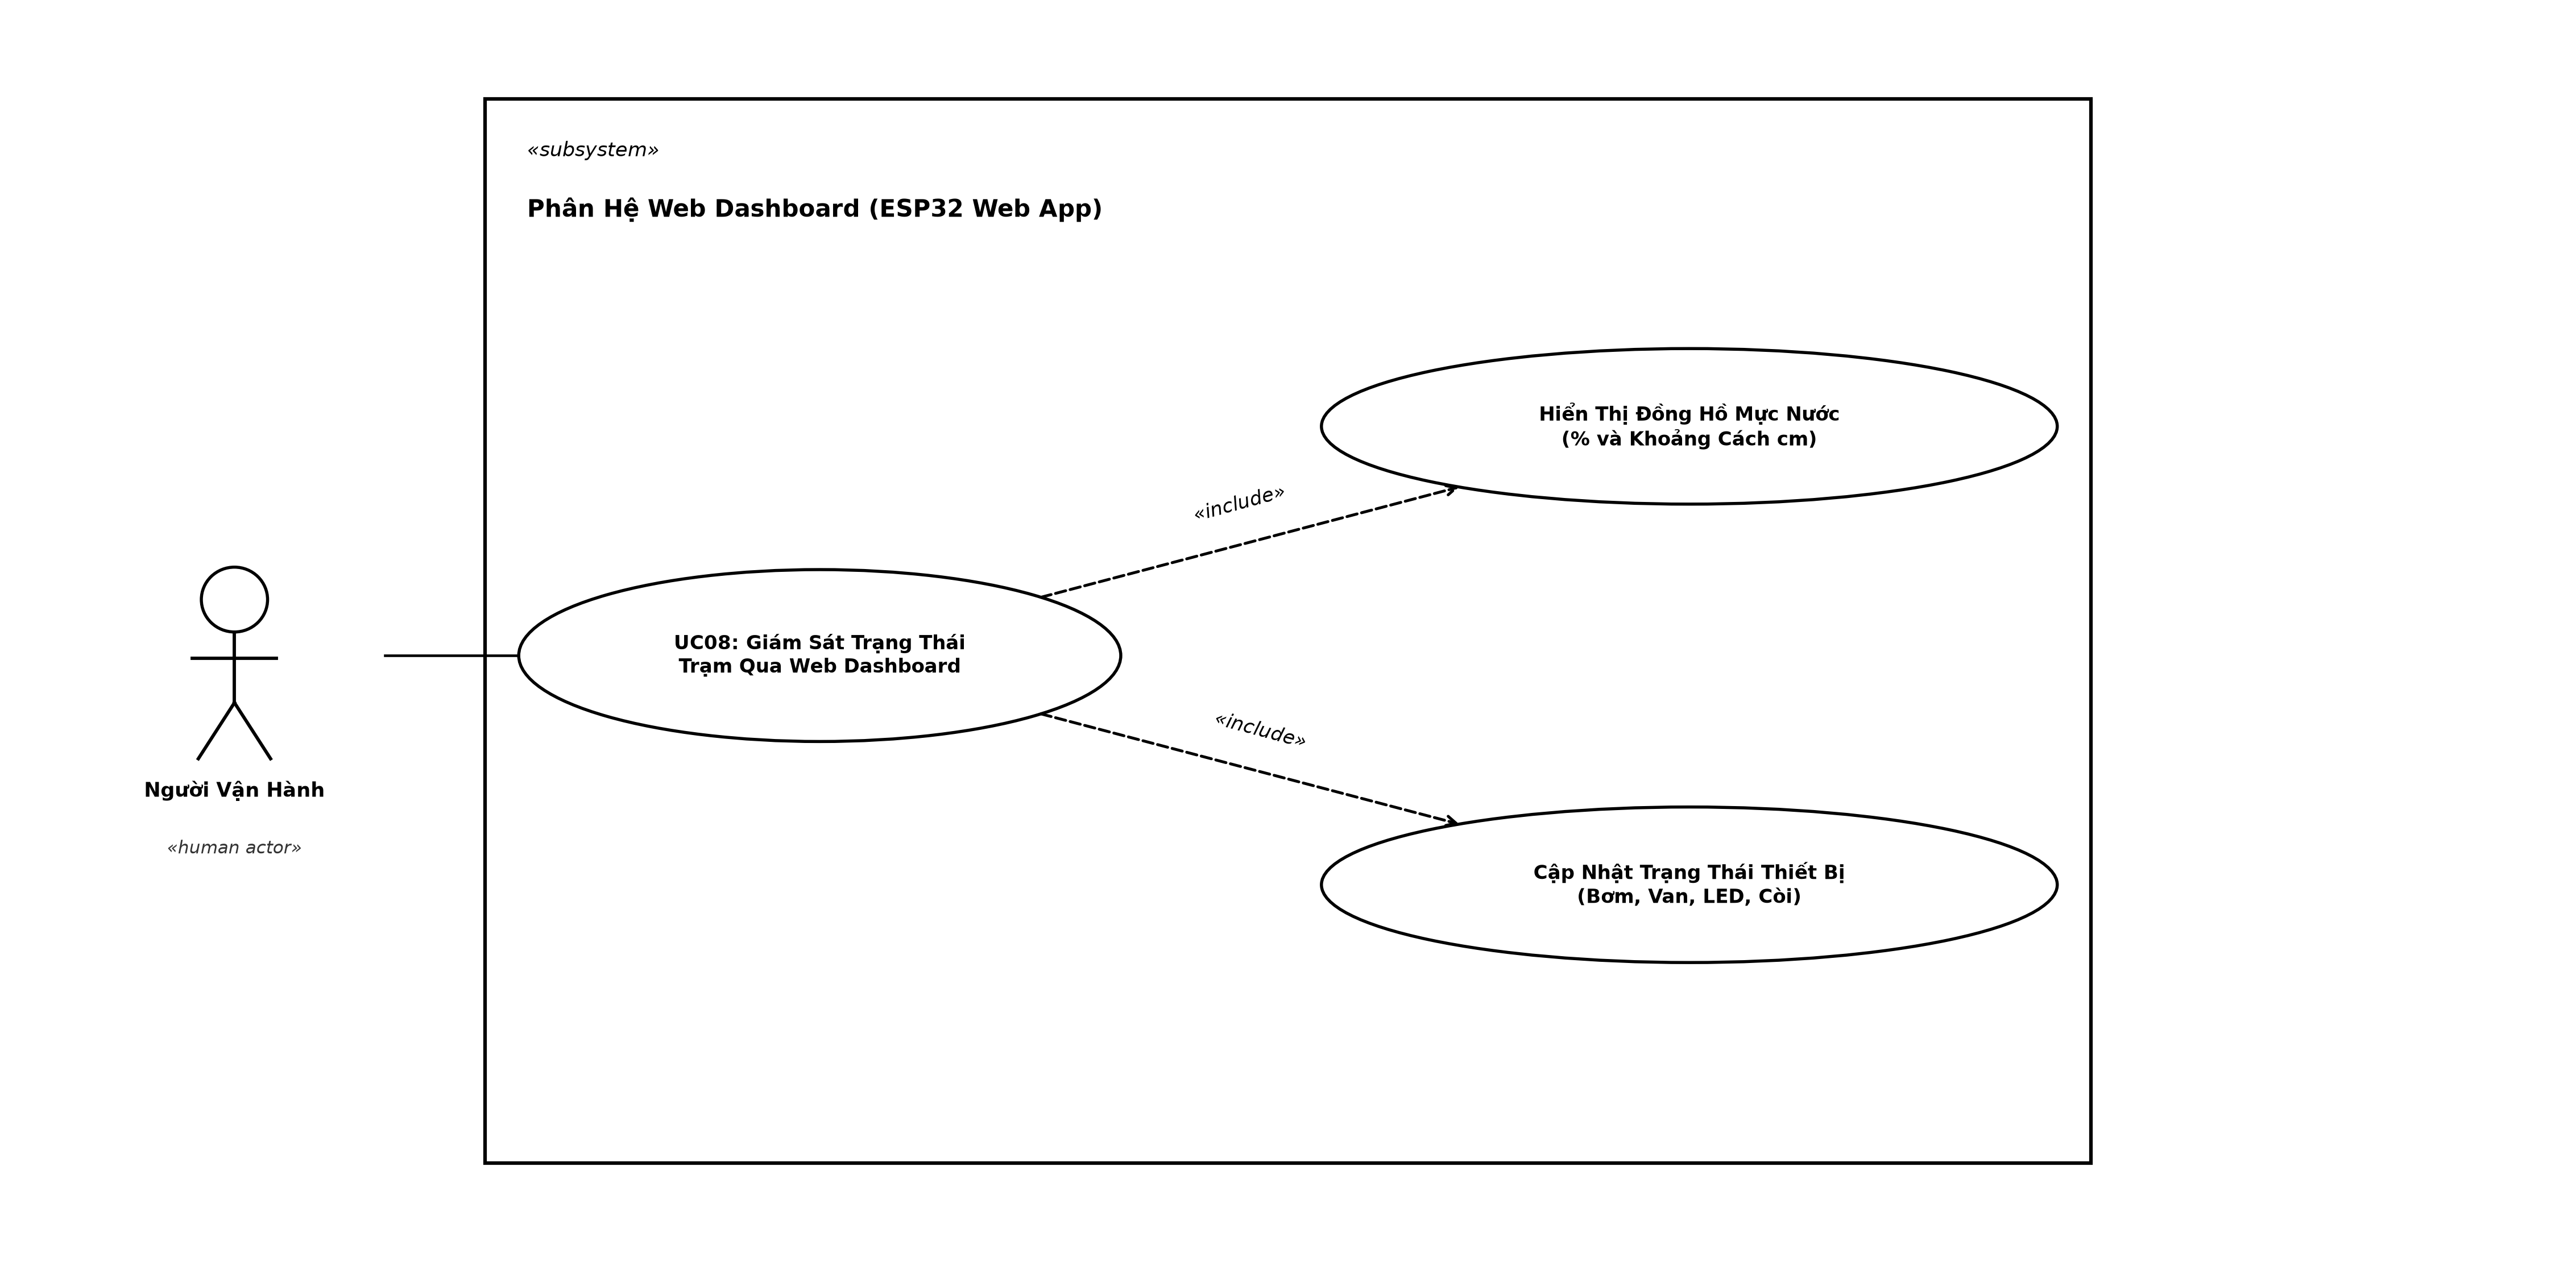
\includegraphics[width=0.88\textwidth]{figures/uc08_web_dashboard.png}
    \caption{Sơ đồ tương tác tác nhân UC08: Giám sát trạng thái trạm từ xa trên Web Dashboard}
    \label{fig:uc08}
\end{figure}

% --- UC09 ---
\subsubsection{UC09: Chuyển Đổi Chế Độ Vận Hành Từ Xa (AUTO / MANUAL)}
\begin{itemize}
    \item \textbf{Mã định danh:} \texttt{UC09}
    \item \textbf{Tác nhân:}
    \begin{itemize}
        \item \textit{Con người:} Kỹ thuật viên vận hành.
        \item \textit{Phần mềm \& Phần cứng:} Trình duyệt Web, ESP32 Controller.
    \end{itemize}
    \item \textbf{Mục tiêu:} Phân quyền điều khiển linh hoạt giữa thuật toán tự động thông minh và sự can thiệp thủ công của con người.
    \item \textbf{Tiền điều kiện:} Giao diện Web Dashboard đang kết nối bình thường với ESP32.
    \item \textbf{Luồng sự kiện chính:}
    \begin{enumerate}
        \item Người dùng nhấn nút \textbf{"Đổi Chế Độ (AUTO / MANUAL)"} trên Dashboard.
        \item Trình duyệt gửi request ngầm: \texttt{GET /api/control?action=mode\_toggle}.
        \item ESP32 tiếp nhận lệnh, đảo cờ trạng thái \texttt{isAutoMode = !isAutoMode}.
        \item Trình duyệt cập nhật badge hiển thị:
        \begin{itemize}
            \item \texttt{AUTO}: Khóa/vô hiệu hóa các nút điều khiển trực tiếp bơm/van để bảo vệ logic tự động.
            \item \texttt{MANUAL}: Mở khóa bảng điều khiển can thiệp thủ công (Manual Override).
        \end{itemize}
    \end{enumerate}
    \item \textbf{Hậu điều kiện:} Quyền điều khiển được chuyển giao an toàn giữa vi điều khiển và người dùng.
\end{itemize}

\begin{figure}[H]
    \centering
    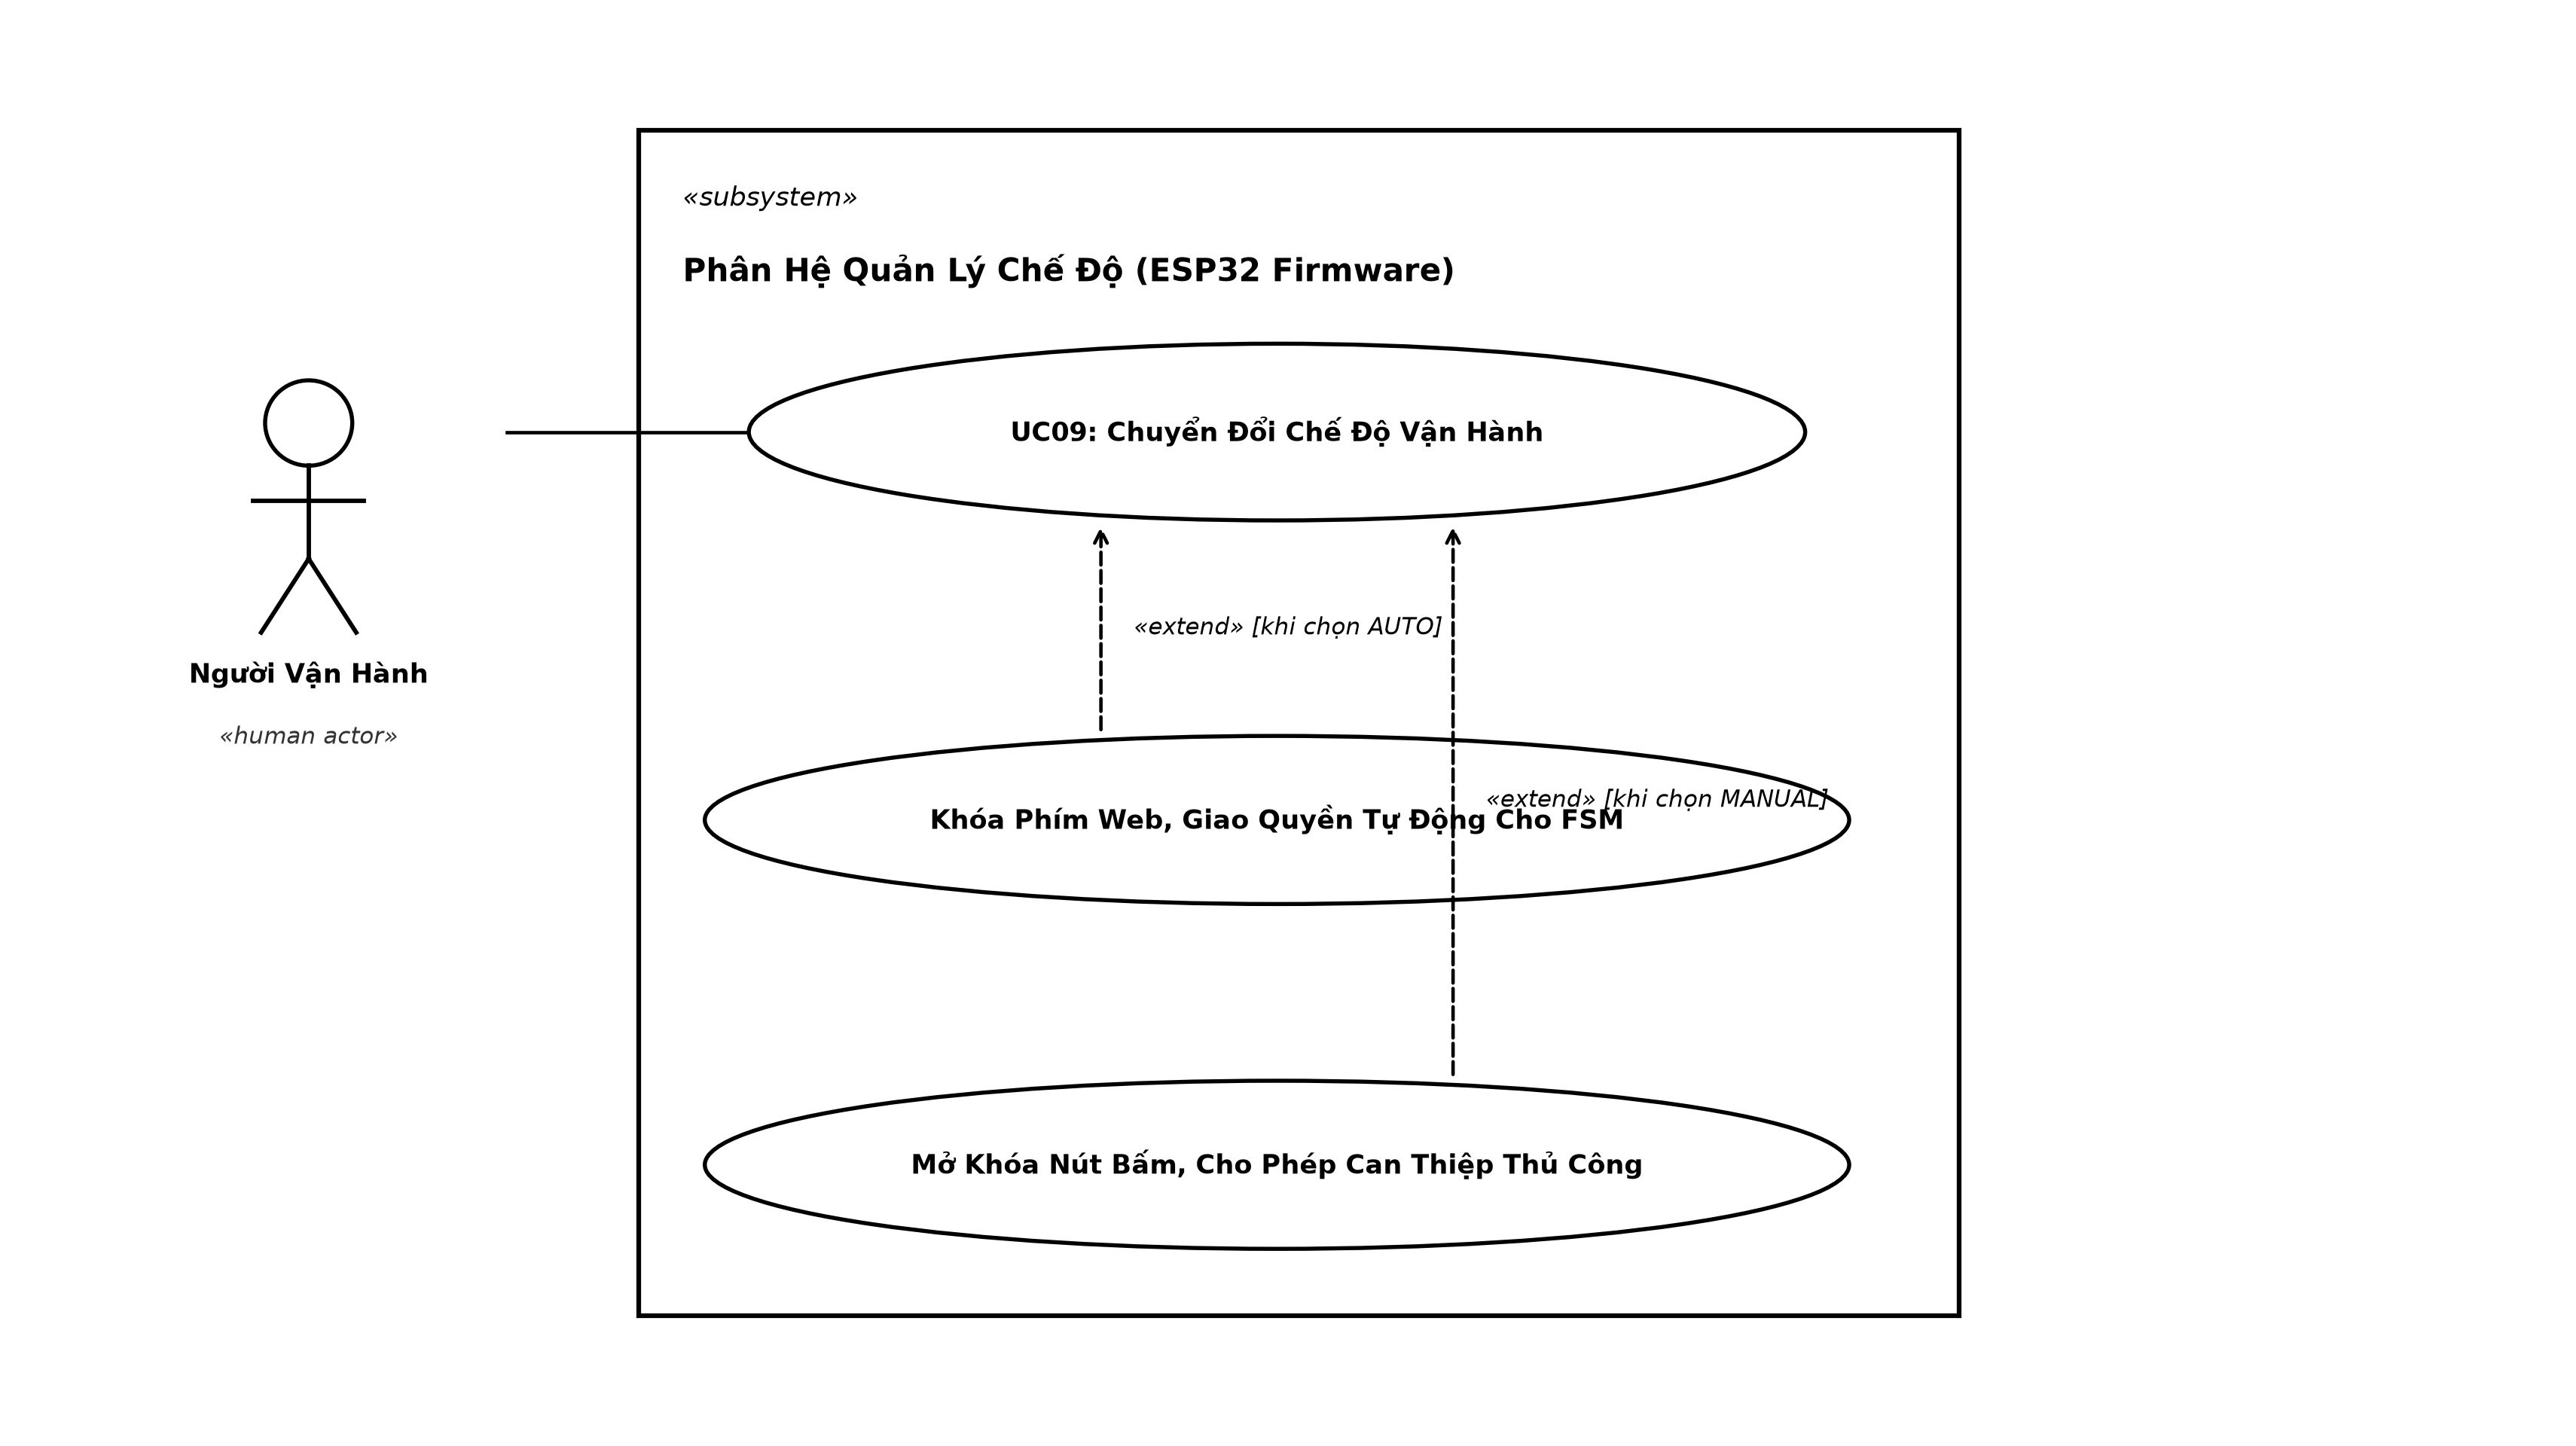
\includegraphics[width=0.88\textwidth]{figures/uc09_mode_switch.png}
    \caption{Sơ đồ tương tác tác nhân UC09: Chuyển đổi chế độ vận hành từ xa}
    \label{fig:uc09}
\end{figure}

% --- UC10 ---
\subsubsection{UC10: Điều Khiển Cưỡng Chế Thiết Bị Chấp Hành Từ Giao Diện Web}
\begin{itemize}
    \item \textbf{Mã định danh:} \texttt{UC10}
    \item \textbf{Tác nhân:}
    \begin{itemize}
        \item \textit{Con người:} Kỹ thuật viên vận hành.
        \item \textit{Vi điều khiển \& Chấp hành:} ESP32, Module Relay máy bơm, Động cơ Servo van xả.
    \end{itemize}
    \item \textbf{Mục tiêu:} Bật/tắt bơm hoặc xoay góc van xả thủ công phục vụ kiểm tra thiết bị định kỳ, xả cặn đáy hồ, hoặc xử lý sự cố khẩn cấp.
    \item \textbf{Tiền điều kiện:} Hệ thống đang ở chế độ \texttt{MANUAL MODE} (\texttt{isAutoMode == false}).
    \item \textbf{Luồng sự kiện chính:}
    \begin{enumerate}
        \item Người dùng nhấn các nút thao tác trên Dashboard Web:
        \begin{itemize}
            \item Nhấn \textbf{"Bật/Tắt Bơm (Manual)"}: Gửi lệnh \texttt{pump\_toggle}. ESP32 đảo trạng thái biến \texttt{pumpState} và kích hoạt Relay qua kỹ thuật High-Z.
            \item Nhấn \textbf{"Van 0\% (Đóng)"}, \textbf{"Van 50\% (Mở Nửa)"}, hoặc \textbf{"Van 100\% (Mở Hết)"}: Gửi lệnh tương ứng. ESP32 điều khiển Servo quay về $0^\circ, 90^\circ$, hoặc $180^\circ$.
        \end{itemize}
        \item ESP32 áp đặt đầu ra phần cứng ngay lập tức qua hàm \texttt{applyOutputs()}.
        \item Web Server trả về mã phản hồi \texttt{200 OK}, Dashboard cập nhật trạng thái thiết bị hiển thị lên màn hình.
    \end{enumerate}
    \item \textbf{Hậu điều kiện:} Thiết bị chấp hành vận hành chính xác theo ý muốn của người điều khiển bất chấp giá trị cảm biến hiện tại.
\end{itemize}

\begin{figure}[H]
    \centering
    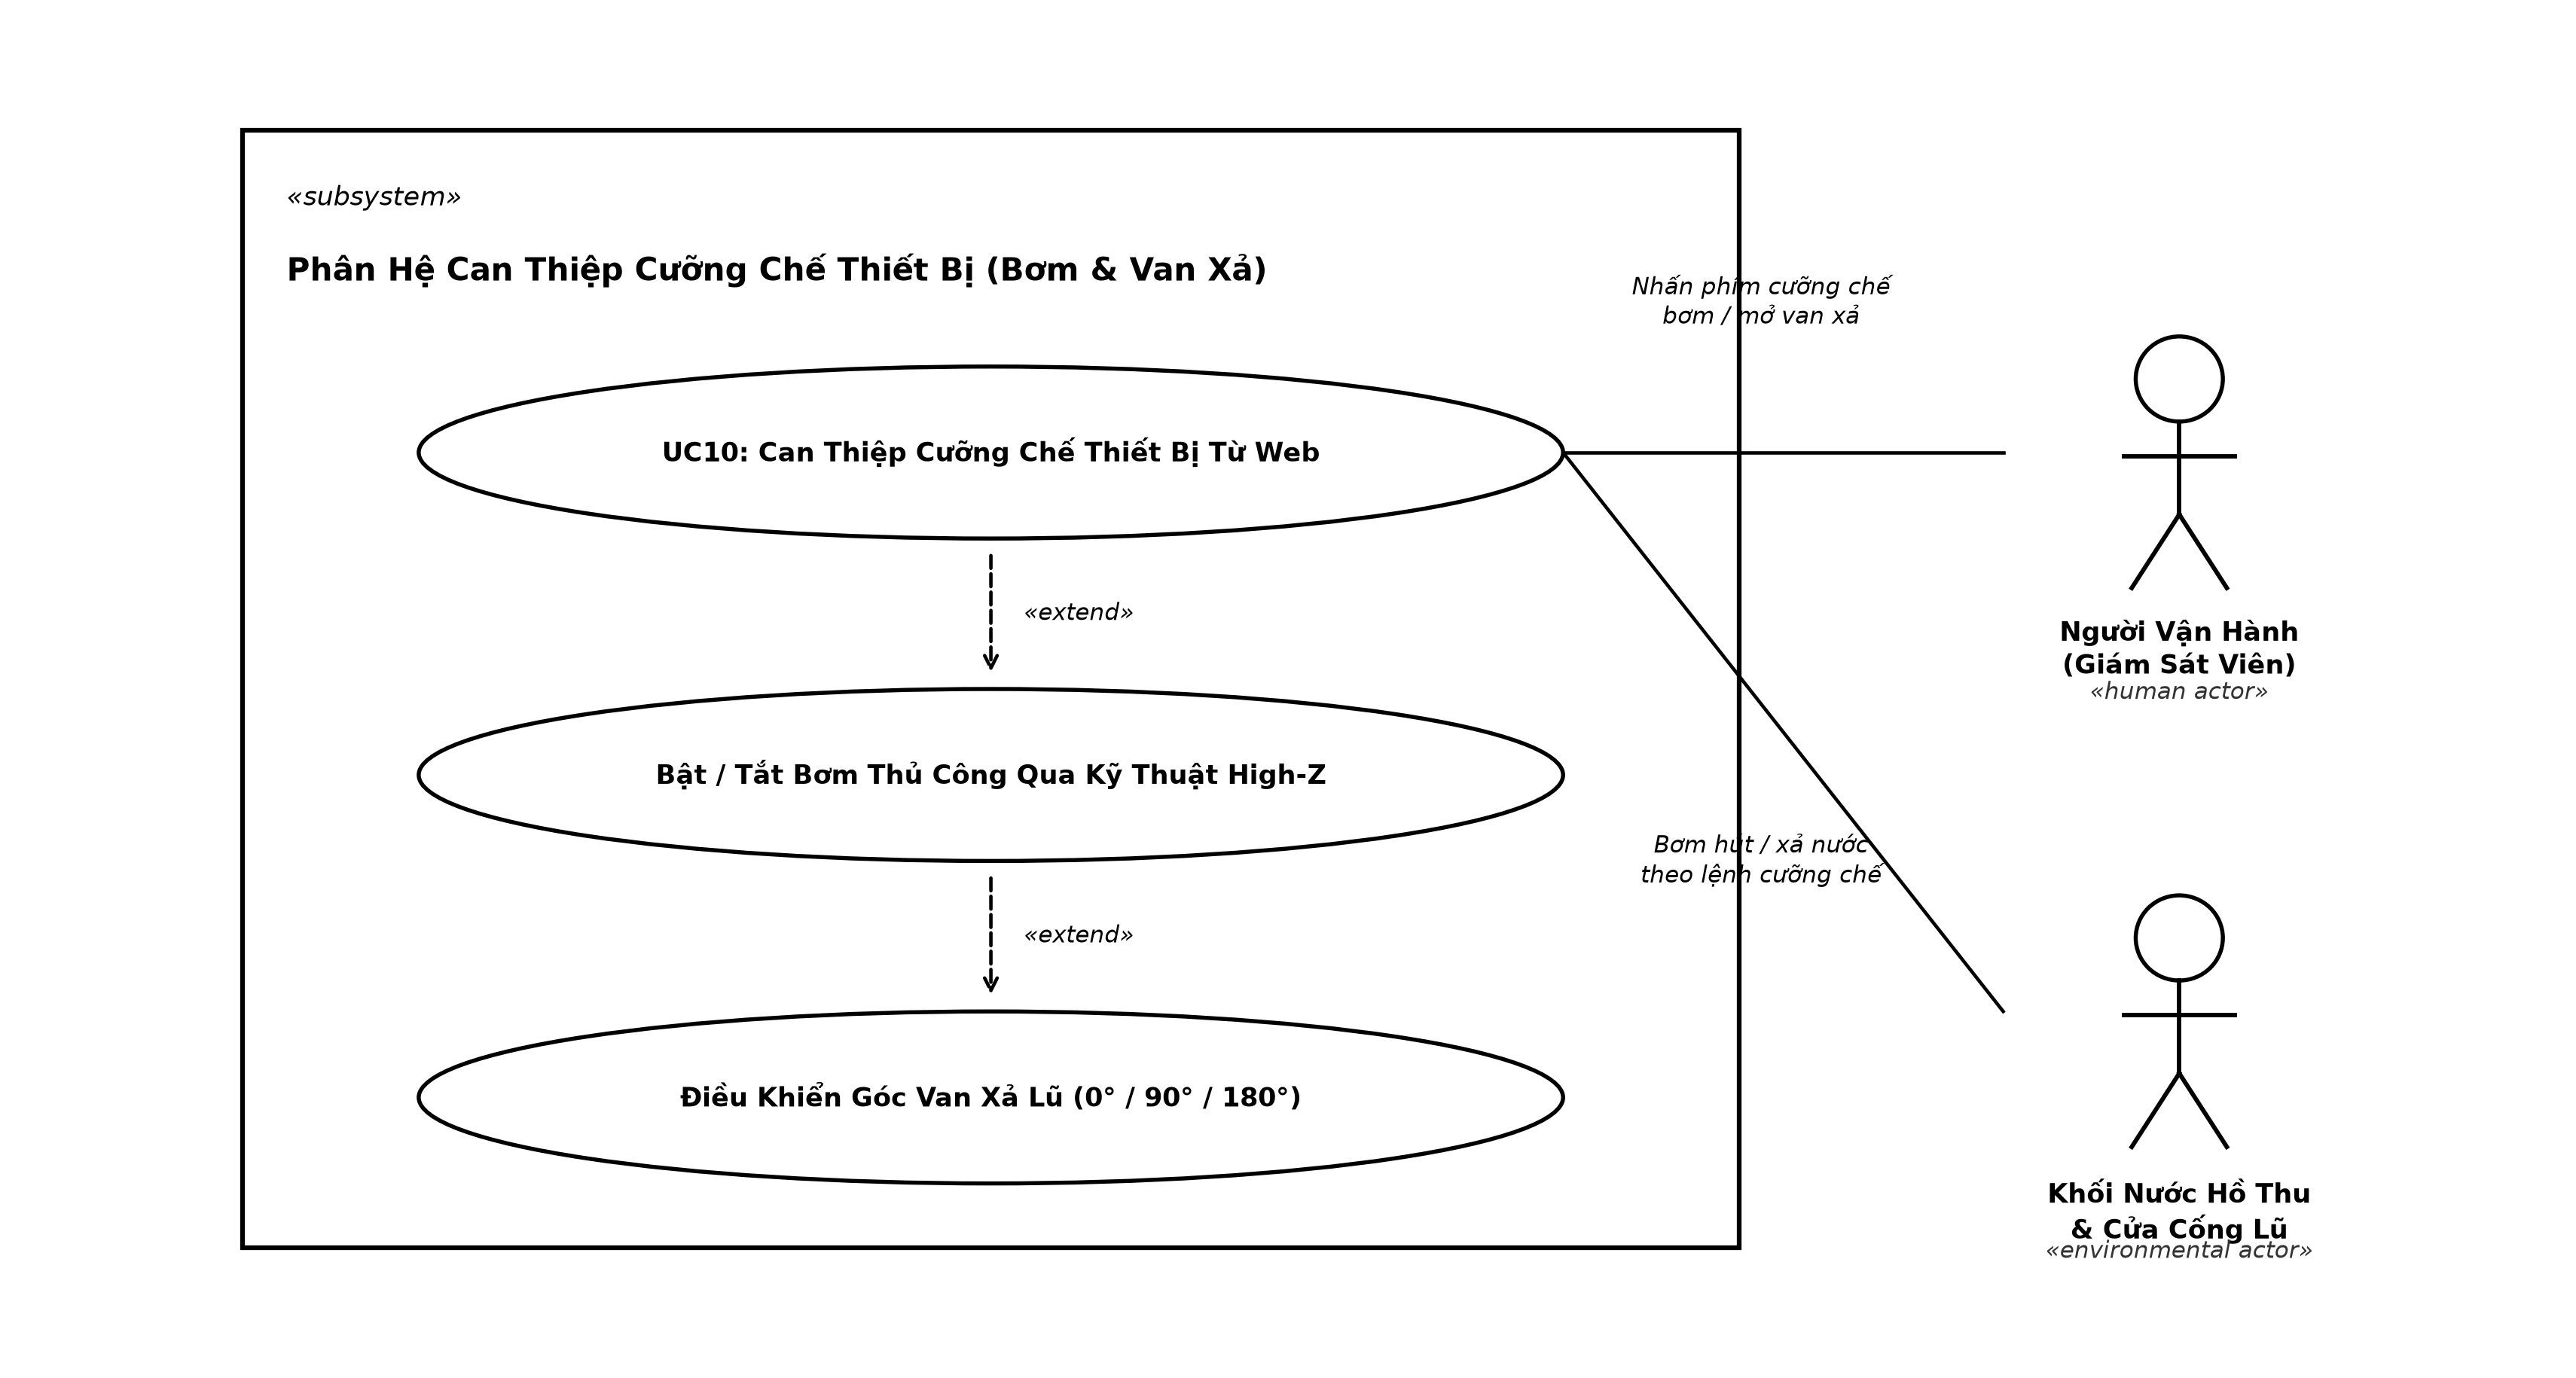
\includegraphics[width=0.88\textwidth]{figures/uc10_manual_override.png}
    \caption{Sơ đồ tương tác tác nhân UC10: Điều khiển cưỡng chế thiết bị chấp hành từ Web}
    \label{fig:uc10}
\end{figure}

\chapter{Thiết Kế và Lắp Đặt Hệ Thống}
\label{ch:hardware_architecture}

\section{Tổng Quan Kiến Trúc Hệ Thống}
Hệ thống FloodGuard gồm 5 khối chức năng chính được tích hợp đồng bộ:
\begin{enumerate}
    \item \textbf{Khối xử lý trung tâm:} Vi điều khiển ESP32 DevKit V1 với chip lõi kép Xtensa 32-bit (tần số xung nhịp $240\,\text{MHz}$), tích hợp bộ nhớ SRAM $520\,\text{KB}$ và kết nối không dây Wi-Fi $802.11\,\text{b/g/n}$, đảm nhiệm đồng thời tác vụ đo đạc thời gian thực, thuật toán FSM và máy chủ Web Server nhúng.
    \item \textbf{Khối cảm biến (Sensors):} Cảm biến siêu âm HC-SR04 đo khoảng cách tới mặt nước hồ thu và cảm biến mưa FC-37 (tấm điện cực kết hợp mạch so sánh LM393) đo lượng nước mưa bề mặt.
    \item \textbf{Khối chấp hành (Actuators):} Gồm hai cơ cấu chấp hành độc lập: Động cơ Servo SG90 điều khiển góc mở cửa van xả lũ ($0^\circ - 90^\circ - 180^\circ$) và Module Relay $5\,\text{V}$ điều khiển đóng/ngắt máy bơm mini thoát nước.
    \item \textbf{Khối cảnh báo tại chỗ (Signaling):} Cụm 3 đèn LED màu (Xanh, Vàng, Đỏ) và còi báo động Active Buzzer $5\,\text{V}$.
    \item \textbf{Khối máy tính vận hành (Operator PC/Laptop):} Trạm máy tính kết nối không dây qua sóng Wi-Fi SoftAP để mở giao diện Web Dashboard giám sát và can thiệp điều khiển; đồng thời kết nối có dây qua cổng Micro-USB phục vụ nạp firmware PlatformIO và theo dõi Serial Debug Monitor.
\end{enumerate}

\section{Giải Pháp Điều Khiển Qua Mạng Không Dây Cục Bộ Thay Cho Nút Nhấn Cơ Học}

Trong thiết kế trạm FloodGuard, giao diện giám sát và điều khiển can thiệp được chuyển dịch hoàn toàn sang \textbf{giao diện Web Dashboard thông qua mạng không dây cục bộ (Local Wi-Fi / SoftAP)} thay cho các nút bấm vật lý tại chỗ. Giải pháp này xuất phát từ các lập luận kỹ thuật và thực tiễn vận hành:
\begin{itemize}
    \item \textbf{Đảm bảo an toàn tính mạng cho người vận hành:} Mục tiêu cốt lõi của trạm bơm chống ngập là vận hành tự trị $24/7$. Khi xảy ra thiên tai mưa bão ngập lụt, khu vực hồ thu và trạm bơm tiềm ẩn nguy cơ giông sét đánh, sụt lở mép bờ và rò rỉ điện từ các đường dây động lực ngâm trong nước. Việc điều khiển không dây cho phép kỹ thuật viên đứng từ vị trí khô ráo an toàn (trong xe chỉ huy hoặc trên tầng cao tòa nhà cách trạm $15 - 30\,\text{m}$) để theo dõi và ra lệnh.
    \item \textbf{Cung cấp đầy đủ ngữ cảnh dữ liệu trước khi can thiệp:} Khác với nút bấm vật lý vốn chỉ cho phép thao tác "mù" mà không biết chính xác mực nước hay trạng thái van xả, Web Dashboard hiển thị toàn bộ đồ họa số hóa (phần trăm nước, khoảng cách cm, cấp độ mưa, trạng thái FSM). Người vận hành có đầy đủ cơ sở thông tin kỹ thuật trước khi quyết định kích hoạt máy bơm hoặc xoay van xả lũ.
    \item \textbf{Phân tích rủi ro \& Giải pháp Dừng khẩn cấp (Emergency Stop):}
    Việc không trang bị nút bấm cơ học đồng nghĩa với việc nếu thiết bị di động hết pin hoặc mạng Wi-Fi bị nhiễu sóng nặng, người tại chỗ không thể can thiệp tức thời. Để giảm thiểu rủi ro này:
    \begin{itemize}
        \item Trong mô hình thực nghiệm, hệ thống áp dụng cơ chế bảo vệ Failsafe tự động chuyển về \texttt{AUTO} sau $30\,\text{s}$ mất kết nối và tự động kích hoạt bơm toàn tải nếu nước chạm mức nguy cấp CRITICAL.
        \item Tuy nhiên, theo các tiêu chuẩn an toàn máy móc công nghiệp (ISO 13850 và IEC 60204-1), ở phiên bản sản xuất thương mại thực tế ngoài hiện trường, hệ thống khuyến nghị bắt buộc bố trí thêm \textbf{01 nút Dừng khẩn cấp cơ học (E-Stop Button)} dạng nấm màu đỏ có chốt khóa, đấu ngắt trực tiếp nguồn điện cấp cho cuộn hút Relay của máy bơm nhằm xử lý sự cố kẹt rác cơ học hoặc cháy nổ động cơ tại chỗ.
    \end{itemize}
\end{itemize}

\section{Bảng Phân Công Chân GPIO}
\begin{table}[H]
\centering
\caption{Bảng phân công chân phần cứng trên vi điều khiển ESP32}
\label{tab:gpio_mapping}
\begin{tabularx}{\textwidth}{c l l l X}
\toprule
\textbf{STT} & \textbf{Thiết bị / Module} & \textbf{Chân tín hiệu} & \textbf{GPIO ESP32} & \textbf{Chức năng kỹ thuật \& Lưu ý điện áp} \\
\midrule
1 & HC-SR04 (Siêu âm) & Trig & \texttt{GPIO 13} & Phát xung kích siêu âm $10\,\mu\text{s}$ ($3.3\,\text{V}$) \\
1 & HC-SR04 (Siêu âm) & Echo & \texttt{GPIO 12} & Nhận xung phản hồi (Strapping Pin MTDI; hạ áp $5\,\text{V} \to 3.3\,\text{V}$) \\
2 & Cảm biến mưa FC-37 & DO (Digital) & \texttt{GPIO 34} & Ngõ vào số báo mưa/khô (Input-only, không pull-up nội) \\
2 & Cảm biến mưa FC-37 & AO (Analog) & \texttt{GPIO 35} & Đo điện áp tương tự qua ADC1\_CH7 (Input-only) \\
3 & Động cơ Servo SG90 & PWM & \texttt{GPIO 27} & Xung PWM điều khiển van xả ($0^\circ - 90^\circ - 180^\circ$) \\
4 & Module Relay 5V & IN & \texttt{GPIO 23} & Kích đóng/ngắt máy bơm 5V -- \textbf{Active LOW} \\
5 & LED Đỏ (Nguy cấp) & Anode (+) & \texttt{GPIO 18} & Báo động CRITICAL / DANGER (nối tiếp $R = 220\,\Omega$) \\
6 & LED Vàng (Cảnh báo) & Anode (+) & \texttt{GPIO 19} & Báo trạng thái WARNING (nối tiếp $R = 220\,\Omega$) \\
7 & LED Xanh (An toàn) & Anode (+) & \texttt{GPIO 21} & Báo trạng thái NORMAL (nối tiếp $R = 220\,\Omega$) \\
8 & Còi Active Buzzer 5V & Cực (+) & \texttt{GPIO 4} & Phát xung âm thanh cảnh báo đa cấp độ \\
\bottomrule
\end{tabularx}
\end{table}

\section{Sơ Đồ Nguyên Lý Mạch Điện \& Kết Nối Ngoại Vi}

Sơ đồ nguyên lý mạch điện chi tiết kết nối giữa vi điều khiển ESP32 với toàn bộ cảm biến, cơ cấu chấp hành, thiết bị chỉ thị và máy tính vận hành được minh họa trong Hình~\ref{fig:circuit_diagram}.

\begin{figure}[H]
    \centering
    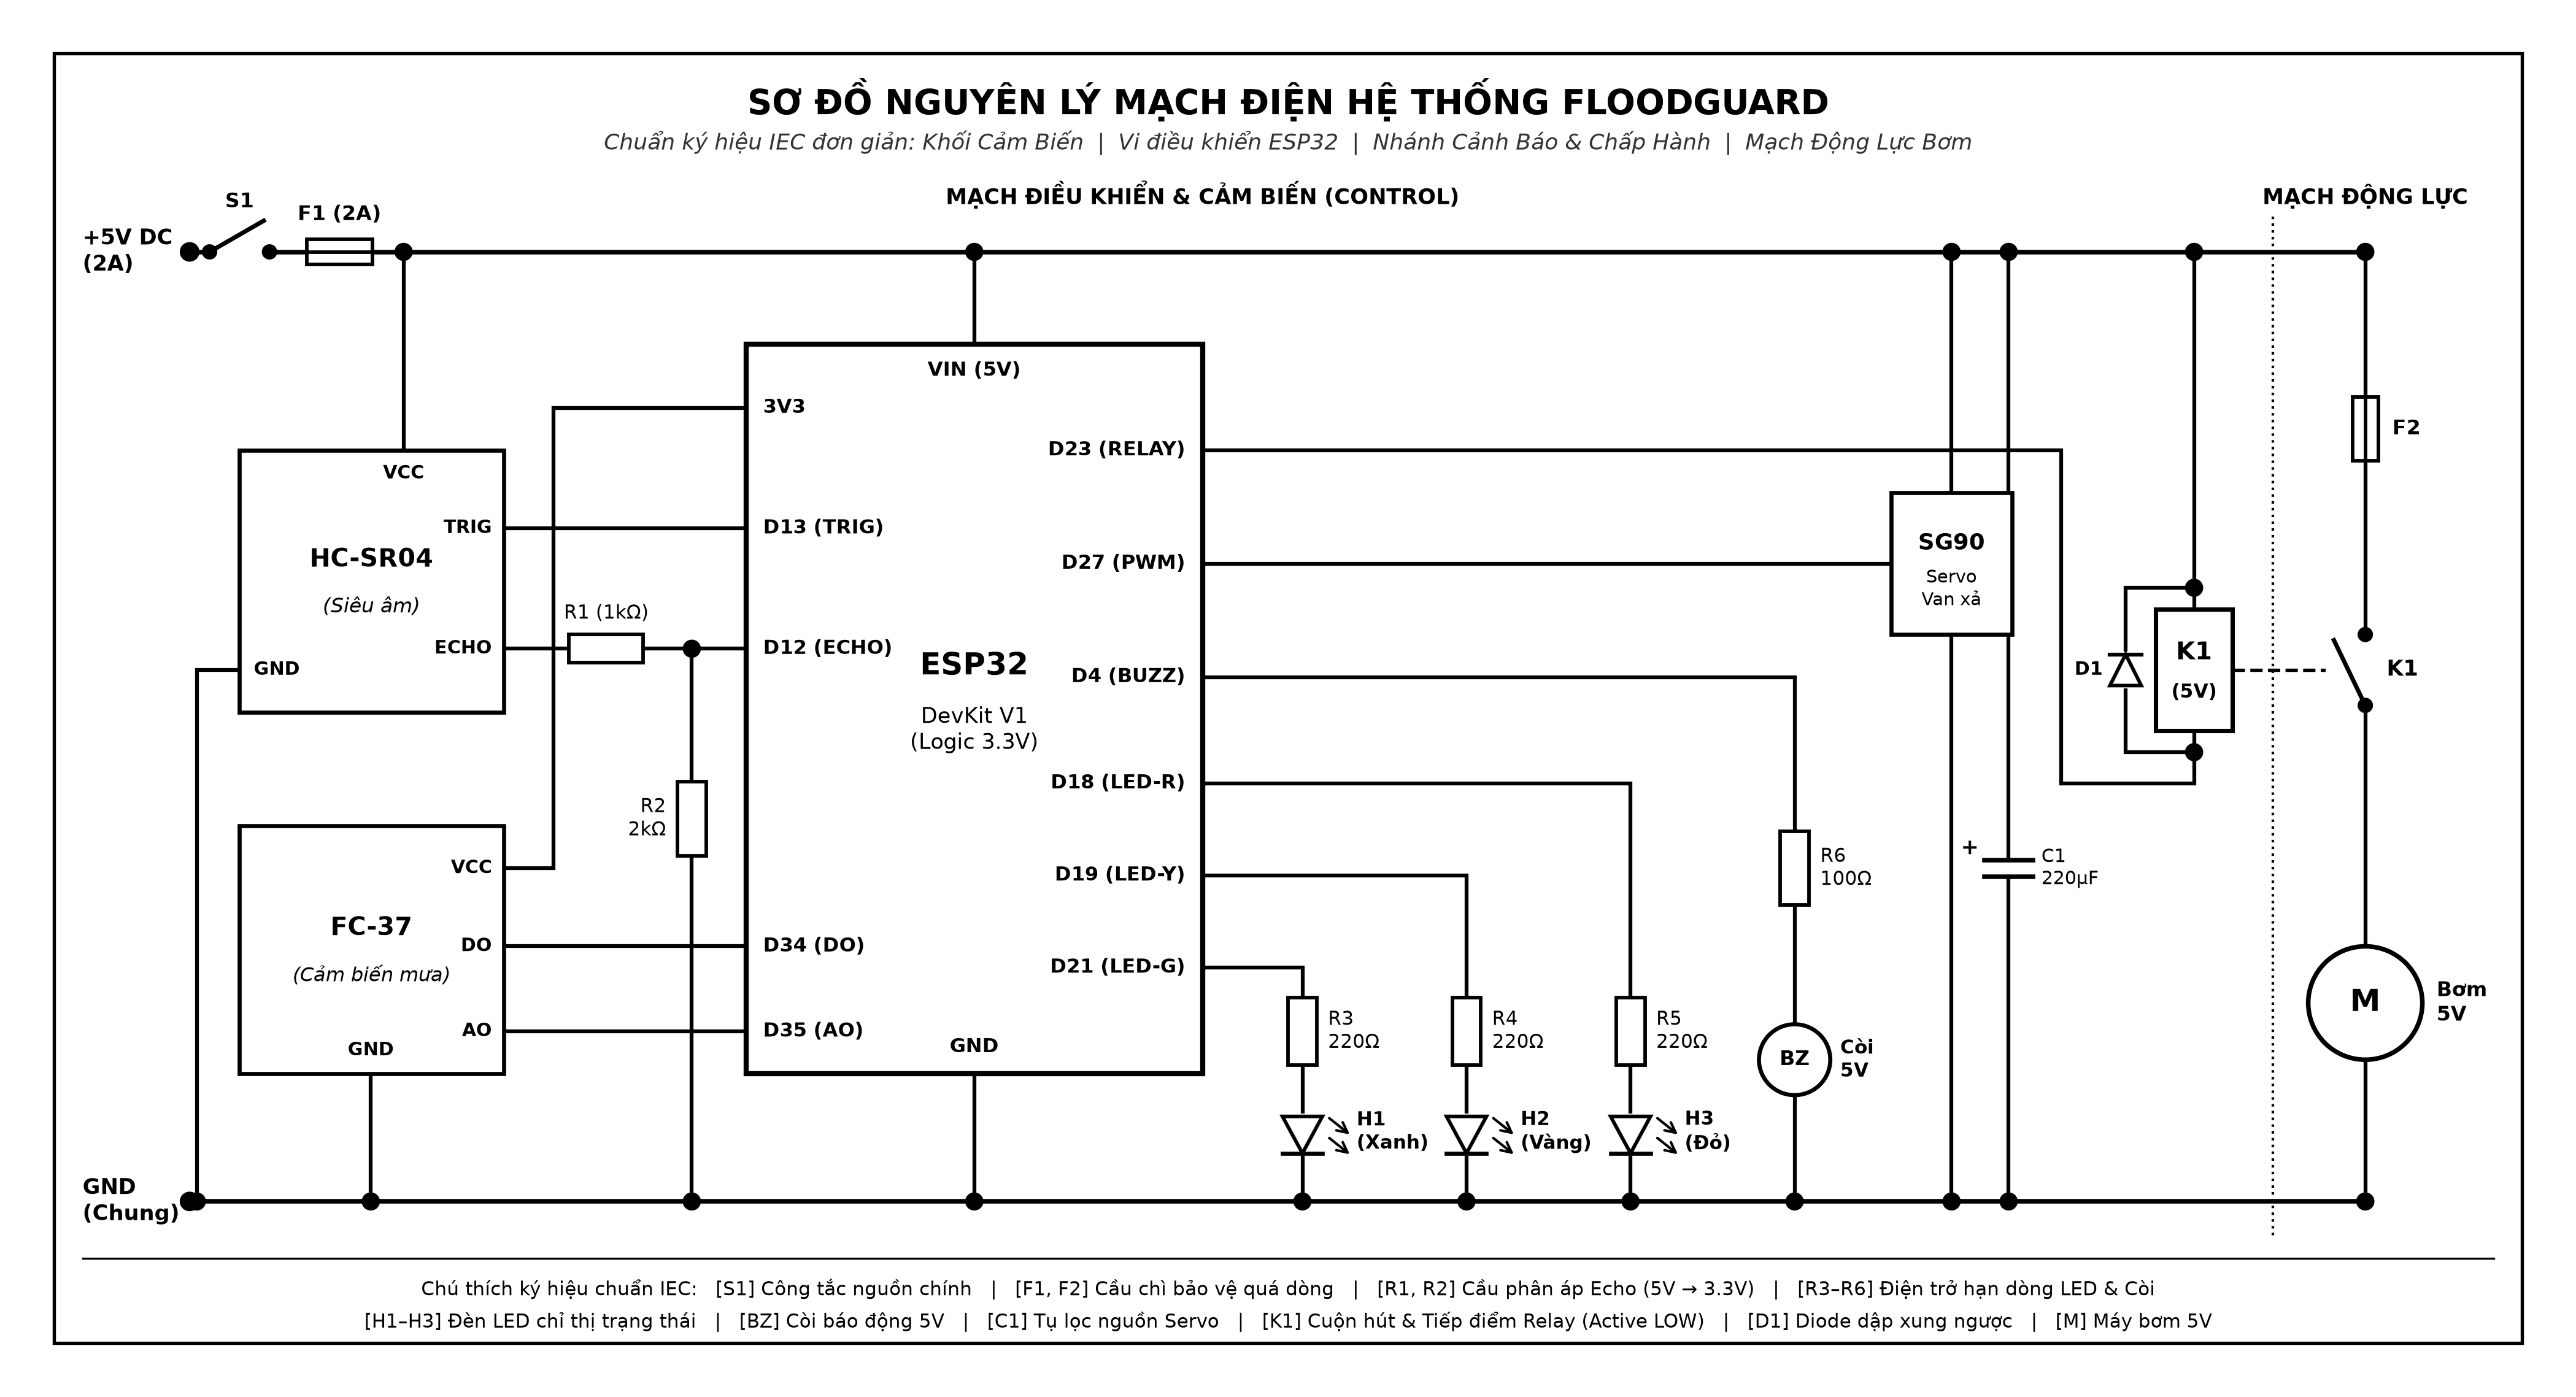
\includegraphics[width=\textwidth]{figures/circuit_diagram.png}
    \caption{Sơ đồ nguyên lý mạch điện chuẩn IEC và phân vùng các khối chấp hành trạm FloodGuard}
    \label{fig:circuit_diagram}
\end{figure}

Dựa trên sơ đồ nguyên lý nối dây và phân vùng các khối chấp hành, các nguyên lý phối ghép phần cứng và giải pháp bảo vệ mạch điện được phân tích chi tiết:

\subsection{Khối Chấp Hành Công Suất: Relay 5V, Diode Flyback \& Nguồn Cấp Máy Bơm}
Máy bơm nước mini $5\,\text{V}$ sử dụng động cơ DC có chổi than, tiêu thụ dòng điện làm việc định mức khoảng $0.5 - 0.8\,\text{A}$ và có thể lên tới $1.5\,\text{A}$ khi khởi động (\textit{Inrush current}). Để vận hành an toàn:
\begin{itemize}
    \item \textbf{Phân tách nguồn cấp động lực:} Nguồn cấp cho máy bơm được lấy từ chân \texttt{VIN} (nối với bộ nguồn $5\,\text{V} - 2\,\text{A}$ bên ngoài), tuyệt đối không lấy từ chân \texttt{3V3} của ESP32 nhằm tránh hiện tượng sụt áp gây khởi động lại vi điều khiển (\textit{Brown-out Reset}).
    \item \textbf{Bảo vệ cách ly quang (Optocoupler) \& Diode dập xung ngược (Flyback Diode):} Module Relay tích hợp optocoupler PC817 cách ly hoàn toàn điện áp $3.3\,\text{V}$ của vi điều khiển với cuộn hút $5\,\text{V}$. Cuộn hút Relay được mắc song song với một Diode dập xung ngược (\textit{Flyback Diode}) phân cực ngược để triệt tiêu sức điện động cảm ứng $e = -L\frac{di}{dt}$ sinh ra khi ngắt dòng điện cuộn dây, ngăn chặn xung điện áp cao đánh thủng transistor kích mở.
    \item \textbf{Cơ chế điều khiển Active LOW kết hợp trạng thái High-Z:}
    Module Relay đóng tiếp điểm khi chân tín hiệu \texttt{IN} được kéo xuống mức \texttt{LOW} ($0\,\text{V}$). Do vi điều khiển ESP32 chỉ xuất mức \texttt{HIGH} ở $3.3\,\text{V}$, sự chênh lệch $5\,\text{V} - 3.3\,\text{V} = 1.7\,\text{V}$ có thể làm rò dòng qua LED phát quang nội của optocoupler khiến Relay không nhả hoàn toàn. Hệ thống xử lý triệt để hiện tượng này bằng cách:
    \begin{itemize}
        \item Khi bật bơm: Cấu hình ngõ ra \texttt{OUTPUT} và kéo chân Relay xuống mức \texttt{LOW} ($0\,\text{V}$).
        \item Khi ngắt bơm: Cấu hình ngõ vào \texttt{INPUT} thả nổi chân về trạng thái trở kháng cao (High-Z).
    \end{itemize}
\end{itemize}

\subsection{Khối Cảm Biến: Bảo Vệ Điện Áp Echo \& Chân Strapping GPIO 12}
\begin{itemize}
    \item \textbf{Cảm biến siêu âm HC-SR04 (GPIO 13 Trig, GPIO 12 Echo):}
    Cảm biến HC-SR04 sử dụng nguồn cấp $5\,\text{V}$. Chân \texttt{Echo} xuất ra xung vuông mức biên độ $5\,\text{V}$. Do các chân GPIO của ESP32 chỉ dung nạp điện áp tối đa $3.3\,\text{V}$, chân \texttt{Echo} được mắc qua mạch phân áp trở hoặc điện trở hạn dòng bảo vệ kết hợp diode kẹp áp nội của vi điều khiển để hạ mức điện áp an toàn xuống $\approx 3.3\,\text{V}$. Về mặt vật lý lắp đặt, cảm biến có vùng mù ở khoảng cách $< 3\,\text{cm}$ và góc phát chùm tia hình nón $\pm 15^\circ$; do đó khi gá đặt trên mô hình thực nghiệm, mặt loa cần đặt cao hơn mức nước đầy tối đa ít nhất $5 - 6\,\text{cm}$ và chiếu thẳng vào tâm bể để tránh dội sóng nhiễu vào thành bể.
    \item \textbf{Lưu ý kỹ thuật đặc biệt với chân Strapping MTDI (GPIO 12):}
    Trên vi điều khiển ESP32, \texttt{GPIO 12} là chân cấu hình khởi động (\textit{Strapping Pin MTDI}). Tại thời điểm cấp nguồn/reset, chip sẽ đọc mức logic của chân này: nếu ở mức \texttt{LOW}, chip chọn điện áp cấp cho bộ nhớ SPI Flash nội là $3.3\,\text{V}$ (bình thường); nếu bị kéo lên mức \texttt{HIGH}, chip chuyển sang chế độ Flash $1.8\,\text{V}$ dẫn tới treo vi điều khiển (vòng lặp Boot loop). Trong mạch thiết kế, chân \texttt{Echo} của cảm biến HC-SR04 ở trạng thái nghỉ luôn duy trì mức \texttt{LOW} ($0\,\text{V}$), do đó hoàn toàn an toàn và không cản trở quá trình khởi động bình thường của ESP32.
    \item \textbf{Cảm biến mưa FC-37 (GPIO 34 DO, GPIO 35 AO):}
    Module sử dụng nguồn $3.3\,\text{V}$. Chân \texttt{GPIO 34} và \texttt{GPIO 35} đều thuộc nhóm chân chỉ đọc (\textit{Input-only}) của ESP32, không tích hợp điện trở kéo nội (\textit{Internal Pull-up/Pull-down}). Trên module thương mại FC-37, bo mạch so sánh LM393 đã tích hợp sẵn điện trở kéo lên $10\,\text{k}\Omega$ cho chân ngõ ra số DO và mạch phân áp cho AO. Tuy nhiên, nếu cáp tín hiệu từ module về ESP32 bị tuột hoặc hở mạch, chân GPIO 35 thả nổi (\textit{floating}) có thể đọc ra điện áp thấp do điện dung ký sinh, dẫn tới nguy cơ thuật toán nhận diện nhầm là ngập cảm biến (\texttt{isSubmerged}). Do đó, thiết kế phần cứng khuyến nghị lắp thêm một điện trở kéo ngoại $100\,\text{k}\Omega$ lên $3.3\,\text{V}$ trực tiếp tại chân GPIO 35 để đảm bảo an toàn phần cứng (\textit{Hardware Failsafe}).
\end{itemize}

\subsection{Khối Động Cơ Servo SG90 (GPIO 27)}
Động cơ Servo SG90 điều khiển cửa van xả lũ nhận xung điều khiển PWM từ chân \texttt{GPIO 27} với tần số cơ sở $50\,\text{Hz}$ (chu kỳ $20\,\text{ms}$). Độ rộng xung điều khiển được ánh xạ tương ứng: $1.0\,\text{ms}$ ($0^\circ$ -- Đóng kín), $1.5\,\text{ms}$ ($90^\circ$ -- Mở $50\%$) và $2.0\,\text{ms}$ ($180^\circ$ -- Mở $100\%$). Nguồn nuôi Servo được cấp trực tiếp từ đường nguồn $5\,\text{V}$ (VIN) nhằm đảm bảo đủ mô-men xoắn kéo cửa van.

\subsection{Khối Thiết Bị Chỉ Thị \& Cảnh Báo Tại Trạm}
\begin{itemize}
    \item \textbf{Cụm 3 đèn LED phân cấp:} Gồm LED Đỏ (\texttt{GPIO 18}), LED Vàng (\texttt{GPIO 19}) và LED Xanh (\texttt{GPIO 21}). Mỗi đèn LED được mắc nối tiếp với điện trở hạn dòng $R = 220\,\Omega$. Tại điện áp ngõ ra $V_{\text{OH}} = 3.3\,\text{V}$, dòng điện định mức qua diode được xác định theo định luật Ohm:
    \begin{equation}
        I_{\text{LED}} = \frac{V_{\text{OH}} - V_f}{R} \approx \frac{3.3\,\text{V} - 2.0\,\text{V}}{220\,\Omega} \approx 5.9\,\text{mA}
    \end{equation}
    Dòng điện này nằm hoàn toàn trong dải tải làm việc khuyến nghị an toàn của GPIO ESP32 ($I_{\text{source}} \le 12\,\text{mA}$), đồng thời đảm bảo cường độ sáng rõ nét tại thực địa.
    \item \textbf{Còi báo động Active Buzzer 5V (GPIO 4):} Còi tích hợp sẵn mạch tạo dao động âm thanh bên trong với tần số cộng hưởng cố định $\approx 2.3\,\text{kHz}$ (do đó không cần và không thể dùng hàm \texttt{tone()} để đổi tần số như còi thụ động Passive Buzzer). Cực dương của còi được cấp nguồn và điều khiển đóng/ngắt logic từ \texttt{GPIO 4} qua trở hạn dòng đệm $100\,\Omega$. Thuật toán điều khiển sử dụng bộ đếm thời gian phi chặn \texttt{millis()}, băm xung bật/tắt (HIGH/LOW) theo các nhịp cảnh báo xác định mà không chiếm dụng chu kỳ CPU hay gây gián đoạn luồng đo cảm biến và máy chủ Web.
\end{itemize}

\subsection{Khối Máy Tính Vận Hành: Giao Tiếp Wi-Fi SoftAP \& Cáp USB PlatformIO}
Trên sơ đồ nguyên lý mạch điện (Hình~\ref{fig:circuit_diagram}), khối máy tính vận hành (PC / Laptop) đóng vai trò là trạm điều hành giám sát trung tâm và công cụ nạp mã nguồn bảo trì hệ thống. Máy tính tương tác trực tiếp với vi điều khiển ESP32 thông qua hai kênh truyền thông vật lý và logic độc lập:

\begin{itemize}
    \item \textbf{Kênh truyền thông không dây (Wi-Fi 2.4 GHz SoftAP):}
    \begin{itemize}
        \item \textit{Phương thức kết nối:} Vi điều khiển ESP32 khởi tạo một điểm truy cập không dây cục bộ (SoftAP) độc lập với SSID \texttt{FloodGuard\_AP}, bảo mật WPA2-PSK và cấp phát địa chỉ IP tự động cho máy tính qua giao thức DHCP nội bộ.
        \item \textit{Giao thức truyền tải:} Máy tính mở trình duyệt Web kết nối tới địa chỉ IP tĩnh của trạm \texttt{192.168.4.1} (hoặc tên miền \texttt{http://floodguard.local} qua mDNS). Dữ liệu giám sát telemetry được cập nhật định kỳ mỗi $1000\,\text{ms}$ qua endpoint \texttt{/api/status} với payload JSON $\approx 210\,\text{byte}$.
        \item \textit{Can thiệp điều khiển:} Khi người vận hành chuyển sang chế độ thủ công (\texttt{MANUAL}) và ra lệnh kích hoạt bơm hoặc chỉnh góc van xả, máy tính gửi các yêu cầu HTTP GET/POST tới endpoint \texttt{/api/control?mode=manual\&pump=1\&valve=90}. Quá trình truyền thông diễn ra hoàn toàn cục bộ, không phụ thuộc vào hạ tầng Internet hay trạm phát sóng viễn thông công cộng, đảm bảo độ sẵn sàng cao trong điều kiện thiên tai bão lũ.
    \end{itemize}
    
    \item \textbf{Kênh truyền thông có dây (Cáp Micro-USB qua cầu nạp CP2102):}
    \begin{itemize}
        \item \textit{Nạp mã nguồn nhúng (Firmware Upload):} Cáp Micro-USB kết nối cổng USB của máy tính với chip chuyển đổi USB-to-UART CP2102 tích hợp sẵn trên bo mạch ESP32 DevKit V1. Môi trường phát triển PlatformIO IDE sử dụng các chân tín hiệu DTR và RTS điều khiển tự động mạch transistor kép để kéo chân \texttt{EN} (Reset) và \texttt{GPIO 0} (Boot mode) xuống mức thấp, tự động đưa vi điều khiển vào chế độ nhận firmware nạp vào bộ nhớ Flash $4\,\text{MB}$ mà kỹ thuật viên không cần thao tác bấm giữ nút vật lý tại hiện trường.
        \item \textit{Giám sát Serial Debug Monitor ($115200\,\text{bps}$):} Kênh UART phần cứng cho phép máy tính thu thập trực tiếp luồng log dữ liệu thời gian thực từ vi điều khiển: các giá trị khoảng cách thô và sau lọc trung vị, giá trị ADC cảm biến mưa, thời gian thực thi của từng tác vụ (Task execution time) và nhật ký chuyển đổi trạng thái FSM. Đây là công cụ kỹ thuật then chốt phục vụ công tác hiệu chuẩn sai số, đánh giá thời gian đáp ứng tồi nhất (WCRT) và khoanh vùng sự cố phần cứng.
    \end{itemize}
    
    \item \textbf{Giải pháp bảo vệ cách ly nguồn và chống xung ngược:}
    Trong cấu hình vận hành tiêu chuẩn, ESP32 và các tải động lực (động cơ bơm, Servo SG90) nhận nguồn công suất từ bộ nguồn DC $5\,\text{V} - 2\,\text{A}$ bên ngoài thông qua chân \texttt{VIN}. Nhờ mạch diode Schottky bảo vệ nguồn nội trên bo mạch ESP32 DevKit V1, nguồn điện cấp từ cáp USB máy tính ($5\,\text{V}$ VBUS) được tự động cách ly khỏi đường nguồn công suất khi nguồn ngoài đang cấp điện. Thiết kế này ngăn chặn triệt để nguy cơ sụt áp cổng USB máy tính do dòng khởi động của động cơ, đồng thời loại trừ nguy cơ các xung điện áp quá độ từ cuộn cảm động cơ đánh thủng bo mạch chủ của máy tính vận hành.
\end{itemize}

\chapter{Thuật Toán Điều Khiển \& Vận Hành Phần Mềm Nhúng}
\label{ch:algorithm}

\section{Kiến Trúc Phần Mềm Nhúng (Firmware Architecture)}
\label{sec:firmware_architecture}

\subsection{Sơ Đồ Phân Khối Chức Năng Firmware}
Phần mềm điều khiển trạm FloodGuard được xây dựng trên nền tảng vi điều khiển ESP32 với cấu trúc module hóa phân tầng rõ ràng, đảm bảo tính độc lập giữa khối thu thập dữ liệu, khối xử lý logic thuật toán và khối điều khiển phần cứng. Kiến trúc phần mềm bao gồm 7 phân hệ chính:
\begin{enumerate}
    \setlength{\itemsep}{1pt}
    \setlength{\parskip}{0pt}
    \item \textbf{Khối thu thập cảm biến (\textit{Sensor Processing Module}):} Định kỳ kích Trig và đo xung phản hồi Echo của HC-SR04; đọc điện áp analog và digital của cảm biến mưa FC-37.
    \item \textbf{Khối lọc số (\textit{Digital Median Filter}):} Xử lý chuỗi mẫu đo khoảng cách, sắp xếp trích xuất giá trị trung vị nhằm loại trừ nhiễu đột biến, bọt khí và dao động sóng.
    \item \textbf{Khối máy trạng thái hữu hạn (\textit{FSM Core Engine}):} Tiếp nhận dữ liệu mực nước và lượng mưa, đối chiếu ma trận ngưỡng kết hợp dải trễ để xác định trạng thái tối ưu.
    \item \textbf{Trình điều khiển cơ cấu chấp hành (\textit{Actuator Driver}):} Điều khiển tiếp điểm Relay 5V kích máy bơm (chế độ High-Z) và phát xung PWM chỉnh góc mở Servo van xả ($0^\circ, 90^\circ, 180^\circ$).
    \item \textbf{Khối cảnh báo thực địa phi chặn (\textit{Signaling Driver}):} Quản lý 3 đèn LED phân cấp và băm xung âm thanh còi Active Buzzer theo các nhịp cảnh báo thời gian thực phi chặn CPU.
    \item \textbf{Máy chủ Web Server nhúng (\textit{HTTP REST API Handler}):} Phục vụ giao diện Web Dashboard lưu trong Flash và cung cấp các endpoint API trao đổi JSON thời gian thực.
    \item \textbf{Khối giám sát an toàn (\textit{Failsafe \& Watchdog Guard}):} Đếm thời gian nhận heartbeat, tự động thu hồi quyền thủ công khi mất mạng và kích hoạt trạng thái an toàn.
\end{enumerate}

\subsection{Bảng Lập Lịch Tác Vụ Thời Gian Thực (Task Scheduling Matrix)}
Hệ thống sử dụng mô hình điều độ bất đồng bộ dựa trên bộ đếm thời gian vi điều khiển \texttt{millis()}, phân chia chu kỳ thực thi tối ưu cho từng tác vụ nhằm đảm bảo tính thời gian thực (Bảng~\ref{tab:task_scheduling}).

\begin{table}[H]
\centering
\caption{Bảng lập lịch tác vụ thời gian thực của hệ thống FloodGuard}
\label{tab:task_scheduling}
\small
\renewcommand{\arraystretch}{1.2}
\begin{tabularx}{\textwidth}{|p{3.5cm}|>{\centering\arraybackslash}p{2.2cm}|>{\centering\arraybackslash}p{1.8cm}|X|}
\hline
\textbf{Tên tác vụ} & \textbf{Chu kỳ} ($T_{\text{period}}$) & \textbf{Thực thi} ($T_{\text{exec}}$) & \textbf{Mô tả chức năng \& Cơ chế kích hoạt} \\ \hline
Đọc cảm biến siêu âm & $150 - 200\,\text{ms}$ & $\approx 36\,\text{ms}$ & Thu thập 3 mẫu liên tiếp, lọc trung vị, quy đổi phần trăm mực nước. Kích hoạt bởi bộ đếm thời gian. \\ \hline
Đọc cảm biến mưa & $150 - 200\,\text{ms}$ & $< 1\,\text{ms}$ & Đọc điện áp ADC 12-bit (GPIO 35) và tín hiệu digital mưa (GPIO 34). \\ \hline
Đánh giá trạng thái FSM & $150 - 200\,\text{ms}$ & $< 2\,\text{ms}$ & Tính toán chuyển dịch trạng thái, áp dụng dải trễ Hysteresis và quy tắc an toàn. \\ \hline
Cập nhật cơ cấu chấp hành & Khi đổi trạng thái & $< 1\,\text{ms}$ & Chuyển mức GPIO 23 (bơm relay) và cập nhật xung PWM điều khiển góc van. \\ \hline
Băm xung còi \& LED & $5 - 10\,\text{ms}$ (vòng lặp) & $< 0.5\,\text{ms}$ & So sánh \texttt{now \% period} băm xung còi và chớp nháy LED Đỏ phi chặn (\textit{Non-blocking}). \\ \hline
Phục vụ HTTP Web Server & $5 - 10\,\text{ms}$ (vòng lặp) & $2 - 8\,\text{ms}$ & Gọi \texttt{server.handleClient()}; đóng gói JSON gửi telemetry cho Web Dashboard. \\ \hline
Giám sát Heartbeat Failsafe & $1000\,\text{ms}$ & $< 0.1\,\text{ms}$ & Kiểm tra chu kỳ heartbeat; tự động kích hoạt Failsafe nếu mất kết nối quá $30\,\text{s}$. \\ \hline
Watchdog Reset (TWDT) & Mỗi vòng lặp & $< 0.05\,\text{ms}$ & Reset bộ đếm Task Watchdog phần cứng ESP32, chống treo vi điều khiển. \\ \hline
\end{tabularx}
\end{table}

\subsection{Lý Do Lựa Chọn Kiến Trúc \texttt{millis()} Phi Chặn Thay Cho \texttt{delay()} \& FreeRTOS}
Trong lập trình hệ thống nhúng với ESP32:
\begin{itemize}
    \item \textbf{Loại bỏ hoàn toàn \texttt{delay()}:} Hàm \texttt{delay()} là hàm ngắt chờ chủ động (\textit{busy-wait blocking}), làm đóng băng hoàn toàn CPU trong khoảng thời gian chờ. Nếu sử dụng \texttt{delay()} để tạo nhịp bíp còi hú ($150\,\text{ms}$) hoặc chờ cảm biến, ESP32 sẽ không thể phản hồi các yêu cầu HTTP từ Web Server, dẫn tới hiện tượng rớt kết nối mạng (Network Timeout) và làm sai lệch nghiêm trọng độ trễ điều khiển.
    \item \textbf{So sánh với FreeRTOS Preemptive Multitasking:}
    Mặc dù ESP32 hỗ trợ hệ điều hành thời gian thực FreeRTOS đa nhiệm chiếm ưu thế (\textit{Preemptive}), đề tài lựa chọn kiến trúc \textbf{Super-Loop phối hợp theo hướng sự kiện (State-Driven Non-blocking Pattern)} dựa trên hàm \texttt{millis()} vì các ưu thế kỹ thuật:
    \begin{enumerate}
        \item \textit{Tiết kiệm tài nguyên bộ nhớ RAM:} Mỗi tác vụ FreeRTOS Task đòi hỏi cấp phát riêng một vùng nhớ Stack (thường từ $2\,\text{KB}$ đến $4\,\text{KB}$). Với hệ thống nhỏ gọn phục vụ Web Server nhúng, việc tiết kiệm RAM giúp tránh lỗi tràn ngăn xếp (\textit{Stack Overflow}).
        \item \textit{Triệt tiêu chi phí chuyển đổi ngữ cảnh (\textit{Context-Switch Overhead}):} Việc không phải lưu và phục hồi các thanh ghi CPU giữa các luồng giúp CPU tập trung tối đa cho việc xử lý xung siêu âm và phục vụ socket mạng.
        \item \textit{Loại bỏ triệt để nguy cơ tương tranh (\textit{Race Condition \& Deadlock}):} Toàn bộ biến trạng thái toàn cục (mực nước, trạng thái bơm, chế độ) được truy cập tuần tự trong một luồng thực thi duy nhất, loại bỏ hoàn toàn nhu cầu sử dụng Mutex hay Semaphore phức tạp vốn rất dễ phát sinh lỗi nghẽn khóa (\textit{Deadlock}) hoặc đảo ngược quyền ưu tiên (\textit{Priority Inversion}).
    \end{enumerate}
\end{itemize}

\subsection{Lưu Đồ Thuật Toán Vòng Lặp Chính \texttt{setup()} / \texttt{loop()}}
Quy trình vận hành phần mềm nhúng được thực thi tuần hoàn theo hai giai đoạn:
\begin{enumerate}
    \item \textbf{Giai đoạn khởi tạo (\texttt{setup()}):}
    \begin{itemize}
        \item Thiết lập cổng giao tiếp nối tiếp Serial tốc độ $115200\,\text{bps}$.
        \item Cấu hình chân GPIO cảm biến (\texttt{Trig} là OUTPUT, \texttt{Echo}, \texttt{Rain\_DO}, \texttt{Rain\_AO} là INPUT).
        \item Khởi tạo chân Relay ở chế độ \texttt{INPUT} (High-Z) để đảm bảo máy bơm không bị kích hoạt giật khi boot.
        \item Gắn chân PWM cho Servo van xả lũ và kéo về góc đóng $0^\circ$.
        \item Khởi động mạng Wi-Fi SoftAP với SSID \texttt{FloodGuard\_AP} (IP: \texttt{192.168.4.1}) và tên miền mDNS \texttt{floodguard.local}.
        \item Đăng ký các hàm định tuyến xử lý Web Server (\texttt{/}, \texttt{/api/status}, \texttt{/api/control}) và khởi chạy \texttt{server.begin()}.
    \end{itemize}
    \item \textbf{Giai đoạn vòng lặp chính (\texttt{loop()}):}
    \begin{itemize}
        \item \textbf{Bước 1:} Gọi \texttt{server.handleClient()} tiếp nhận và giải quyết ngay các gói tin HTTP đến từ client.
        \item \textbf{Bước 2:} Kiểm tra thời gian \texttt{millis() - lastSensorRead $\ge 150\,\text{ms}$}. Nếu đến chu kỳ: tiến hành đọc cảm biến (\texttt{updateSensors()}) và đánh giá logic FSM (\texttt{evaluateSystemStateAuto()}).
        \item \textbf{Bước 3:} Gọi \texttt{applyOutputs()} để băm xung còi, nhấp nháy LED và cập nhật vị trí cơ cấu chấp hành.
        \item \textbf{Bước 4:} Kiểm tra bộ đếm thời gian Failsafe; nếu mất kết nối quá $30\,\text{s}$ ở chế độ MANUAL thì tự động gán \texttt{isAutoMode = true}.
        \item \textbf{Bước 5:} Xóa cờ Watchdog phần cứng và quay lại Bước 1.
    \end{itemize}
\end{enumerate}

\section{Tiền Xử Lý \& Hiệu Chuẩn Tín Hiệu Cảm Biến}

\subsection{Công Thức Tính Khoảng Cách Siêu Âm \& Cấu Hình Đo}
Cảm biến siêu âm HC-SR04 đo khoảng cách thông qua nguyên lý đo thời gian truyền sóng âm (\textit{Time-of-Flight - ToF}). Khi chân \texttt{Trig} nhận xung dương có độ rộng tối thiểu $10\,\mu\text{s}$, bộ phát phát ra 8 xung siêu âm tần số $40\,\text{kHz}$. Sóng âm lan truyền trong không khí, va đập vào bề mặt nước và phản xạ trở lại đầu thu, làm chân \texttt{Echo} bật lên mức \texttt{HIGH}. Độ rộng của xung Echo ($t$) tương ứng với thời gian sóng âm đi và về.

Khoảng cách từ cảm biến tới mặt nước ($d$) được xác định bởi công thức:
\begin{equation}
d = \frac{t \times v_{\text{sound}}}{2}
\end{equation}
Trong điều kiện nhiệt độ phòng tiêu chuẩn $20^\circ\text{C}$, vận tốc âm thanh trong không khí là $v_{\text{sound}} \approx 343\,\text{m/s} = 0.0343\,\text{cm/}\mu\text{s}$. Do đó:
\begin{equation}
d = \frac{t \times 0.0343}{2} = \frac{t}{58.309}\,\text{cm}
\end{equation}
Trong mã nguồn, hàm đo xung được thiết lập với ngưỡng chặn timeout xác định:
\begin{lstlisting}[language=C++]
long duration = pulseIn(PIN_ECHO, HIGH, 30000); // Timeout 30ms (~5.14m)
\end{lstlisting}
\begin{itemize}
    \item \textbf{Timeout $30000\,\mu\text{s}$ ($30\,\text{ms}$):} Tương ứng với khoảng cách đo cực đại $d_{\max} \approx 5.14\,\text{m}$. Hàm \texttt{pulseIn()} trong kiến trúc Arduino bản chất là một hàm đồng bộ chặn CPU (\textit{Blocking execution}). Việc thiết lập timeout $30\,\text{ms}$ giúp chặn thời gian chờ tối đa: nếu không có sóng phản hồi hoặc cảm biến hở mạch, hàm tự động kết thúc sau $30\,\text{ms}$ và trả về $0$, ngăn ngừa việc CPU bị treo vô hạn.
    \item \textbf{Giãn cách phát xung tối thiểu:} Sau khi đo xong, hệ thống duy trì khoảng nghỉ tối thiểu giữa các lần kích Trig từ $12\,\text{ms}$ đến $60\,\text{ms}$ để đảm bảo năng lượng sóng phản xạ cũ suy giảm hoàn toàn dưới ngưỡng kích hoạt của đầu thu, tránh hiện tượng giao thoa dội âm.
\end{itemize}

\subsection{Bộ Lọc Trung Vị 3 Mẫu (Median-of-3 Filter) \& Phân Tích Độ Trễ}
Môi trường mặt nước hồ thu luôn chịu tác động của bọt khí, dòng chảy xối xả và dao động dập dềnh. Đồng thời, các xung điện áp cảm ứng do đóng ngắt Relay có thể gây nhiễu gai điện từ (EMI) trên đường dây. Để thu được dữ liệu mực nước chính xác, hệ thống triển khai bộ lọc trung vị 3 mẫu:
\begin{enumerate}
    \item Trong mỗi chu kỳ cập nhật, vi điều khiển thu thập liên tiếp 3 mẫu đo: $S = [s_1, s_2, s_3]$ với khoảng cách giữa các mẫu là $12\,\text{ms}$.
    \item Các mẫu đo được kiểm tra tính hợp lệ về mặt vật lý ($2.0\,\text{cm} \le s_i \le 300.0\,\text{cm}$). Các mẫu bị timeout hoặc lỗi ($s_i \le 0$) được gắn cờ loại trừ.
    \item Sắp xếp 3 phần tử theo thứ tự tăng dần bằng thuật toán Bubble Sort tối ưu:
    \begin{equation}
        s_{(1)} \le s_{(2)} \le s_{(3)}
    \end{equation}
    Giá trị đầu ra của bộ lọc được chọn là giá trị ở giữa: $d_{\text{filtered}} = s_{(2)}$.
\end{enumerate}
\textbf{Đặc tính kỹ thuật của bộ lọc:}
\begin{itemize}
    \item \textbf{Khả năng triệt tiêu nhiễu đỉnh đột biến (Impulse Noise Rejection):} Nếu 1 trong 3 mẫu bị nhảy vọt (ví dụ do hạt nước bắn dính màng loa hoặc nhiễu sụt áp), giá trị lỗi đó sẽ bị đẩy về biên $s_{(1)}$ hoặc $s_{(3)}$ và hoàn toàn bị loại bỏ, không làm sai lệch giá trị trung vị $s_{(2)}$.
    \item \textbf{Độ trễ xử lý (Filter Latency):} Tổng thời gian lấy 3 mẫu đo danh định là $3 \times \approx 12\,\text{ms} = 36\,\text{ms}$. Với tốc độ dâng nước tối đa trong các kịch bản ngập úng đô thị ($< 5\,\text{cm/s}$), độ trễ $36\,\text{ms}$ tương đương với độ dịch chuyển mực nước tối đa $5\,\text{cm/s} \times 0.036\,\text{s} = 0.18\,\text{cm} = 1.8\,\text{mm}$, hoàn toàn không gây ảnh hưởng đến tính kịp thời của quyết định xả lũ. Trong trường hợp xấu nhất mất tín hiệu khiến cả 3 mẫu đều bị timeout, thời gian chờ tối đa của bộ lọc đạt $3 \times 30\,\text{ms} = 90\,\text{ms}$.
    \item \textbf{Cơ chế dự phòng giữ mẫu cũ (\textit{Sample-and-Hold Fallback}):} Nếu cả 3 mẫu đo đều bị timeout (trường hợp mất tín hiệu tạm thời), hệ thống tự động giữ nguyên giá trị hợp lệ gần nhất (\texttt{lastValidDistance}) để FSM không bị nhảy trạng thái hỗn loạn.
\end{itemize}

\subsection{Ánh Xạ \& Giới Hạn Giá Trị (\textit{Clamp/Constrain}) Về Dải $0 - 100\%$}
Hệ thống thiết kế công thức ánh xạ tuyến tính tổng quát theo hai cấu hình kích thước hình học hồ thu:
\begin{itemize}
    \item \textbf{Cấu hình mô phỏng Wokwi / Bể tiêu chuẩn:} Khoảng cách cạn $d_{\text{empty}} = 50.0\,\text{cm}$ ($0\%$), đầy tràn $d_{\text{full}} = 5.0\,\text{cm}$ ($100\%$), chiều sâu làm việc $\Delta d = 45.0\,\text{cm}$.
    \item \textbf{Cấu hình mô hình thực nghiệm Mica mini ($28 \times 16 \times 22\,\text{cm}$):} Khoảng cách từ mặt cảm biến tới đáy bể cạn $d_{\text{empty}} = 16.0\,\text{cm}$ ($0\%$), mức nước dâng đầy quy ước $10.0\,\text{cm}$ tương ứng khoảng cách an toàn $d_{\text{full}} = 6.0\,\text{cm}$ ($100\%$, tránh vùng mù $<3\,\text{cm}$ của HC-SR04), chiều sâu làm việc $\Delta d = 10.0\,\text{cm}$.
\end{itemize}
Công thức tổng quát tính toán phần trăm mực nước thô ($P_{\text{raw}}$):
\begin{equation}
P_{\text{raw}} = \frac{d_{\text{empty}} - d_{\text{filtered}}}{d_{\text{empty}} - d_{\text{full}}} \times 100\%
\end{equation}
Để ngăn chặn các giá trị tính toán vượt ra ngoài giới hạn vật lý khi nước dâng vượt ngưỡng $d_{\text{full}}$ hoặc khi cảm biến đặt cao hơn $d_{\text{empty}}$, hệ thống áp dụng hàm kẹp giá trị (\textit{Clamp}):
\begin{equation}
\text{waterPercent} = \text{constrain}(P_{\text{raw}}, 0, 100)
\end{equation}

\subsection{Bảng Ngưỡng Cảm Biến Mưa FC-37 \& Cơ Sở Chọn Ngưỡng}
Cảm biến mưa FC-37 sử dụng tấm điện cực mạ niken kết hợp mạch so sánh điện áp LM393. Khi các giọt nước mưa tiếp xúc với bề mặt, cầu điện trở giữa các đường mạch đồng bị suy giảm, làm thay đổi điện áp tại chân ngõ ra tương tự \texttt{AO}. Vi điều khiển ESP32 đọc tín hiệu này qua bộ chuyển đổi ADC 12-bit (\texttt{ADC1\_CH7}, dải giá trị $0 - 4095$ tương ứng với $0 - 3.3\,\text{V}$). 

Dựa trên thực nghiệm kiểm chuẩn với các điều kiện thời tiết mô phỏng, các ngưỡng phân cấp lượng mưa được thiết lập trong Bảng~\ref{tab:rain_thresholds}.

\begin{table}[H]
\centering
\caption{Bảng phân cấp ngưỡng cảm biến lượng mưa FC-37 trên ESP32 ADC 12-bit}
\label{tab:rain_thresholds}
\small
\renewcommand{\arraystretch}{1.25}
\begin{tabularx}{\textwidth}{|p{3.2cm}|>{\centering\arraybackslash}p{2.2cm}|>{\centering\arraybackslash}p{2.1cm}|>{\centering\arraybackslash}p{1.5cm}|X|}
\hline
\textbf{Cấp độ mưa} & \textbf{Giá trị ADC} & \textbf{Điện áp ngõ ra} & \textbf{Chân DO} & \textbf{Mô tả thực nghiệm} \\ \hline
\textbf{Khô ráo} (Không mưa) & $3200 - 4095$ & $2.58 - 3.30\,\text{V}$ & \texttt{HIGH} & Bề mặt tấm cực khô ráo hoàn toàn. \\ \hline
\textbf{Mưa nhỏ} (Light Rain) & $1800 - 3199$ & $1.45 - 2.57\,\text{V}$ & \texttt{LOW} & Đọng vài giọt mưa lấm tấm trên bề mặt. \\ \hline
\textbf{Mưa to} (Heavy Rain) & $1100 - 1799$ & $0.88 - 1.44\,\text{V}$ & \texttt{LOW} & Nước chảy tràn phủ đều $50\%$ tấm cực. \\ \hline
\textbf{Ngập nước} (Submerged) & $0 - 1099$ & $0.00 - 0.87\,\text{V}$ & \texttt{LOW} & Tấm cảm biến bị nhấn chìm hoàn toàn trong nước. \\ \hline
\end{tabularx}
\end{table}

\subsection{Kết Quả Hiệu Chuẩn Thực Tế So Với Thước Đo Chuẩn}
Để đánh giá độ chính xác thực tế của khối đo lường siêu âm sau khi đi qua bộ lọc trung vị 3 mẫu, nhóm nghiên cứu đã tiến hành đo đạc đối chứng tại 6 mốc khoảng cách cố định bằng thước cơ khí chuẩn (Ground Truth). Kết quả được ghi nhận trong Bảng~\ref{tab:calibration_results}.

\begin{table}[H]
\centering
\caption{Bảng kết quả hiệu chuẩn cảm biến siêu âm HC-SR04 trên dải chuẩn $5 - 50\,\text{cm}$}
\label{tab:calibration_results}
\small
\renewcommand{\arraystretch}{1.2}
\begin{tabularx}{\textwidth}{|>{\centering\arraybackslash}p{2.8cm}|>{\centering\arraybackslash}p{2.8cm}|>{\centering\arraybackslash}p{2.6cm}|>{\centering\arraybackslash}p{2.6cm}|>{\centering\arraybackslash}X|}
\hline
\textbf{Thước chuẩn} ($d_{\text{ref}}$) & \textbf{Đo thực tế} ($d_{\text{meas}}$) & \textbf{Sai số tuyệt đối} ($|e|$) & \textbf{Sai số tương đối} ($\delta$) & \textbf{Mực nước quy đổi} \\ \hline
$5.0\,\text{cm}$ & $5.2\,\text{cm}$ & $0.2\,\text{cm}$ & $4.00\%$ & $99.6\%$ ($\approx 100\%$) \\ \hline
$10.0\,\text{cm}$ & $10.3\,\text{cm}$ & $0.3\,\text{cm}$ & $3.00\%$ & $88.2\%$ \\ \hline
$20.0\,\text{cm}$ & $19.8\,\text{cm}$ & $0.2\,\text{cm}$ & $1.00\%$ & $67.1\%$ \\ \hline
$30.0\,\text{cm}$ & $30.4\,\text{cm}$ & $0.4\,\text{cm}$ & $1.33\%$ & $43.6\%$ \\ \hline
$40.0\,\text{cm}$ & $39.5\,\text{cm}$ & $0.5\,\text{cm}$ & $1.25\%$ & $23.3\%$ \\ \hline
$50.0\,\text{cm}$ & $50.3\,\text{cm}$ & $0.3\,\text{cm}$ & $0.60\%$ & $0.0\%$ \\ \hline
\end{tabularx}
\end{table}
Kết quả thực nghiệm trên cho thấy sai số tuyệt đối cực đại của hệ thống đạt $|e|_{\max} \le 0.5\,\text{cm}$ trên toàn bộ dải đo kiểm chuẩn $5.0 - 50.0\,\text{cm}$ (đo lặp lại 5 lần tại mỗi mốc đối chứng với tấm phẳng phản xạ mica ở nhiệt độ phòng $25^\circ\text{C}$), hoàn toàn thỏa mãn chỉ tiêu kỹ thuật $\le \pm 1.0\,\text{cm}$ đã đặt ra.

\section{Máy Trạng Thái Hữu Hạn FSM (Finite State Machine)}

\subsection{Sơ Đồ Chuyển Trạng Thái FSM Chuẩn UML}
Mô hình FSM của FloodGuard gồm 4 trạng thái vận hành cốt lõi và 1 trạng thái ngoại lệ an toàn được minh họa trong Hình~\ref{fig:fsm_diagram}.

\begin{figure}[H]
    \centering
    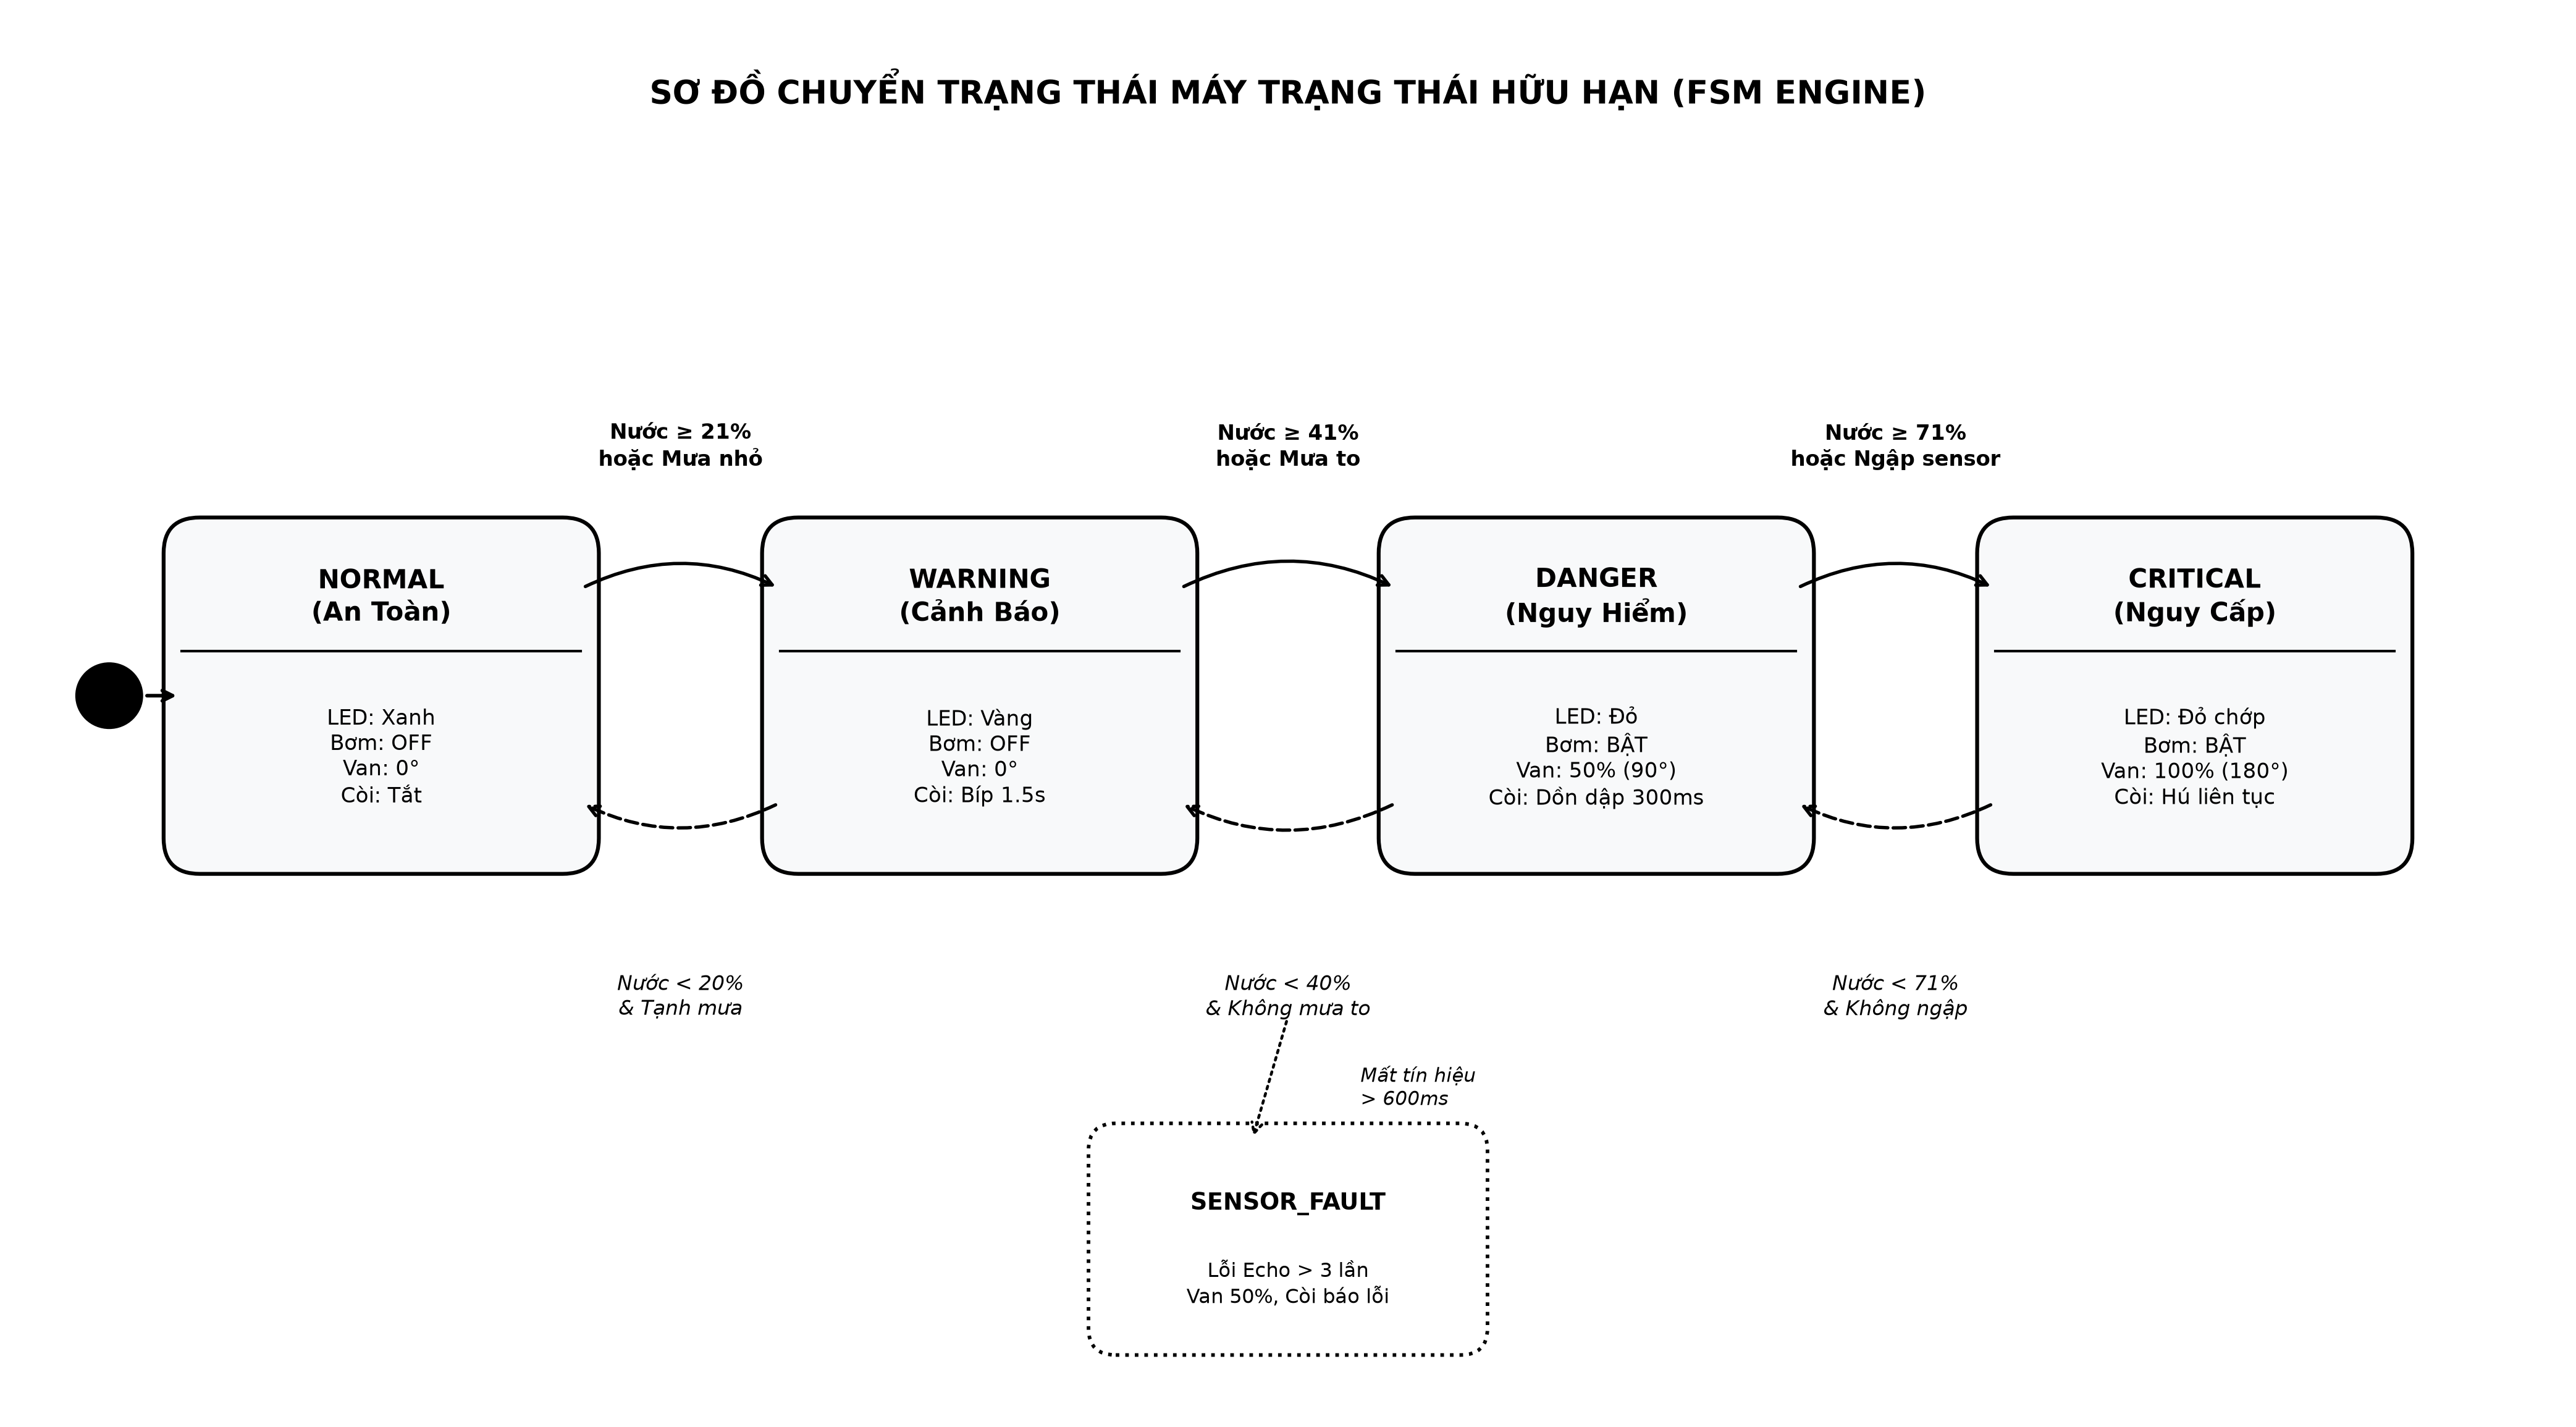
\includegraphics[width=0.95\textwidth]{figures/fsm_state_machine.png}
    \caption{Sơ đồ chuyển trạng thái máy trạng thái hữu hạn FSM của hệ thống FloodGuard}
    \label{fig:fsm_diagram}
\end{figure}

\subsection{Bảng Ma Trận Chuyển Trạng Thái (State Transition~Table)}
Ma trận chuyển dịch giữa các trạng thái được xác định chặt chẽ dựa trên các biểu thức điều kiện bảo vệ (\textit{Guard Conditions}) kết hợp thông số mực nước và lượng mưa (Bảng~\ref{tab:fsm_transitions}).

\begingroup
\setlength{\tabcolsep}{4.5pt}
\small
\renewcommand{\arraystretch}{1.25}
\begin{longtable}{|>{\raggedright\arraybackslash}p{2.8cm}|>{\raggedright\arraybackslash}p{4.35cm}|>{\raggedright\arraybackslash}p{2.9cm}|>{\raggedright\arraybackslash}p{4.45cm}|}
\caption{Bảng ma trận chuyển trạng thái của thuật toán FSM kết hợp dải trễ Hysteresis} \label{tab:fsm_transitions} \\
\hline
\textbf{Trạng thái hiện tại} & \textbf{Điều kiện kích hoạt chuyển dịch (Guards)} & \textbf{Trạng thái kế tiếp} & \textbf{Hành động thực thi khi vào trạng thái} \\ \hline
\endfirsthead

\multicolumn{4}{c}%
{{\bfseries Bảng \thetable{} -- Tiếp theo từ trang trước}} \\
\hline
\textbf{Trạng thái hiện tại} & \textbf{Điều kiện kích hoạt chuyển dịch (Guards)} & \textbf{Trạng thái kế tiếp} & \textbf{Hành động thực thi khi vào trạng thái} \\ \hline
\endhead

\hline \multicolumn{4}{|r|}{{\footnotesize\textit{(Còn tiếp ở trang sau)}}} \\ \hline
\endfoot

\hline
\endlastfoot

\texttt{STATE\_NORMAL} & $P_{\text{water}} \ge 71\%$ hoặc \texttt{isSubmerged} & \texttt{STATE\_CRITICAL} & Bật bơm, mở van $100\%$, LED đỏ chớp, còi hú liên tục. \\
 & $P_{\text{water}} \ge 41\%$ hoặc \texttt{isHeavyRain} & \texttt{STATE\_DANGER} & Bật bơm (nếu $P \ge 20\%$), mở van $50\%$, LED đỏ sáng, còi dồn dập $400\,\text{ms}$. \\
 & $P_{\text{water}} \ge 21\%$ hoặc \texttt{isLightRain} & \texttt{STATE\_WARNING} & Tắt bơm, đóng van $0^\circ$, LED vàng sáng, còi bíp thưa $1.5\,\text{s}$. \\ \hline
\texttt{STATE\_WARNING} & $P_{\text{water}} \ge 71\%$ hoặc \texttt{isSubmerged} & \texttt{STATE\_CRITICAL} & Bật bơm, mở van $100\%$, còi hú liên tục. \\
 & $P_{\text{water}} \ge 41\%$ hoặc \texttt{isHeavyRain} & \texttt{STATE\_DANGER} & Bật bơm, mở van $50\%$, còi dồn dập $400\,\text{ms}$. \\
 & $P_{\text{water}} < 18\%$ và tạnh mưa hoàn toàn & \texttt{STATE\_NORMAL} & Tắt còi, LED xanh sáng (an toàn). \\ \hline
\texttt{STATE\_DANGER} & $P_{\text{water}} \ge 71\%$ hoặc \texttt{isSubmerged} & \texttt{STATE\_CRITICAL} & Tăng góc van lên $100\%$, chuyển còi sang hú liên tục. \\
 & $P_{\text{water}} < 38\%$ và không mưa to & \texttt{STATE\_WARNING} & Ngắt bơm (sau $T_{\text{min\_run}} \ge 5\,\text{s}$), đóng van về $0^\circ$, hạ còi. \\ \hline
\texttt{STATE\_CRITICAL} & $P_{\text{water}} < 68\%$ và không ngập sensor & \texttt{STATE\_DANGER} & Giảm van về $50\%$, chuyển còi về nhịp dồn dập $400\,\text{ms}$. \\ \hline
\textbf{Mọi trạng thái} & Mất xung Echo liên tiếp $> 450\,\text{ms}$ (3 chu kỳ) & \texttt{SENSOR\_FAULT} & Tắt bơm (chống cháy bơm), mở van $50\%$ xả an toàn, 3 LED chớp, còi ngắt quãng báo sự cố. \\ \hline
\texttt{SENSOR\_FAULT} & Nhận lại $\ge 5$ mẫu đo ToF hợp lệ liên tiếp & \texttt{STATE\_NORMAL} hoặc cấp tương ứng & Phục hồi vận hành tự động bình thường. \\ \hline
\end{longtable}
\endgroup

\subsection{Bảng Tín Hiệu Đầu Ra Chi Tiết Theo Từng Trạng Thái}
Tương ứng với mỗi trạng thái FSM, hệ thống thiết lập đồng bộ tín hiệu điều khiển trên toàn bộ cơ cấu chấp hành và thiết bị chỉ thị (Bảng~\ref{tab:fsm_outputs}).

\begin{table}[H]
\centering
\caption{Bảng tín hiệu điều khiển đầu ra theo từng trạng thái FSM}
\label{tab:fsm_outputs}
\small
\renewcommand{\arraystretch}{1.2}
\begin{tabularx}{\textwidth}{|p{2.9cm}|>{\centering\arraybackslash}p{1.1cm}|>{\centering\arraybackslash}p{1.1cm}|>{\centering\arraybackslash}p{1.1cm}|X|>{\centering\arraybackslash}p{2.0cm}|>{\centering\arraybackslash}p{2.0cm}|}
\hline
\textbf{Trạng thái FSM} & \textbf{LED Xanh} & \textbf{LED Vàng} & \textbf{LED Đỏ} & \textbf{Còi Buzzer 5V} & \textbf{Relay Bơm} & \textbf{Van Servo} \\ \hline
\texttt{STATE\_NORMAL} & BẬT & TẮT & TẮT & Tắt hoàn toàn (0V) & OFF (High-Z) & Đóng $0^\circ$ ($0\%$) \\ \hline
\texttt{STATE\_WARNING} & TẮT & BẬT & TẮT & Bíp thưa ($120\,\text{ms}$ on / $1380\,\text{ms}$ off) & OFF (High-Z) & Đóng $0^\circ$ ($0\%$) \\ \hline
\texttt{STATE\_DANGER} & TẮT & TẮT & BẬT & Dồn dập ($150\,\text{ms}$ on / $250\,\text{ms}$ off) & ON (Active LOW) & Mở $90^\circ$ ($50\%$) \\ \hline
\texttt{STATE\_CRITICAL} & TẮT & TẮT & Chớp $100\,\text{ms}$ & Hú liên tục ($\approx 2.3\,\text{kHz}$) & ON (Active LOW) & Mở $180^\circ$ ($100\%$) \\ \hline
\texttt{SENSOR\_FAULT} & Chớp & Chớp & Chớp & Bíp ngắt quãng báo sự cố & TẮT (Bảo vệ) & Mở an toàn $90^\circ$ ($50\%$) \\ \hline
\end{tabularx}
\end{table}

\subsection{Mã C++ Hiện Thực FSM Bằng Cấu Trúc Switch-Case}
Đoạn mã C++ chuẩn hóa hiện thực hóa logic FSM, tích hợp dải trễ Hysteresis, bộ lọc Debounce và cơ chế Safety Override:
\begin{lstlisting}[language=C++]
// Bang hang so nguong Hysteresis dong bo toan he thong
const int THRESHOLD_WARN_ENTER   = 21, THRESHOLD_WARN_EXIT   = 18; // Delta = 3%
const int THRESHOLD_DANGER_ENTER = 41, THRESHOLD_DANGER_EXIT = 38; // Delta = 3%
const int THRESHOLD_CRIT_ENTER   = 71, THRESHOLD_CRIT_EXIT   = 68; // Delta = 3%

void evaluateSystemStateAuto() {
  bool isLightRain = isRaining;
  bool isHeavyRain = (rainRawADC < RAIN_ADC_HEAVY);
  bool isSubmerged = (rainRawADC < RAIN_ADC_SUBMERGED);

  // 1. Luon cap nhat FSM va LED/Coi de bao ve an toan ngay ca o MANUAL
  switch (sysState) {
    case STATE_NORMAL:
      if (waterPercent >= THRESHOLD_CRIT_ENTER || isSubmerged) sysState = STATE_CRITICAL;
      else if (waterPercent >= THRESHOLD_DANGER_ENTER || isHeavyRain) sysState = STATE_DANGER;
      else if (waterPercent >= THRESHOLD_WARN_ENTER || isLightRain) sysState = STATE_WARNING;
      break;

    case STATE_WARNING:
      if (waterPercent >= THRESHOLD_CRIT_ENTER || isSubmerged) sysState = STATE_CRITICAL;
      else if (waterPercent >= THRESHOLD_DANGER_ENTER || isHeavyRain) sysState = STATE_DANGER;
      else if (waterPercent < THRESHOLD_WARN_EXIT && !isLightRain) sysState = STATE_NORMAL;
      break;

    case STATE_DANGER:
      if (waterPercent >= THRESHOLD_CRIT_ENTER || isSubmerged) sysState = STATE_CRITICAL;
      else if (waterPercent < THRESHOLD_DANGER_EXIT && !isHeavyRain) sysState = STATE_WARNING;
      break;

    case STATE_CRITICAL:
      if (waterPercent < THRESHOLD_CRIT_EXIT && !isSubmerged) sysState = STATE_DANGER;
      break;
  }

  // 2. Dieu khien co cau chap hanh tu dong (chi khi isAutoMode == true)
  if (isAutoMode) {
    switch (sysState) {
      case STATE_NORMAL:
      case STATE_WARNING:
        pumpState = false; valvePercent = 0; break;
      case STATE_DANGER:
        pumpState = (waterPercent >= 20); // Khoa chong chay kho bom khi nuoc < 20%
        valvePercent = 50; break;
      case STATE_CRITICAL:
        pumpState = true; valvePercent = 100; break;
    }
  } else {
    // MANUAL MODE: Giam sat ghi de an toan toi cao (Safety Override)
    static unsigned long critStart = 0;
    if (sysState == STATE_CRITICAL) {
      if (critStart == 0) critStart = millis();
      else if (millis() - critStart >= 10000) { // Qua 10s o muc CRITICAL
        isAutoMode = true; pumpState = true; valvePercent = 100; // Cuong che cuu ho
        critStart = 0;
      }
    } else critStart = 0;
  }
}
\end{lstlisting}

\section{Nguyên Lý Dải Trễ (Hysteresis) \& Chống Rung Thời Gian}
\label{sec:hysteresis_analysis}

\subsection{Phân Tích Cải Tiến Độ Rộng Dải Trễ (Hysteresis Bandwidth)}
Trong các phiên bản thiết kế đơn giản, khoảng cách dải trễ giữa ngưỡng bật và ngưỡng tắt thường chỉ được đặt chênh lệch $1\%$ (ví dụ bật bơm khi $\ge 41\%$ và tắt khi $< 40\%$). Khoảng cách $1\%$ này tương ứng với độ biến thiên khoảng cách vật lý:
\begin{equation}
\Delta d_{\text{band}} = 1\% \times 45.0\,\text{cm} = 0.45\,\text{cm} = 4.5\,\text{mm}
\end{equation}
Khoảng cách $4.5\,\text{mm}$ này nhỏ hơn biên độ sóng vỗ tự nhiên trên mặt hồ thu khi máy bơm công suất lớn vận hành ($\pm 10 - 20\,\text{mm}$) và ngang bằng với sai số đo lường của cảm biến. Hậu quả là máy bơm vẫn bị bật/tắt liên tục (chattering) khi mặt nước dâng mấp mé ngưỡng $40\%$.

Để khắc phục triệt để, hệ thống áp dụng dải trễ Hysteresis biên độ $3\%$ chuẩn hóa trên toàn bộ các ngưỡng:
\begin{itemize}
    \item \textbf{Cặp ngưỡng NORMAL / WARNING:} Ngưỡng lên là $21\%$ ($d \le 40.55\,\text{cm}$); ngưỡng rút hạ trạng thái là $18\%$ ($d > 41.90\,\text{cm}$) $\to$ Dải trễ $\Delta = 3\% = 1.35\,\text{cm}$.
    \item \textbf{Cặp ngưỡng WARNING / DANGER:} Ngưỡng lên là $41\%$ ($d \le 31.55\,\text{cm}$); ngưỡng rút hạ trạng thái là $38\%$ ($d > 32.90\,\text{cm}$) $\to$ Dải trễ $\Delta = 3\% = 1.35\,\text{cm}$.
    \item \textbf{Cặp ngưỡng DANGER / CRITICAL:} Ngưỡng lên là $71\%$ ($d \le 18.05\,\text{cm}$); ngưỡng rút hạ trạng thái là $68\%$ ($d > 19.40\,\text{cm}$) $\to$ Dải trễ $\Delta = 3\% = 1.35\,\text{cm}$.
\end{itemize}

\noindent\textbf{Đặc thù khi triển khai trên mô hình sa bàn Mica thu nhỏ ($10\,\text{cm}$ nước):}\\
Trên mô hình sa bàn thực tế, dải trễ $3\%$ tương ứng với khoảng dịch chuyển mực nước vật lý chỉ đạt $\Delta d_{\text{mica}} = 3\% \times 10.0\,\text{cm} = 3.0\,\text{mm}$. Khoảng cách $3.0\,\text{mm}$ này tiệm cận với độ phân giải giới hạn của cảm biến siêu âm HC-SR04 và hoàn toàn có thể bị vượt qua bởi các đợt sóng dập dềnh cơ học khi máy bơm mini xả nước. Do đó, nếu chỉ dựa thuần túy vào dải trễ biên độ $3\%$, rơ-le vẫn có nguy cơ bị đóng ngắt dao động. 

Để giải quyết triệt để vấn đề này trên phần cứng thực tế, chốt chặn bảo vệ quyết định của hệ thống chính là sự kết hợp chặt chẽ giữa dải trễ biên độ với **bộ lọc chống rung thời gian Debounce $1.0\,\text{s}$** và **thời gian chạy tối thiểu của máy bơm $5.0\,\text{s}$ (Min-run Time)** được phân tích dưới đây.

\subsection{Cơ Chế Chống Rung Theo Thời Gian (\textit{Time-Based Debouncing \& Dwell Time})}
Song song với dải trễ biên độ, hệ thống bổ sung hai ràng buộc thời gian nghiêm ngặt:
\begin{enumerate}
    \item \textbf{Bộ lọc chống rung thời gian chuyển trạng thái (\textit{Transition Debouncing}):} Điều kiện chuyển trạng thái phải được duy trì liên tục trong thời gian tối thiểu $t_{\text{debounce}} = 1.0\,\text{s}$ (tương đương 5 chu kỳ lấy mẫu liên tiếp). Nếu mặt nước chỉ vọt lên trong chốc lát do một gợn sóng bất chợt rồi tụt xuống ngay, FSM sẽ bỏ qua và không kích hoạt đổi trạng thái.
    \item \textbf{Thời gian vận hành tối thiểu của máy bơm (\textit{Minimum Run/Dwell Time}):} Khi máy bơm được kích hoạt bật, nó bắt buộc phải chạy tối thiểu $t_{\text{min\_run}} = 5.0\,\text{s}$ trước khi được phép ngắt, ngay cả khi mực nước tụt xuống dưới ngưỡng tắt tức thì. Cơ chế này giúp bảo vệ cuộn hút Relay và giảm thiểu tối đa hiện tượng quá nhiệt động cơ do dòng điện khởi động lặp lại liên tục.
\end{enumerate}

\subsection{Đồ Thị So Sánh Đáp Ứng Khi Có và Không Có Hysteresis}
Hình~\ref{fig:hysteresis_graph} minh họa kết quả mô phỏng đáp ứng của rơ-le máy bơm khi mực nước dao động hình sin quanh biên ngưỡng $40\%$.

\begin{figure}[H]
    \centering
    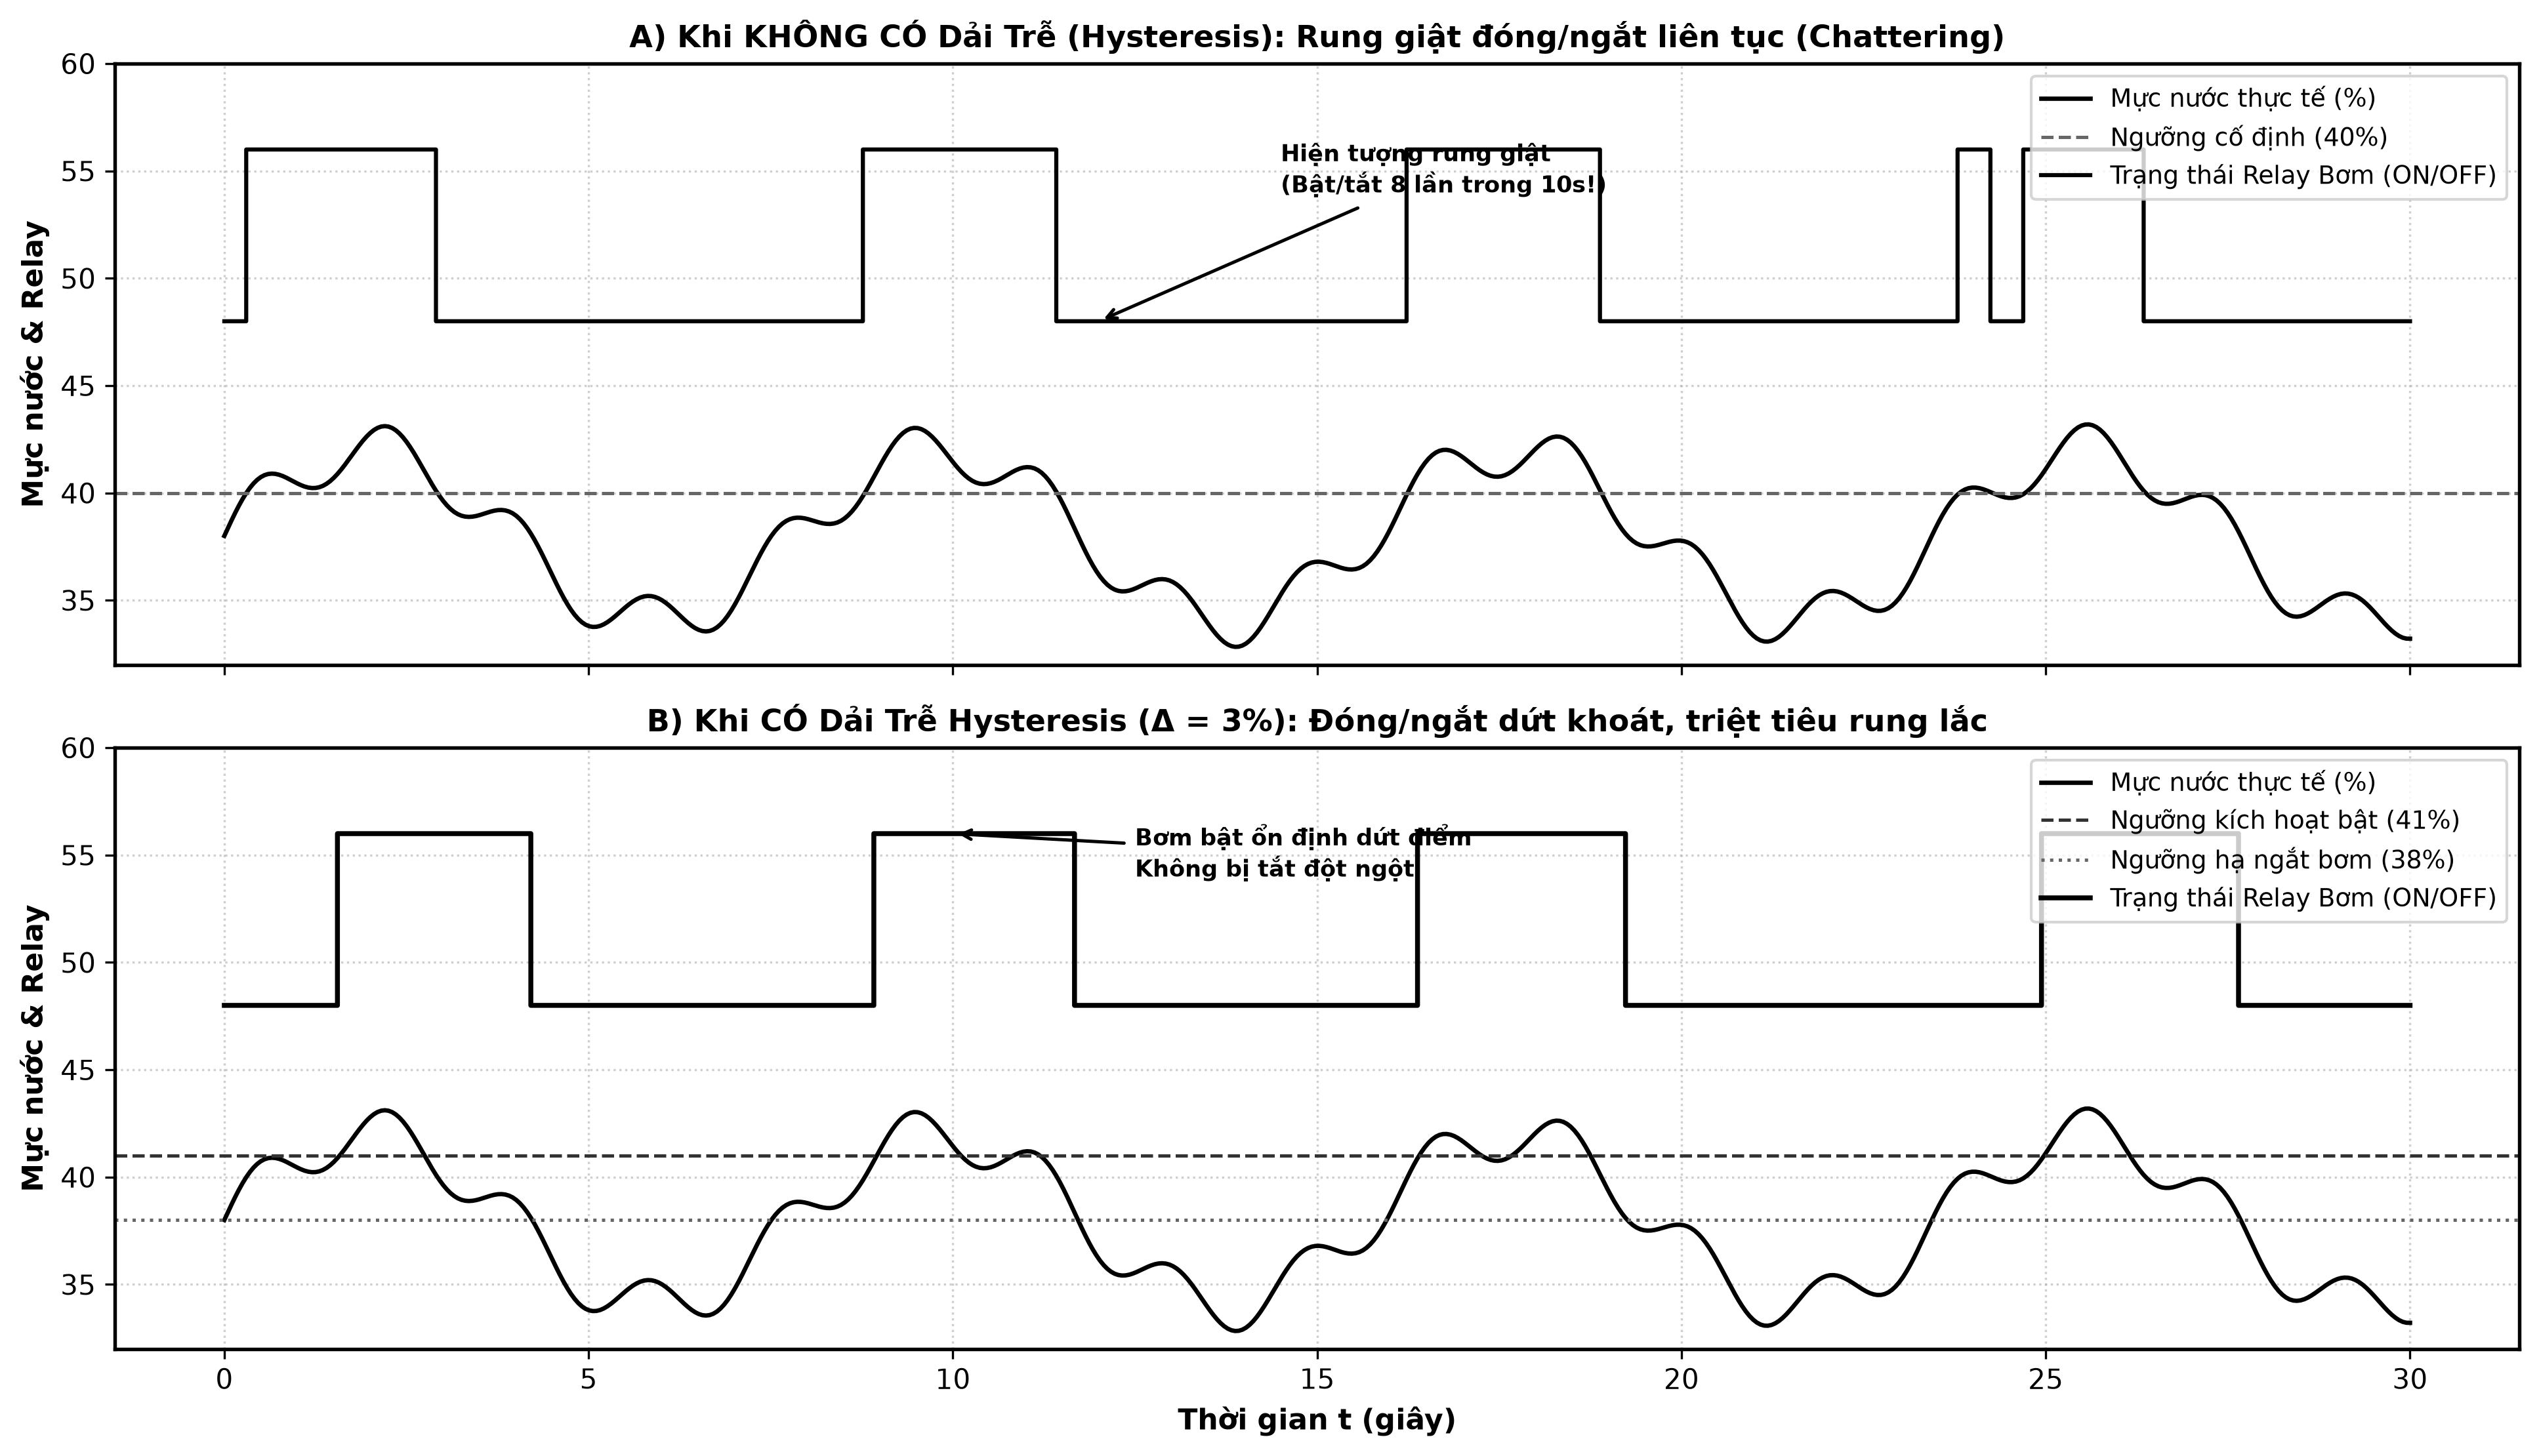
\includegraphics[width=0.95\textwidth]{figures/hysteresis_response.png}
    \caption{So sánh đáp ứng điều khiển máy bơm: Không có Hysteresis (A) và Có Hysteresis (B)}
    \label{fig:hysteresis_graph}
\end{figure}

Ở trường hợp A (không có dải trễ), rơ-le máy bơm bị đóng ngắt tới 8 lần trong vòng 10 giây, gây tổn hại cơ học và nguy cơ cháy tiếp điểm. Ở trường hợp B (áp dụng Hysteresis kết hợp Debouncing), máy bơm chỉ đóng dứt khoát 1 lần khi nước vượt $41\%$ và chỉ ngắt khi nước rút sâu ổn định dưới $38\%$.

\subsection{Thuật Toán Điều Khiển Mượt Servo Van Xả (\textit{Soft PWM Stepping})}
Để tránh hiện tượng động cơ Servo quay giật đột ngột từ $0^\circ$ lên $180^\circ$ trong 1 chu kỳ điều khiển (gây rung lắc gãy khớp nối cơ khí cửa van và tiêu thụ dòng đỉnh lớn gây sụt áp nguồn), hệ thống áp dụng bộ giới hạn tốc độ quay (\textit{Slew-rate Limiter}):
\begin{lstlisting}[language=C++]
// Noi suy goc quay Servo muot ma moi 20ms
if (currentAngle < targetAngle) {
  currentAngle += 5; // Tang moi buoc 5 do
  if (currentAngle > targetAngle) currentAngle = targetAngle;
  valveServo.write(currentAngle);
} else if (currentAngle > targetAngle) {
  currentAngle -= 5; // Giam moi buoc 5 do
  if (currentAngle < targetAngle) currentAngle = targetAngle;
  valveServo.write(currentAngle);
}
\end{lstlisting}
Thuật toán chia hành trình $180^\circ$ thành 36 bước nhỏ cách nhau $20\,\text{ms}$, giúp van xả mở êm ái trong khoảng thời gian $0.72\,\text{s}$.

\section{Chế Độ Vận Hành AUTO / MANUAL \& Bảo Vệ Failsafe}
\label{sec:failsafe_mode}

\subsection{Máy Trạng Thái Quản Lý Chế Độ Vận Hành}
Hệ thống quản lý 3 trạng thái chế độ hoạt động:
\begin{itemize}
    \item \textbf{\texttt{AUTO\_MODE}:} Chế độ mặc định. Quyền điều khiển máy bơm và van xả do thuật toán FSM quyết định tự động $100\%$. Mọi nút can thiệp cưỡng chế trên Web Dashboard đều bị khóa mờ.
    \item \textbf{\texttt{MANUAL\_MODE}:} Chế độ can thiệp thủ công. Người vận hành được phép bật/tắt bơm và xoay góc van xả tùy ý thông qua Web Dashboard để phục vụ kiểm tra thiết bị hoặc xả đáy hồ.
    \item \textbf{\texttt{FAILSAFE\_MODE}:} Trạng thái chuyển đổi khẩn cấp khi hệ thống phát hiện mất kết nối mạng điều khiển từ xa.
\end{itemize}

\subsection{Cơ Chế Heartbeat \& Căn Cứ Chọn Timeout 30 Giây}
\begin{itemize}
    \item \textbf{Định nghĩa Heartbeat:} Trong kiến trúc của FloodGuard, trình duyệt Web Dashboard liên tục gửi yêu cầu \texttt{GET /api/status} mỗi $1000\,\text{ms}$ ($1\,\text{s}$). Mỗi khi nhận được request này, vi điều khiển cập nhật biến dấu thời gian:
    \begin{equation}
        t_{\text{last\_heartbeat}} = \text{millis()}
    \end{equation}
    Yêu cầu polling dữ liệu này vừa làm nhiệm vụ cập nhật giao diện, vừa đóng vai trò như một gói tin điểm danh (\textit{Keep-alive Heartbeat}).
    \item \textbf{Cơ chế kích hoạt Failsafe:} Trong hàm \texttt{loop()}, hệ thống liên tục kiểm tra:
    \begin{equation}
        \Delta t_{\text{offline}} = \text{millis()} - t_{\text{last\_heartbeat}}
    \end{equation}
    Nếu hệ thống đang ở \texttt{MANUAL\_MODE} mà $\Delta t_{\text{offline}} > 30000\,\text{ms}$ ($30\,\text{s}$), vi điều khiển ngay lập tức cưỡng chế thiết lập lại:
    \begin{equation}
        \texttt{isAutoMode = true}
    \end{equation}
    \item \textbf{Lý do lựa chọn ngưỡng $30\,\text{s}$:} 
    Khoảng thời gian $30\,\text{s}$ tương đương với 30 chu kỳ heartbeat bị mất liên tiếp. Con số này đủ dài để bỏ qua các hiện tượng rớt mạng tạm thời do nhiễu sóng Wi-Fi ($2 - 5\,\text{s}$) hoặc khi người dùng vô tình xoay màn hình điện thoại khiến trình duyệt reload, nhưng đủ ngắn để đảm bảo rằng nếu trạm đang bị dâng nước nhanh trong mưa bão, mực nước sẽ không thể dâng vượt quá dung tích hồ thu trước khi hệ thống tự động tiếp quản.
\end{itemize}

\subsection{Hành Vi Khôi Phục Kết Nối \& Quy Tắc Ghi Đè An Toàn Tối Cao}
\begin{itemize}
    \item \textbf{Khôi phục kết nối:} Khi mạng Wi-Fi được kết nối lại và trình duyệt gửi request tiếp theo, ESP32 sẽ trả về chuỗi JSON chứa trường cờ \texttt{"failsafe": true}. Giao diện Web Dashboard sẽ lập tức hiển thị một thanh thông báo màu cam với nội dung: *"Hệ thống đã tự động chuyển về chế độ AUTO do mất kết nối quá 30 giây"*. Để tiếp tục can thiệp thủ công, người vận hành bắt buộc phải nhấp nút xác nhận trên Web để chuyển lại sang MANUAL.
    \item \textbf{Quy tắc ghi đè an toàn tối cao (\textit{Safety Priority Override}):} Ngay cả khi đang ở chế độ MANUAL, nếu mực nước đo được đạt mức nguy cấp CRITICAL ($\ge 71\%$) mà sau $10\,\text{s}$ người vận hành không ra lệnh bật bơm hoặc mở van, hệ thống sẽ tự động tước quyền MANUAL, chuyển về AUTO và kích hoạt toàn bộ cơ cấu xả lũ hết công suất để chống tràn hồ.

\end{itemize}

\section{Phân Tích Đặc Tính Thời Gian Thực (Real-Time Performance Analysis)}

\subsection{Chu Kỳ Vòng Lặp Thực Tế \& Đánh Giá Độ Trễ}
Thời gian thực thi một chu kỳ vòng lặp \texttt{loop()} được đo đạc thực tế bằng hàm \texttt{micros()} trên vi điều khiển ESP32:
\begin{itemize}
    \item \textbf{Khi không có kết nối Web (Chu kỳ nền):} Thời gian chạy một vòng lặp chỉ mất $2 - 5\,\text{ms}$, phần lớn thời gian CPU ở trạng thái rảnh hoặc thực thi băm xung nhịp còi.
    \item \textbf{Tại chu kỳ trích mẫu cảm biến (mỗi $150\,\text{ms}$):} Mất khoảng $36 - 38\,\text{ms}$ (chủ yếu là thời gian đo xung ToF của cảm biến siêu âm qua hàm \texttt{pulseIn()}).
    \item \textbf{Khi xử lý yêu cầu HTTP JSON:} Mất khoảng $8 - 15\,\text{ms}$ để đọc thông số, định dạng chuỗi JSON và gửi qua ngăn xếp TCP/IP.
\end{itemize}

\subsection{Thời Gian Phản Ứng Tối Đa (Worst-Case Reaction Time - WCRT)}
\label{sec:wcrt_analysis}
Thời gian phản ứng tồi tệ nhất trong tình huống khẩn cấp ($T_{\text{WCRT\_urgent}}$) được tính từ thời điểm mực nước thực tế chạm ngưỡng nguy hiểm hoặc ngập tràn khẩn cấp cho tới khi tiếp điểm Relay đóng hoàn toàn để cấp điện cho máy bơm (không qua bộ lọc thời gian debounce hoặc khi debounce đã tích lũy đủ):
\begin{equation}
T_{\text{WCRT\_urgent}} = T_{\text{sample\_wait}} + T_{\text{filter\_typical}} + T_{\text{FSM}} + T_{\text{relay\_delay}}
\end{equation}
Trong đó:
\begin{itemize}
    \item $T_{\text{sample\_wait}} = 150\,\text{ms}$: Thời gian chờ tối đa giữa hai chu kỳ kích hoạt đọc cảm biến.
    \item $T_{\text{filter\_typical}} = 36\,\text{ms}$: Thời gian đo 3 mẫu siêu âm của bộ lọc trung vị trong điều kiện bình thường ($3 \times 12\,\text{ms}$).
    \item $T_{\text{FSM}} = 2\,\text{ms}$: Thời gian tính toán thuật toán FSM và cập nhật chân GPIO.
    \item $T_{\text{relay\_delay}} = 15\,\text{ms}$: Thời gian trễ cơ học để tiếp điểm lá đồng của Relay 5V đóng kín hoàn toàn mạch điện.
\end{itemize}
Tổng thời gian phản ứng khẩn cấp:
\begin{equation}
T_{\text{WCRT\_urgent}} = 150 + 36 + 2 + 15 = 203\,\text{ms} < 250\,\text{ms}
\end{equation}
Kết quả chứng minh hệ thống đáp ứng xuất sắc ràng buộc thời gian thực $\le 250\,\text{ms}$ đối với các tình huống phản ứng khẩn cấp, đảm bảo máy bơm được kích hoạt gần như tức thời khi nước vừa chạm ngưỡng tràn.

\noindent\textbf{Thời gian đáp ứng ổn định có lọc chống rung (\textit{Debounced Stable Transition}):}\\
Đối với quá trình chuyển trạng thái FSM thông thường giữa các cấp độ nhằm tránh rung tiếp điểm rơ-le do sóng vỗ dao động, điều kiện chuyển trạng thái cần được duy trì ổn định liên tục qua bộ lọc thời gian $t_{\text{debounce}} = 1.0\,\text{s}$. Do đó, thời gian đáp ứng tổng thể của hệ thống khi xác lập trạng thái chuyển cấp FSM bền vững là:
\begin{equation}
T_{\text{stable}} = T_{\text{WCRT\_urgent}} + t_{\text{debounce}} \approx 203\,\text{ms} + 1000\,\text{ms} \approx 1.203\,\text{s}
\end{equation}
Việc phân định rõ hai mốc thời gian này giúp hệ thống vừa bảo đảm an toàn cơ học cho rơ-le trong vận hành thông thường, vừa bảo đảm thời gian phát hiện và xử lý khẩn cấp dưới $250\,\text{ms}$.

\noindent\textbf{Phân tích độ trễ chặn luồng tối đa khi mất tín hiệu siêu âm:}\\
Cần lưu ý rằng hàm \texttt{pulseIn()} trong ESP32 Arduino Core là hàm chặn CPU (\textit{blocking}). Trong kịch bản xấu nhất khi cảm biến siêu âm bị mất xung Echo hoàn toàn, mỗi lượt đo sẽ phải chờ hết thời gian timeout $30\,\text{ms}$. Với bộ lọc 3 mẫu, CPU sẽ bị chặn tối đa $T_{\text{filter\_worst}} = 3 \times 30\,\text{ms} = 90\,\text{ms}$. Ngay cả trong kịch bản tồi tệ này, tổng thời gian chu kỳ quét vẫn nằm trong mức $150 + 90 + 2 = 242\,\text{ms} < 250\,\text{ms}$ trước khi rơi vào cơ chế bảo vệ giữ mẫu.

\subsection{Cơ Chế Phục Vụ Yêu Cầu Mạng Wi-Fi / HTTP}
Thư viện \texttt{WebServer.h} của ESP32 Arduino Core hoạt động theo kiến trúc đồng bộ tuần tự (\textit{synchronous polling}) trên cùng luồng chính \texttt{loopTask}. Trong hàm \texttt{loop()}, lời gọi \texttt{server.handleClient()} thực hiện kiểm tra và xử lý các kết nối socket TCP đang chờ từ lớp mạng lwIP. Trong điều kiện bình thường khi không có yêu cầu mới, hàm trả về quyền điều khiển rất nhanh ($< 0.1\,\text{ms}$), không ảnh hưởng đến chu kỳ đo lường.

Tuy nhiên, do hoạt động đồng bộ, nếu máy khách truyền dữ liệu chập chờn (\textit{slow client}) hoặc gửi yêu cầu vào đúng thời điểm vi điều khiển đang xử lý, thời gian chiếm dụng CPU có thể kéo dài $10 - 30\,\text{ms}$. Để triệt tiêu tối đa hiện tượng trễ vòng lặp này:
\begin{itemize}
    \item Toàn bộ dữ liệu phản hồi API JSON được thu gọn tối đa ($\approx 210$ byte), truyền trực tiếp trong một khung mạng TCP duy nhất.
    \item Trang Web Dashboard tĩnh được lưu trong bộ nhớ Flash và truyền phát bằng phương thức \texttt{server.send\_P()}, tránh hoàn toàn việc cấp phát bộ nhớ động RAM (heap) và giảm thiểu số vòng lặp chờ xử lý.
\end{itemize}

\subsection{Bảo Vệ Hệ Thống Bằng Phần Cứng Task Watchdog Timer (TWDT)}
Khác với cơ chế bảo vệ Failsafe $30\,\text{s}$ ở tầng ứng dụng mạng Web (Mục~\ref{sec:failsafe_mode}), để phòng ngừa tình huống vi điều khiển bị treo CPU do sốc điện, xung nhiễu nguồn hoặc bẫy lặp phần mềm vô hạn, FloodGuard tích hợp trực tiếp bộ giám sát Task Watchdog Timer (TWDT) của hệ điều hành thời gian thực ESP-IDF FreeRTOS.

Bộ giám sát TWDT được gắn vào tác vụ chính \texttt{loopTask} thông qua API \texttt{esp\_task\_wdt\_add(NULL)} với chu kỳ timeout được cấu hình là $3000\,\text{ms}$ ($3\,\text{s}$). Lệnh xóa cờ \texttt{esp\_task\_wdt\_reset()} được gọi đều đặn ở đầu mỗi chu kỳ \texttt{loop()}. Nếu sau $3\,\text{s}$ vòng lặp không thể quay lại điểm xóa cờ (ví dụ do hàm \texttt{pulseIn()} bị treo phần cứng hoặc hàm Web bị nghẽn socket), ngắt phần cứng TWDT sẽ ngay lập tức được kích hoạt, ghi lại nhật ký lỗi (core dump) và thực hiện Reset phần cứng tự động để đưa toàn bộ trạm về trạng thái an toàn ban đầu.

\section{Xử Lý Sự Cố \& Ma Trận An Toàn (Fault Handling Matrix)}

Bảng~\ref{tab:fault_matrix} tổng hợp toàn bộ các kịch bản lỗi phần cứng và phần mềm, cùng các phản ứng xử lý an toàn tương ứng được cài đặt sẵn trong firmware.

\begin{table}[H]
\centering
\caption{Ma trận xử lý sự cố và trạng thái an toàn của trạm FloodGuard}
\label{tab:fault_matrix}
\small
\renewcommand{\arraystretch}{1.3}
\begin{tabularx}{\textwidth}{|p{3.2cm}|p{3.8cm}|X|}
\hline
\textbf{Tình huống sự cố} & \textbf{Cơ chế phát hiện} & \textbf{Hành vi ứng phó an toàn của hệ thống} \\ \hline
\textbf{HC-SR04 mất xung Echo} (đứt dây, bám bẩn màng loa) & \texttt{pulseIn()} trả về $0$ hoặc quá timeout $30\,\text{ms}$. & Giữ mẫu hợp lệ gần nhất trong 3 chu kỳ ($450\,\text{ms}$). Nếu lỗi kéo dài $\ge 3$ chu kỳ: chuyển sang \texttt{SENSOR\_FAULT}, còi bíp cảnh báo lỗi, ngắt máy bơm tránh chạy cạn, mở van xả $50\%$ phòng ngừa ngập úng. Tự động phục hồi về FSM bình thường khi có $\ge 5$ mẫu siêu âm hợp lệ liên tiếp. \\ \hline
\textbf{Mực nước dâng vượt miệng cảm biến} ($d < d_{\text{full}}$) & Cảm biến đo khoảng cách $< 5.0\,\text{cm}$. & Đây là tình huống ngập tràn khẩn cấp (\textit{water surge}), hệ thống lập tức cưỡng chế FSM lên trạng thái \texttt{CRITICAL}, bật bơm hết công suất và mở van xả $100\%$ để thoát lũ, không xem là lỗi cảm biến. \\ \hline
\textbf{Khoảng cách ngoài dải đáy bể} ($d > d_{\text{empty}}$) & Cảm biến đo khoảng cách $> 50.0\,\text{cm}$. & Bể cạn hoàn toàn hoặc đáy sâu bất thường; hệ thống tự động kẹp (\textit{clamp}) giá trị về $0\%$, ngắt bơm ngay lập tức để chống chạy khô. \\ \hline
\textbf{Cảm biến mưa hở mạch / đứt dây tín hiệu AO} & Chân GPIO35 (Input-only, không pull-up nội) bị thả nổi. & Nếu thả nổi, ADC có thể đọc ngẫu nhiên về mức thấp kích hoạt nhầm \texttt{isSubmerged}. Thiết kế phần cứng bắt buộc gắn trở kéo ngoài $100\,\text{k}\Omega$ lên $3.3\,\text{V}$ để khi đứt dây, ADC luôn đọc $4095$ (khô ráo), hệ thống tự hành an toàn dựa vào mực nước siêu âm. \\ \hline
\textbf{Mất kết nối Wi-Fi / Đứt mạng Web Client} & Không nhận được gói tin heartbeat quá $30\,\text{s}$. & Tự động hủy chế độ MANUAL, cưỡng chế chuyển về AUTO, trao quyền cho FSM để tự hành chống tràn bể. \\ \hline
\textbf{Sụt áp nguồn cấp (Brown-out)} & Điện áp vi điều khiển tụt dưới ngưỡng $2.8\,\text{V}$. & Bộ giám sát Brown-out Reset nội của ESP32 tự động ngắt vi điều khiển và khởi động lại an toàn khi nguồn ổn định. \\ \hline
\end{tabularx}
\end{table}

\chapter{Giao Diện Web Dashboard \& Tích Hợp Hệ Thống IoT}
\label{ch:web_dashboard}

\section{Tổng Quan Kiến Trúc Mạng \& Chế Độ Hoạt Động}

\subsection{Cấu Hình Mạng Không Dây Nội Bộ SoftAP}
Trong kiến trúc của trạm chống ngập FloodGuard, vi điều khiển ESP32 được cấu hình hoạt động ở chế độ trạm phát không dây độc lập (\textit{Software Access Point - SoftAP Mode}). Đây là giải pháp tối ưu cho các trạm quan trắc dã chiến ngoài thực địa:
\begin{itemize}
    \item \textbf{Độc lập hoàn toàn với hạ tầng mạng bên ngoài:} Hệ thống tự phát sóng Wi-Fi riêng mà không cần kết nối tới Internet hay phụ thuộc vào các bộ định tuyến Router dân dụng (vốn rất dễ mất điện hoặc đứt cáp quang trong bão lũ).
    \item \textbf{Tên mạng truy cập (SSID):} \texttt{FloodGuard\_AP}.
    \item \textbf{Chuẩn bảo mật \& Mật khẩu:} WPA2-PSK với mật khẩu mặc định \texttt{12345678} (đáp ứng tiêu chuẩn an toàn tối thiểu 8 ký tự).
    \item \textbf{Địa chỉ mạng cục bộ (Local Gateway IP):} Cổng mặc định \texttt{192.168.4.1}, cùng mặt nạ mạng con \texttt{255.255.255.0}.
    \item \textbf{Hỗ trợ dịch vụ tên miền đa hướng (mDNS):} Hệ thống tích hợp giao thức mDNS (\textit{Multicast DNS}) thông qua thư viện \texttt{ESPmDNS.h}. Người vận hành chỉ cần nhập địa chỉ tên miền cục bộ dễ nhớ:
    \begin{equation}
        \text{\url{http://floodguard.local}}
    \end{equation}
    vào thanh địa chỉ trình duyệt thay vì phải ghi nhớ chuỗi số IP tĩnh.
\end{itemize}

\section{Bố Cục Giao Diện Người Dùng Dark Glassmorphism}

Giao diện Web Dashboard được thiết kế theo ngôn ngữ hiện đại \textbf{Dark Glassmorphism} (nền tối kết hợp hiệu ứng kính mờ trong suốt), tối ưu hóa hiển thị tự co giãn (\textit{Responsive Design}) trên cả điện thoại di động và máy tính bảng (Hình~\ref{fig:dashboard_mockup}).

\begin{figure}[H]
    \centering
    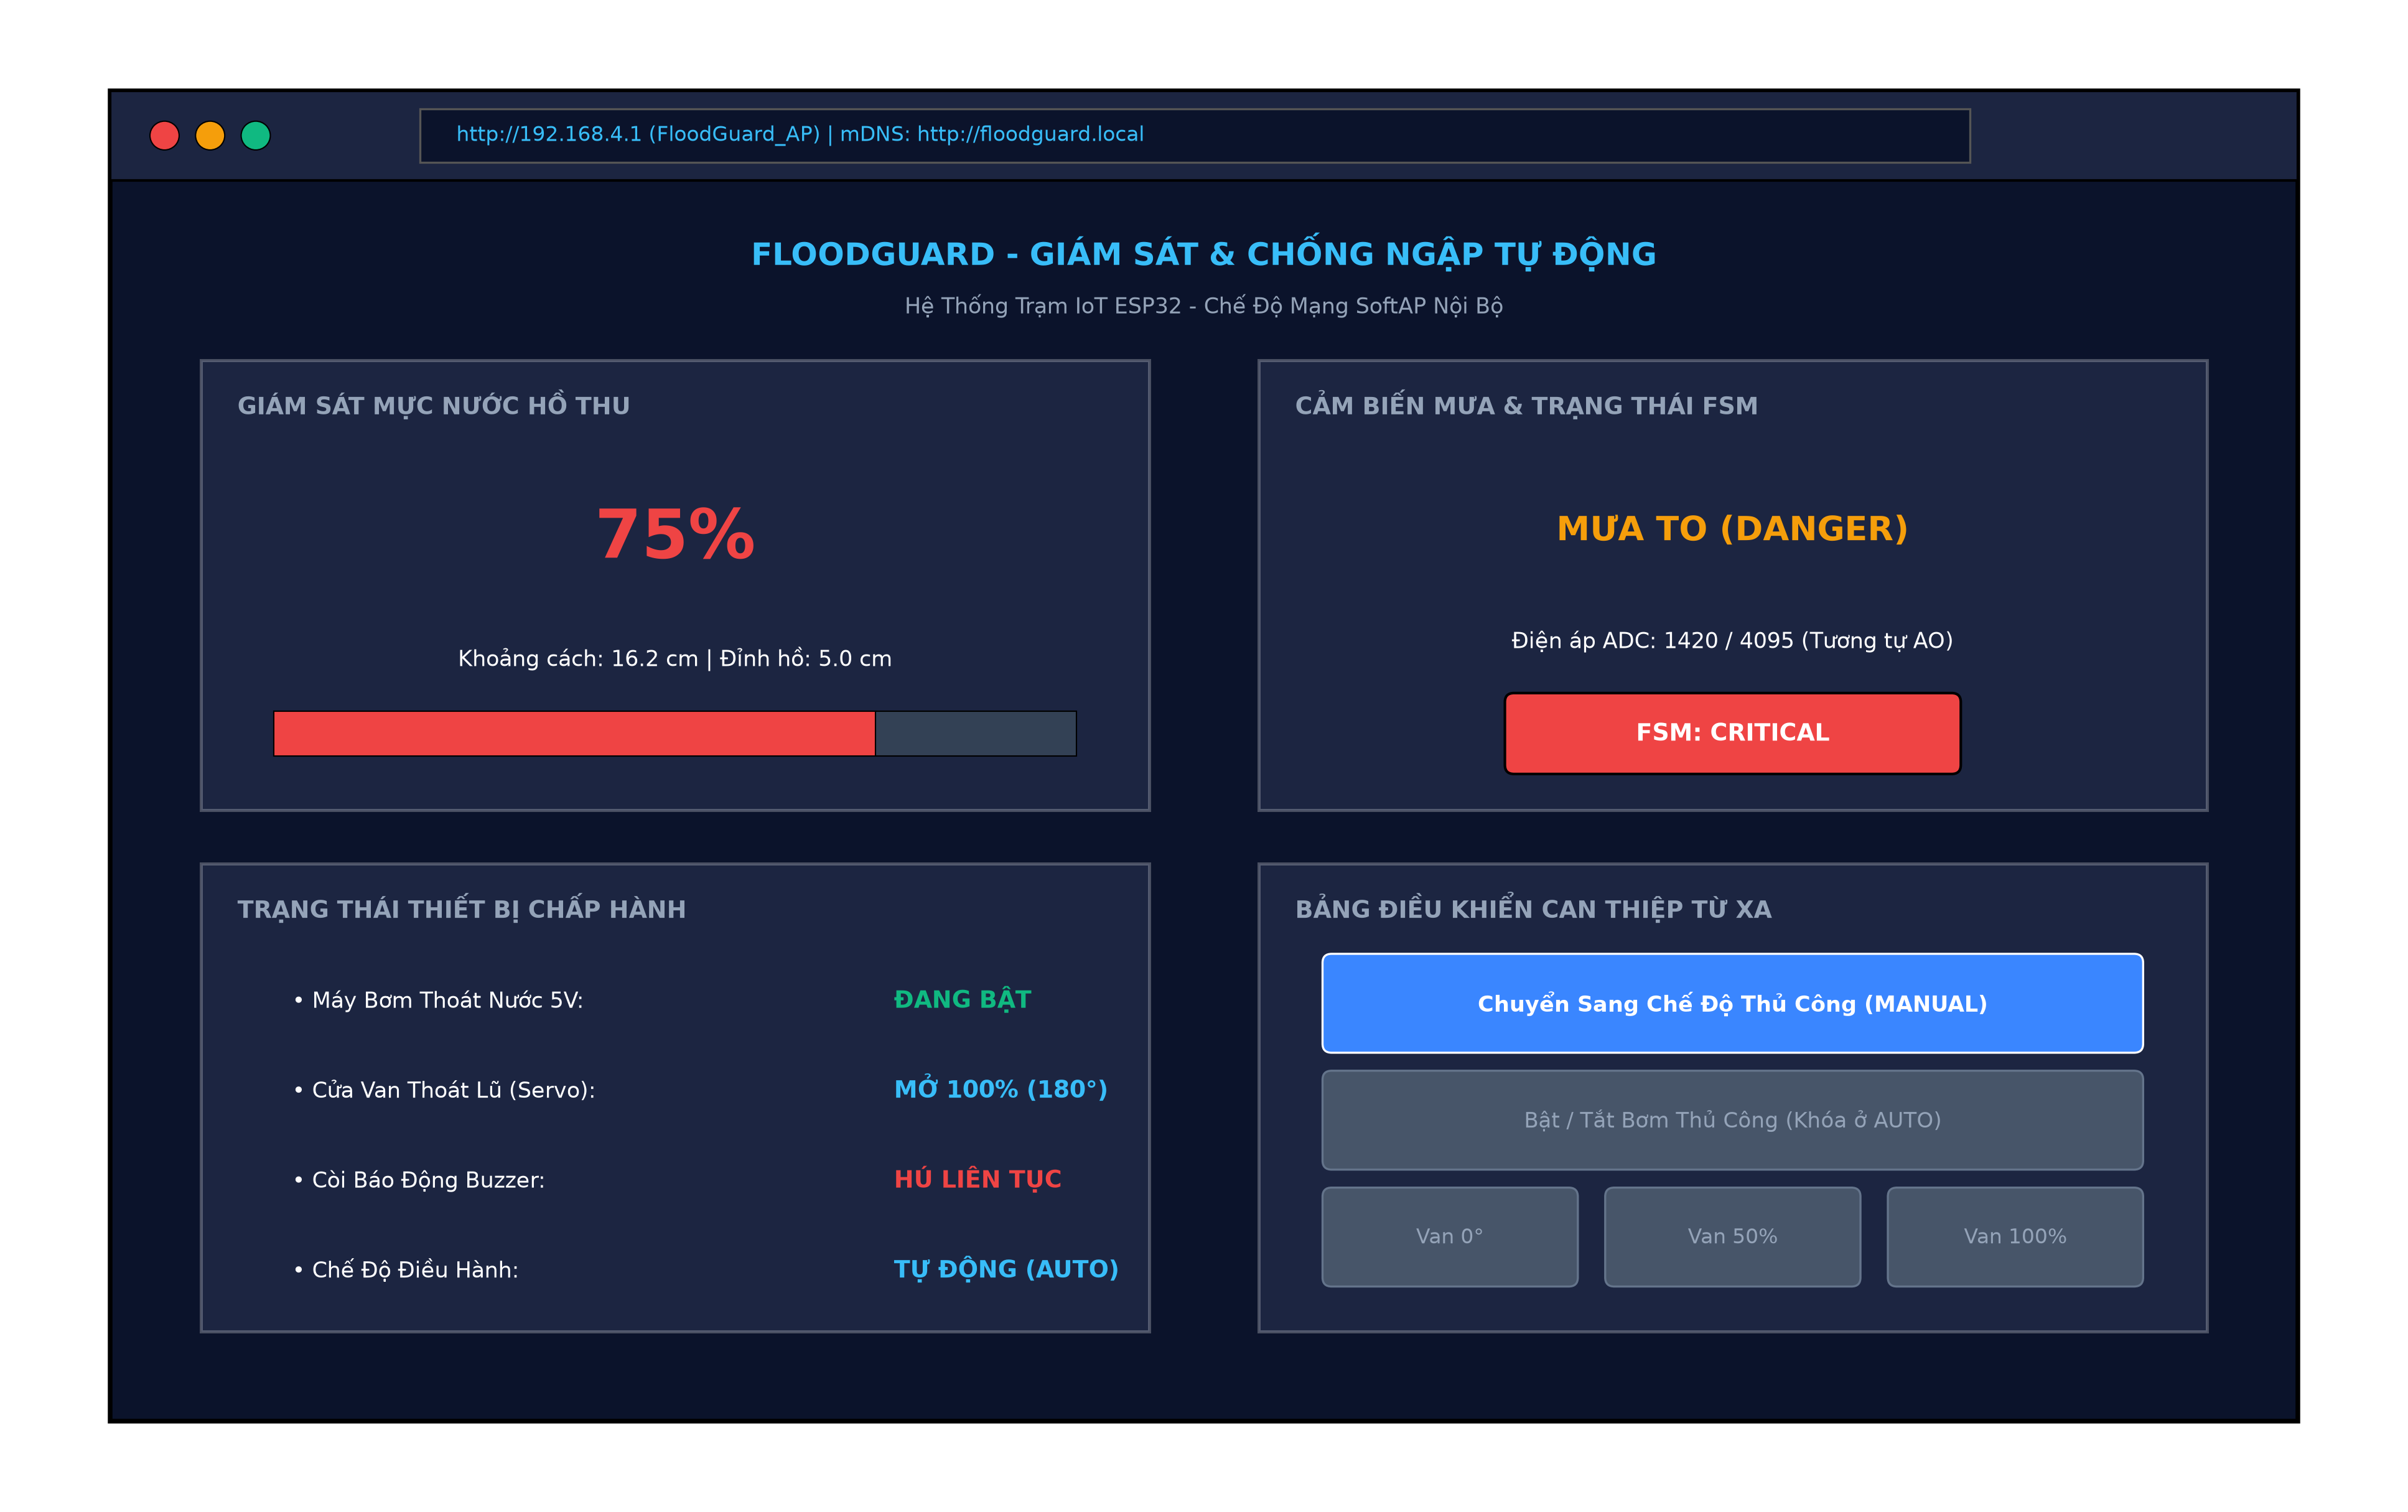
\includegraphics[width=0.98\textwidth]{figures/dashboard_mockup.png}
    \caption{Giao diện Web Dashboard thời gian thực của trạm FloodGuard}
    \label{fig:dashboard_mockup}
\end{figure}

Giao diện trực quan bao gồm 6 khối chức năng chính:
\begin{enumerate}
    \item \textbf{Khối tiêu đề \& Huy hiệu kết nối (Header Badge):} Hiển thị tên trạm, chế độ kết nối mạng SoftAP và địa chỉ IP làm việc hiện thời.
    \item \textbf{Khối giám sát mực nước hồ thu (Water Level Card):} Hiển thị số đo phần trăm dung tích hồ thu cỡ lớn ($0\% - 100\%$), khoảng cách vật lý từ cảm biến tới mặt nước theo đơn vị $\text{cm}$ và thanh tiến trình đồ họa đổi màu tương ứng (Xanh: NORMAL, Vàng: WARNING, Đỏ: DANGER/CRITICAL).
    \item \textbf{Khối cảm biến lượng mưa \& Trạng thái FSM (Rain \& State Card):} Cập nhật phân loại thời tiết theo 4 cấp độ (Khô ráo, Mưa nhỏ, Mưa to, Ngập nước), hiển thị điện áp ADC 12-bit thô và huy hiệu màu sắc phản ánh trạng thái logic FSM hiện hành.
    \item \textbf{Khối giám sát cơ cấu chấp hành (Actuators Status Card):} Hiển thị chi tiết tình trạng đóng/ngắt của máy bơm 5V (ĐANG BẬT / ĐÃ TẮT), góc mở của van xả lũ (Đóng kín $0\%$, Mở vừa $50\%$, Mở tối đa $100\%$) và mức cảnh báo của còi hú.
    \item \textbf{Khối nút bấm chuyển chế độ (Mode Toggle):} Nút bấm chuyển đổi qua lại giữa chế độ vận hành tự động (\texttt{AUTO}) và can thiệp thủ công (\texttt{MANUAL}).
    \item \textbf{Khối nút bấm can thiệp cưỡng chế (Manual Override Controls):} Gồm nút Bật/Tắt máy bơm mini và bộ 3 nút điều chỉnh góc mở cửa van ($0^\circ, 90^\circ, 180^\circ$). Các nút này chỉ được phép kích hoạt khi hệ thống đang ở chế độ MANUAL.
\end{enumerate}

\section{Đặc Tả Chuẩn Hóa Giao Thức HTTP REST API}

Hệ thống giao tiếp hai chiều giữa trình duyệt người dùng và vi điều khiển ESP32 thông qua các endpoint REST API được chuẩn hóa trong Bảng~\ref{tab:api_specifications}.

\begin{table}[H]
\centering
\caption{Bảng đặc tả các giao diện lập trình ứng dụng HTTP REST API của trạm FloodGuard}
\label{tab:api_specifications}
\small
\renewcommand{\arraystretch}{1.3}
\begin{tabularx}{\textwidth}{|l|c|l|c|X|}
\hline
\textbf{Endpoint URL} & \textbf{Method} & \textbf{Tham số truyền} & \textbf{Mã HTTP} & \textbf{Cấu trúc dữ liệu phản hồi \& Chức năng} \\ \hline
\texttt{/} & \texttt{GET} & Không có & 200 & Trả về toàn bộ mã nguồn HTML/CSS/JS của trang Dashboard lưu trong bộ nhớ Flash PROGMEM. \\ \hline
\texttt{/api/status} & \texttt{GET} & Không có & 200 & Trả về chuỗi JSON chứa toàn bộ dữ liệu telemetry đo đạc thời gian thực và trạng thái thiết bị. \\ \hline
\texttt{/api/control} & \texttt{GET} & \texttt{action=mode\_toggle} & 200 & Đảo trạng thái giữa AUTO và MANUAL. \\
 & & \texttt{action=pump\_toggle} & 200 & Bật hoặc ngắt máy bơm cưỡng chế (chỉ ở MANUAL). \\
 & & \texttt{action=valve\_0} & 200 & Xoay Servo đóng kín van $0^\circ$ (chỉ ở MANUAL). \\
 & & \texttt{action=valve\_50} & 200 & Xoay Servo mở van xả $50\%$ ($90^\circ$). \\
 & & \texttt{action=valve\_100} & 200 & Xoay Servo mở van xả tối đa $100\%$ ($180^\circ$). \\ \hline
\end{tabularx}
\end{table}

\subsection{Cấu Trúc Gói Tin JSON Telemetry Chi Tiết}
Tại endpoint \texttt{GET /api/status}, vi điều khiển ESP32 đóng gói các tham số vận hành vào một đối tượng JSON nhỏ gọn:
\begin{lstlisting}[language=C++]
{
  "waterPercent": 75,
  "distance": 16.2,
  "isRaining": true,
  "rainRaw": 1420,
  "rainLevel": "MUA_TO (DANGER)",
  "sysState": "CRITICAL",
  "isAuto": true,
  "pump": true,
  "valve": 100,
  "buzzer": "HU_LIEN_TUC",
  "failsafe": false
}
\end{lstlisting}

\section{Phân Tích Cải Tiến Thiết Kế API \& Hạn Chế Của Phương Thức GET}

\subsection{Phân Tích Rủi Ro Kỹ Thuật Khi Sử Dụng Phương Thức GET Cho Lệnh Điều Khiển}
Trong kiến trúc phần mềm RESTful chuẩn mực quốc tế (RFC 7231):
\begin{itemize}
    \item Phương thức \textbf{\texttt{GET}} được định nghĩa là phương thức an toàn (\textit{Safe}) và có tính bảo lưu trạng thái (\textit{Idempotent}) -- nghĩa là các yêu cầu \texttt{GET} chỉ được dùng để truy vấn dữ liệu mà tuyệt đối không được làm thay đổi trạng thái tài nguyên trên máy chủ.
    \item Việc phiên bản thực nghiệm hiện tại sử dụng request \texttt{GET /api/control} đi kèm tham số hành động (ví dụ \texttt{action=pump\_toggle}) tiềm ẩn các rủi ro bảo mật và vận hành:
    \begin{enumerate}
        \item \textbf{Cơ chế nạp trước liên kết của trình duyệt (\textit{Browser Link Prefetching}):} Một số trình duyệt web hiện đại có tính năng tự động gửi ngầm các request GET đối với các đường dẫn xuất hiện trong trang để tăng tốc độ lướt web. Điều này có thể vô tình kích hoạt bật/tắt máy bơm mà người dùng không hề hay biết.
        \item \textbf{Bộ đệm trình duyệt (\textit{HTTP Caching}):} Trình duyệt hoặc proxy mạng có thể lưu lại kết quả của lệnh GET trước đó và trả về kết quả đệm thay vì gửi lệnh thực sự tới ESP32, dẫn tới sai lệch trạng thái điều khiển.
        \item \textbf{Lịch sử duyệt web (\textit{Browser History \& Bookmarking}):} Người dùng vô tình bookmark hoặc mở lại lịch sử URL có thể gửi lại lệnh bật bơm ngoài ý muốn.
    \end{enumerate}
\end{itemize}

\subsection{Giải Pháp Chuẩn Hóa Kiến Trúc API Cho Phiên Bản Công Nghiệp}
Báo cáo thẳng thắn nhìn nhận đây là một \textbf{hạn chế kỹ thuật trong phiên bản mô hình thử nghiệm ban đầu (Proof of Concept)}. Trong phiên bản hoàn thiện triển khai công nghiệp, hệ thống được quy hoạch nâng cấp toàn diện:
\begin{itemize}
    \item Chuyển đổi toàn bộ các lệnh can thiệp phần cứng sang phương thức \texttt{POST} tại endpoint \texttt{/api/control} với dữ liệu truyền trong thân gói tin (\textit{Request Body}) dưới định dạng JSON:
    \begin{lstlisting}[language=C++]
POST /api/control HTTP/1.1
Content-Type: application/json
Authorization: Bearer <JWT_SECURITY_TOKEN>

{
  "targetDevice": "pump",
  "commandState": "ON",
  "authConfirm": true
}
    \end{lstlisting}
    \item Tích hợp cơ chế mã thông báo chống giả mạo yêu cầu chéo trang (\textit{Anti-CSRF Token}) và kiểm tra quyền quản trị trước khi vi điều khiển thực thi lệnh chuyển mạch GPIO.
\end{itemize}

\section{Sơ Đồ Tuần Tự (Sequence Diagram) Tương Tác Web}

Mối quan hệ tương tác thời gian giữa Người vận hành (trình duyệt Web), máy chủ ESP32 Web Server và cơ cấu chấp hành phần cứng được mô hình hóa qua hai luồng nghiệp vụ trong Hình~\ref{fig:sequence_diagram}.

\begin{figure}[H]
    \centering
    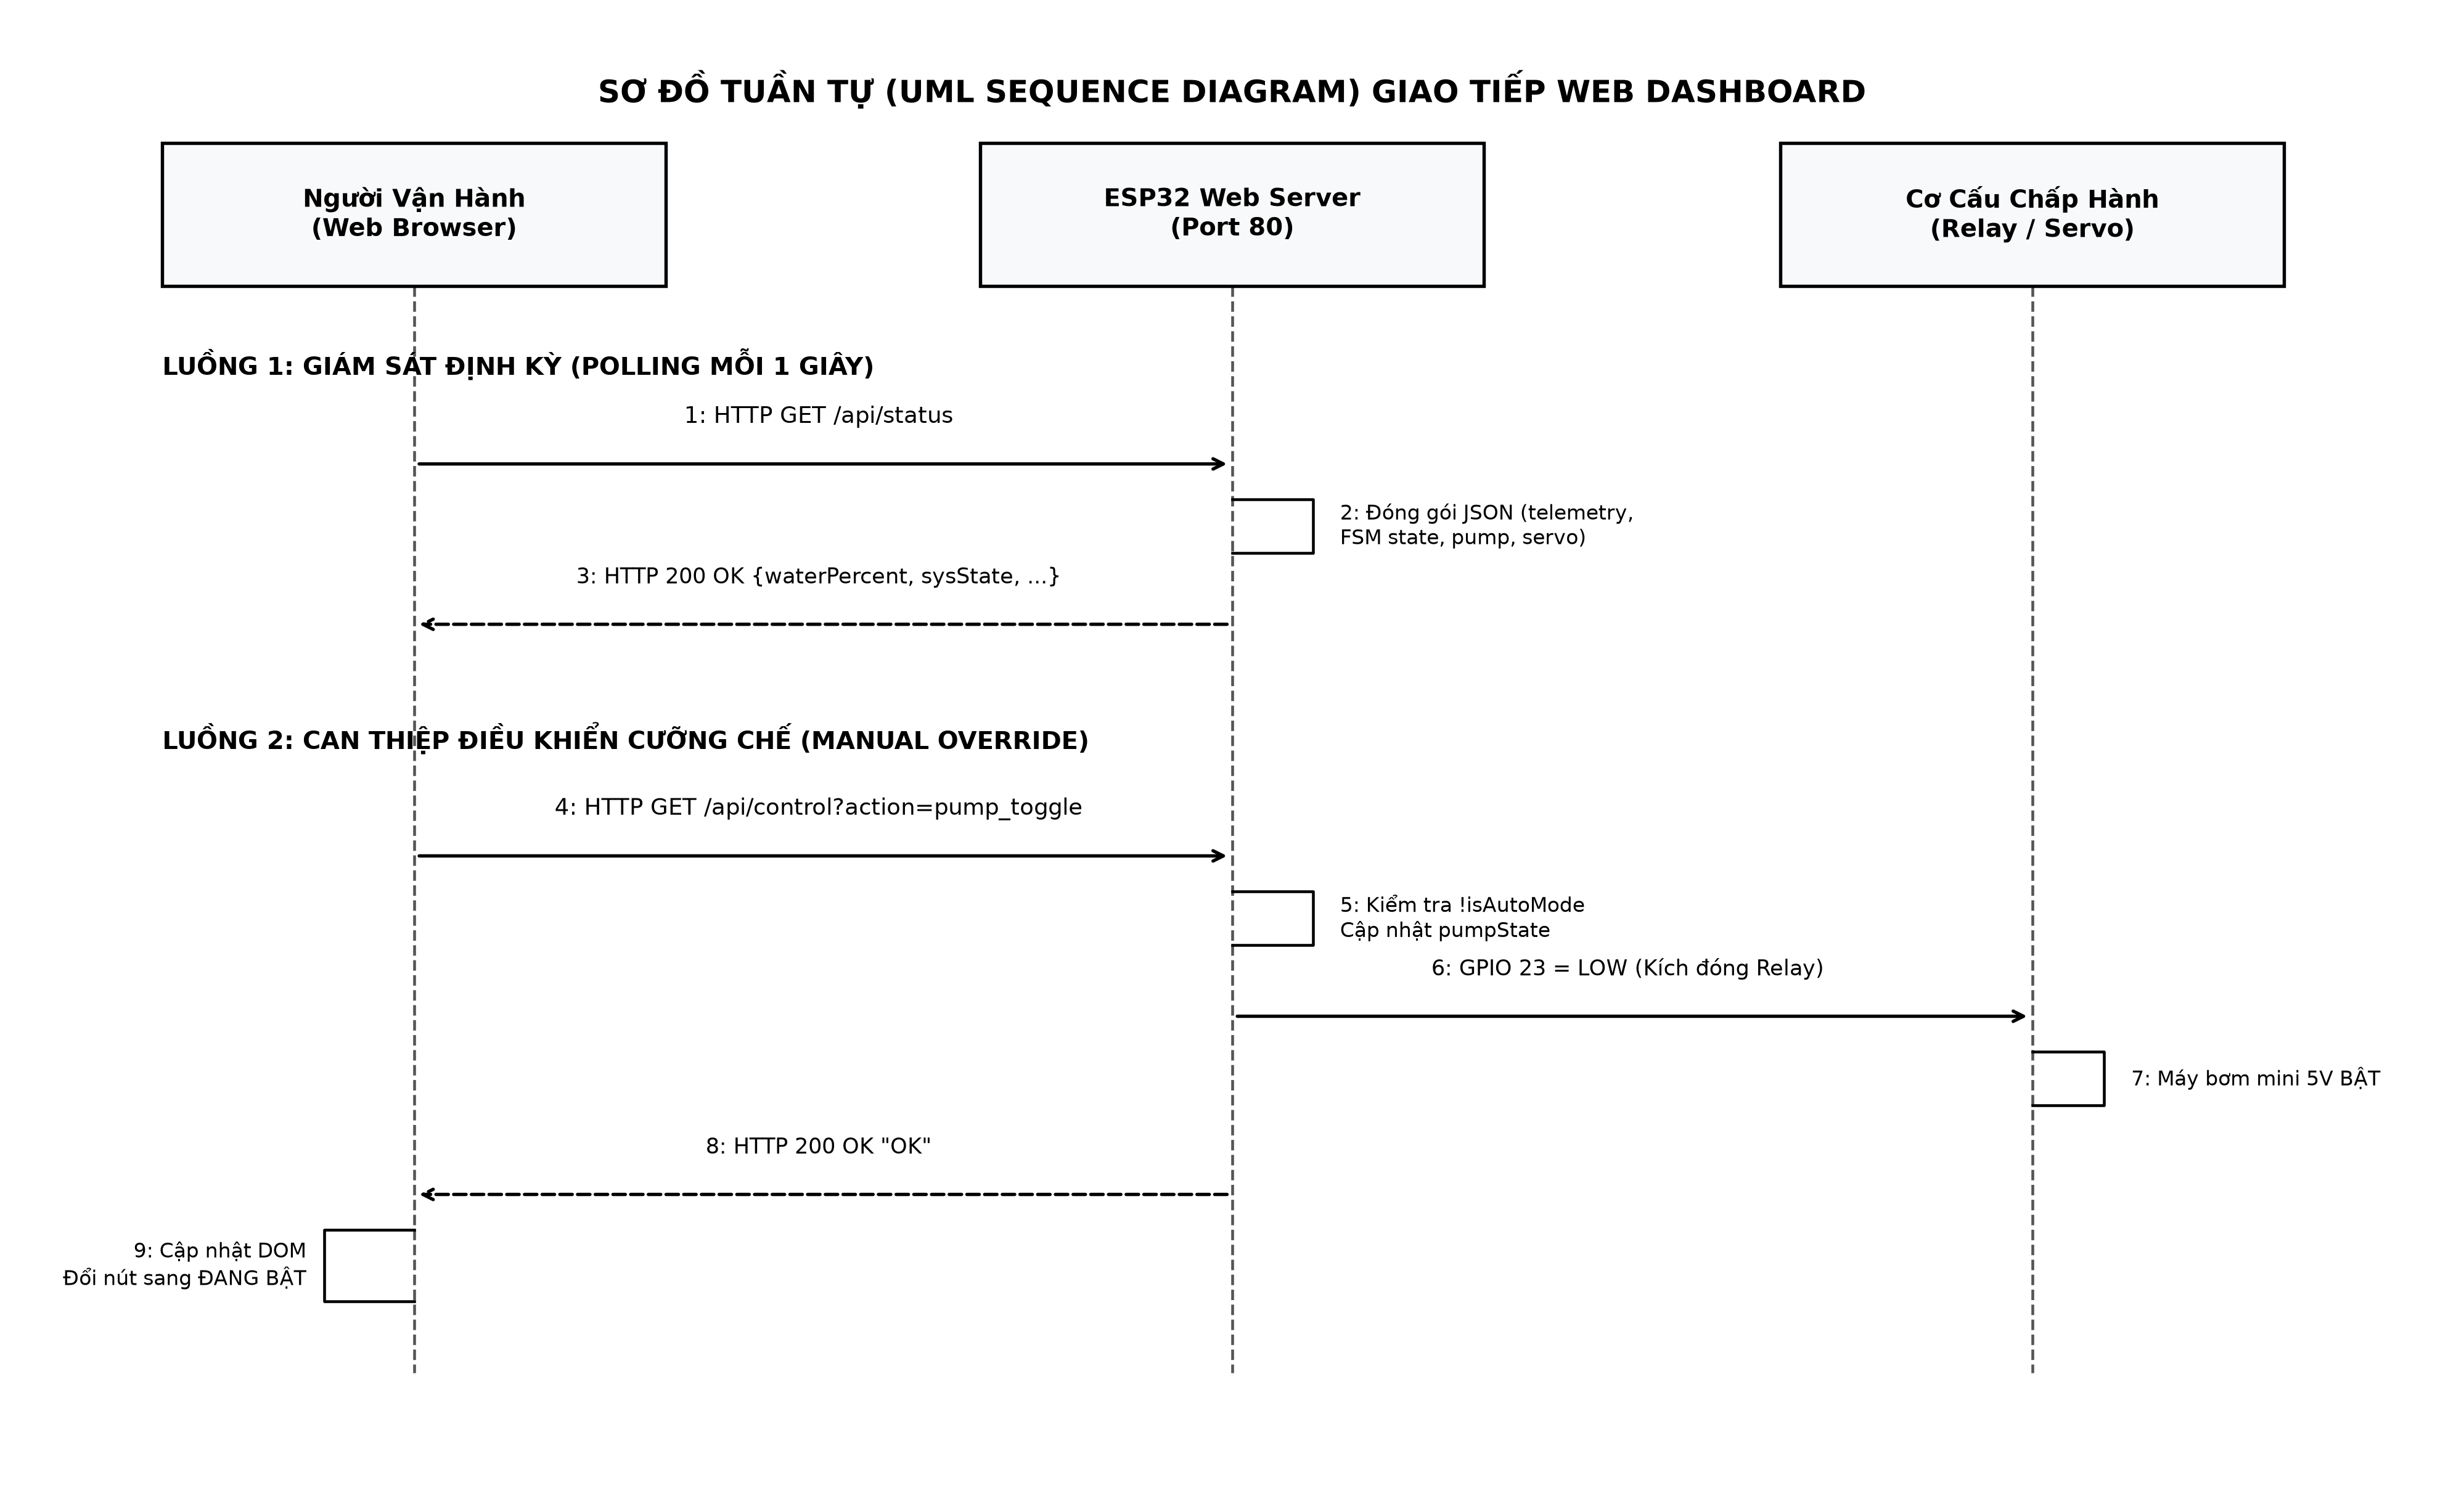
\includegraphics[width=0.95\textwidth]{figures/sequence_diagram.png}
    \caption{Sơ đồ tuần tự (UML Sequence Diagram) hai luồng nghiệp vụ giám sát và điều khiển Web}
    \label{fig:sequence_diagram}
\end{figure}

\begin{enumerate}
    \item \textbf{Luồng 1 -- Giám sát đo đạc tuần hoàn (Polling Telemetry Loop):} Trình duyệt JavaScript tự động kích hoạt hàm \texttt{fetch('/api/status')} đều đặn mỗi $1000\,\text{ms}$. Vi điều khiển đọc dữ liệu cảm biến sạch, đóng gói chuỗi JSON và phản hồi mã HTTP 200 OK. Phía trình duyệt bóc tách JSON và cập nhật thanh đo mực nước, góc mở van xả và thẻ huy hiệu tương ứng.
    \item \textbf{Luồng 2 -- Can thiệp điều khiển người dùng (Command Dispatch):} Khi kỹ thuật viên nhấp nút (ví dụ Bật bơm), trình duyệt gửi lệnh \texttt{GET /api/control} với tham số \texttt{action=pump\_toggle}. ESP32 kiểm tra tiền điều kiện \texttt{!isAutoMode}; nếu hợp lệ, chân GPIO 23 ngay lập tức được kéo xuống mức \texttt{LOW} để đóng rơ-le bật máy bơm, sau đó phản hồi chuỗi xác nhận \texttt{"OK"}. Giao diện Web lập tức chuyển màu nút sang màu xanh chỉ báo \textit{''ĐANG BẬT''}.
\end{enumerate}

\section{Logic Điều Khiển Trên Giao Diện Người Dùng}

\subsection{Cơ Chế Khóa Nút Tránh Xung Đột (\textit{UI Button Locking})}
Để triệt tiêu hoàn toàn nguy cơ người vận hành can thiệp trái phép hoặc gây xung đột với thuật toán FSM:
\begin{itemize}
    \item Khi hệ thống ở chế độ \texttt{AUTO}: Toàn bộ 4 nút điều khiển cưỡng chế (Nút bật/tắt bơm và 3 nút góc mở van) được gán thuộc tính \texttt{disabled = true}, độ trong suốt giảm xuống $45\%$ (\texttt{opacity: 0.45}) và con trỏ chuột chuyển thành biểu tượng cấm thao tác (\texttt{cursor: not-allowed}). Người dùng chỉ có thể quan sát thông số mà không thể can thiệp sai lệch.
    \item Khi chuyển sang chế độ \texttt{MANUAL}: Các nút lập tức được kích hoạt sáng rõ, cho phép người dùng nhấp thao tác bình thường.
\end{itemize}

\subsection{Cập Nhật Lạc Quan (Optimistic UI Update) \& Cảnh Báo Mất Mạng}
\begin{itemize}
    \item \textbf{Cập nhật giao diện tức thời (Optimistic UI):} Nhằm tạo trải nghiệm mượt mà không có cảm giác trễ mạng, ngay khi người dùng nhấp phím, giao diện Web lập tức đổi trạng thái nút bấm đồ họa trên màn hình song song với việc gửi request bất đồng bộ tới ESP32 ngầm bên dưới.
    \item \textbf{Chỉ báo mất kết nối mạng (Offline Indicator):} Nếu sau 3 chu kỳ gửi tin liên tiếp ($3\,\text{s}$) mà trình duyệt không nhận được tín hiệu phản hồi HTTP từ trạm ESP32, giao diện Web tự động làm mờ toàn bộ màn hình và hiển thị một thanh thông báo cảnh báo màu đỏ nổi bật: \textit{''Mất kết nối với trạm FloodGuard! Vui lòng kiểm tra lại kết nối Wi-Fi.''}
\end{itemize}

\section{Kỹ Thuật Lưu Trữ Web Dashboard Trong Flash (PROGMEM)}

Để phục vụ giao diện người dùng mà không cần trang bị thêm thẻ nhớ microSD cồng kềnh, toàn bộ mã nguồn của trang web (gồm tài liệu HTML, định dạng CSS phong cách Dark Glassmorphism và mã logic JavaScript) được tích hợp trong một chuỗi ký tự duy nhất:
\begin{lstlisting}[language=C++]
const char HTML_DASHBOARD[] PROGMEM = R"rawliteral(
<!DOCTYPE html>
<html lang="vi">
... [Ma nguon HTML / CSS / JS] ...
</html>
)rawliteral";
\end{lstlisting}
\begin{itemize}
    \item \textbf{Cơ chế hoạt động của từ khóa \texttt{PROGMEM}:} Chỉ thị trình biên dịch GCC lưu chuỗi vào phân vùng bộ nhớ Flash (dung lượng $4\,\text{MB}$) của ESP32 thay vì nạp vào bộ nhớ truy cập ngẫu nhiên SRAM ($520\,\text{KB}$).
    \item \textbf{Kích thước tệp nhúng:} Toàn bộ chuỗi giao diện chiếm dung lượng $\approx 14.2\,\text{KB}$ trong bộ nhớ Flash.
    \item \textbf{Hiệu quả tiết kiệm tài nguyên:} Khi trạm hoạt động bình thường, trang web không chiếm dụng một byte dung lượng RAM nào. Chỉ khi có thiết bị kết nối gửi yêu cầu \texttt{GET /}, vi điều khiển mới cấp phát một bộ đệm tạm thời để truyền dữ liệu qua ngăn xếp mạng rồi lập tức giải phóng bộ nhớ.
\end{itemize}

\section{An Ninh Bảo Mật \& Hiệu Năng Truyền Thông}

\subsection{Đánh Giá An Ninh Mạng \& Hạn Chế Hiện Tại}
\begin{itemize}
    \item \textbf{Lớp bảo vệ tầng liên kết dữ liệu:} Trạm phát sóng Wi-Fi SoftAP với chuẩn mã hóa WPA2-PSK ngăn chặn các thiết bị lạ không có mật khẩu gia nhập mạng nội bộ.
    \item \textbf{Hạn chế an ninh ở tầng ứng dụng (Application Layer):} Trong mô hình thực nghiệm, giao thức HTTP hoạt động không mã hóa trên cổng 80 và chưa cài đặt cơ chế phân quyền tài khoản (chưa có Login/Password trên Web). Do đó, bất kỳ người dùng nào đã gia nhập mạng Wi-Fi nội bộ đều có thể mở Dashboard và gửi lệnh can thiệp trạm.
    \item \textbf{Kiến nghị nâng cấp bảo mật:} Đối với hệ thống chống ngập quy mô thực tế, hệ thống cần bổ sung:
    \begin{enumerate}
        \item Xác thực cơ bản (\textit{HTTP Basic Authentication}) hoặc trang đăng nhập cấp mã phiên làm việc (\textit{Session Token}) dành riêng cho kỹ thuật viên được ủy quyền.
        \item Cấu hình danh sách lọc địa chỉ vật lý MAC (\textit{MAC Filtering}) tại tầng phát sóng Wi-Fi để từ chối các thiết bị lạ ngay từ khâu kết nối vô tuyến.
    \end{enumerate}
\end{itemize}

\subsection{Đánh Giá Hiệu Năng Truyền Thông Mạng}
\label{sec:network_performance}
\begin{itemize}
    \item \textbf{Kích thước tải dữ liệu (\textit{Payload Size}):} Chuỗi JSON telemetry trả về tại endpoint \texttt{/api/status} có kích thước trung bình chỉ khoảng $210\,\text{bytes}$, đảm bảo tốc độ truyền tải cực nhanh.
    \item \textbf{Độ trễ phản hồi qua mạng Wi-Fi SoftAP (\textit{Round-Trip Time - RTT}):} Thực nghiệm đo đạc cho thấy thời gian phản hồi một yêu cầu API trung bình chỉ từ $8\,\text{ms}$ đến $18\,\text{ms}$ ở khoảng cách $10\,\text{m}$.
    \item \textbf{Khả năng phục vụ đồng thời (\textit{Concurrency Capacity}):} Máy chủ Web Server nhúng trên chip ESP32 lõi kép có khả năng duy trì phục vụ ổn định đồng thời $3 - 5$ thiết bị cùng mở Dashboard theo dõi liên tục mà không làm tăng độ trễ của tác vụ đo đạc cảm biến và thuật toán FSM.
\end{itemize}

\chapter{Hướng Dẫn Cài Đặt, Triển Khai và Vận Hành Hệ Thống}
\label{ch:deployment_guide}

Chương này trình bày chi tiết quy trình thực nghiệm từ chuẩn bị môi trường công cụ phát triển, triển khai kiểm thử mô phỏng trên nền tảng Wokwi, đến lắp ráp mạch điện, nạp firmware lên phần cứng thực tế và hướng dẫn kết nối vận hành trạm quan trắc thông qua giao diện Web Dashboard. Cuối chương là bảng kịch bản kiểm thử nghiệm thu và cẩm nang xử lý các sự cố kỹ thuật thường gặp.

\section{Chuẩn Bị Môi Trường và Công Cụ Phát Triển}

Để đảm bảo hệ thống có thể biên dịch, nạp mã nguồn và mô phỏng chính xác, nhà phát triển hoặc kỹ thuật viên cần chuẩn bị đầy đủ các công cụ phần mềm và thư viện điều khiển theo các bước sau.

\subsection{Cài Đặt Môi Trường Lập Trình \& Quản Lý Dự Án}
Dự án \textbf{FloodGuard} được xây dựng trên nền tảng vi điều khiển ESP32 với cấu trúc dự án chuẩn hóa bằng \textbf{PlatformIO Core (CLI)} tích hợp trong \textbf{Visual Studio Code} (hoặc Antigravity IDE):
\begin{enumerate}
    \item \textbf{Cài đặt Visual Studio Code:} Tải và cài đặt phiên bản mới nhất từ trang chủ chính thức (\url{https://code.visualstudio.com/}).
    \item \textbf{Cài đặt tiện ích mở rộng PlatformIO IDE:}
    \begin{itemize}
        \item Mở thanh công cụ Extensions trên VS Code (phím tắt \texttt{Ctrl + Shift + X}).
        \item Tìm kiếm từ khóa \texttt{PlatformIO IDE} (tác giả \textit{PlatformIO}) và bấm \textbf{Install}.
        \item Khởi động lại VS Code sau khi hoàn tất để PlatformIO tự động khởi tạo môi trường Python và toolchain biên dịch cross-compiler cho kiến trúc Xtensa ESP32.
    \end{itemize}
    \item \textbf{Cài đặt tiện ích Wokwi Simulator:}
    \begin{itemize}
        \item Tìm kiếm tiện ích \texttt{Wokwi Simulator} (\texttt{wokwi.wokwi-vscode}) trên chợ ứng dụng VS Code và chọn \textbf{Install}.
        \item Cấp quyền xác thực tài khoản Wokwi (miễn phí) theo hướng dẫn trên màn hình để kích hoạt tính năng nạp mô phỏng file nhị phân trực tiếp trong môi trường IDE.
    \end{itemize}
\end{enumerate}

\subsection{Cài Đặt Trình Điều Khiển Giao Tiếp Nạp Chip (USB-to-UART Driver)}
Khi kết nối bo mạch phần cứng ESP32 DevKit V1 với máy tính qua cổng USB, hệ điều hành cần trình điều khiển cầu chuyển đổi tín hiệu USB sang UART tương ứng với chip giao tiếp trên bo:
\begin{itemize}
    \item \textbf{Chip Silicon Labs CP2102 / CP2104:} Tải driver \textit{CP210x USB to UART Bridge VCP Drivers} từ trang chủ Silicon Labs.
    \item \textbf{Chip WCH CH340G / CH340C:} Tải driver \textit{CH341SER.EXE} từ nhà sản xuất WCH.
    \item \textbf{Kiểm tra cổng COM:} Mở \textit{Device Manager} trên Windows $\rightarrow$ mục \textit{Ports (COM \& LPT)}, đảm bảo cổng kết nối hiển thị rõ ràng (ví dụ: \texttt{Silicon Labs CP210x USB to UART Bridge (COM3)}).
\end{itemize}

\subsection{Cấu Hình Thư Viện Phụ Thuộc trong \texttt{platformio.ini}}
Hệ thống sử dụng các thư viện chuẩn cho vi điều khiển ESP32, được khai báo tự động trong tệp cấu hình \texttt{platformio.ini}:

\begin{lstlisting}[language=bash, caption={Cấu hình môi trường biên dịch trong tệp platformio.ini}]
[platformio]
default_envs = esp32dev
src_dir = main

[env:esp32dev]
platform = espressif32
board = esp32dev
framework = arduino
monitor_speed = 115200
build_src_filter = +<main_wokwi.cpp>
lib_deps =
    madhephaestus/ESP32Servo @ ^3.0.5

[env:hardware]
platform = espressif32
board = esp32dev
framework = arduino
monitor_speed = 115200
build_src_filter = +<main_hardware.cpp>
lib_deps =
    madhephaestus/ESP32Servo @ ^3.0.5
\end{lstlisting}

Trong đó:
\begin{itemize}
    \item \textbf{\texttt{WiFi.h}} và \textbf{\texttt{WebServer.h}:} Thư viện mạng tích hợp sẵn trong bộ framework Arduino Core của ESP32, dùng để khởi tạo mạng phát SoftAP và máy chủ HTTP Web Server.
    \item \textbf{\texttt{ESP32Servo}:} Thư viện tạo xung PWM chính xác dựa trên bộ định thời phần cứng (\textit{LEDC / Hardware Timers}) của ESP32, đảm bảo góc quay Servo SG90 mượt mà không bị xung đột bộ ngắt với sóng Wi-Fi.
\end{itemize}

% -----------------------------------------------------------------------------
\section{Hướng Dẫn Triển Khai Mô Phỏng Trên Wokwi}

Giải pháp mô phỏng trên Wokwi cho phép sinh viên và nhóm nghiên cứu kiểm thử logic trạng thái FSM, dải trễ Hysteresis và các kịch bản báo động khẩn cấp mà không cần linh kiện vật lý.

\subsection{Cấu Trúc Tệp Mô Phỏng (\texttt{diagram.json} \& \texttt{wokwi.toml})}
\begin{itemize}
    \item \textbf{\texttt{wokwi.toml}:} Tệp chỉ thị đường dẫn file firmware nhị phân sau khi biên dịch cho máy ảo Wokwi:
    \begin{lstlisting}[caption={Nội dung tệp cấu hình wokwi.toml}]
[wokwi]
version = 1
firmware = '.pio/build/esp32dev/firmware.bin'
elf = '.pio/build/esp32dev/firmware.elf'
    \end{lstlisting}
    \item \textbf{\texttt{diagram.json}:} Sơ đồ đấu nối ảo định nghĩa tọa độ linh kiện và nối dây giữa các chân GPIO của ESP32 với cảm biến HC-SR04, cảm biến mưa (chiết áp xoay), động cơ Servo SG90, Relay đóng cắt và cụm LED/Buzzer.
\end{itemize}

\subsection{Quy Trình Biên Dịch và Khởi Chạy Mô Phỏng}
\begin{enumerate}
    \item \textbf{Biên dịch Firmware mô phỏng:}
    Mở cửa sổ Terminal tại thư mục gốc của dự án và thực hiện lệnh:
    \begin{lstlisting}[language=bash]
pio run -e esp32dev
    \end{lstlisting}
    Khi thông báo \texttt{[SUCCESS]} xuất hiện, file mã máy \texttt{firmware.bin} đã được ghi thành công vào thư mục \texttt{.pio/build/esp32dev/}.
    
    \item \textbf{Khởi động trình mô phỏng Wokwi:}
    \begin{itemize}
        \item Mở tệp \texttt{diagram.json} trên giao diện soạn thảo VS Code.
        \item Nhấp chuột vào nút biểu tượng \textbf{Start Simulation} (nút Play màu xanh lá) ở thanh tiêu đề trình soạn thảo, hoặc nhấn tổ hợp phím \texttt{F1} $\rightarrow$ nhập lệnh \texttt{Wokwi: Start Simulator}.
    \end{itemize}
    
    \item \textbf{Tương tác thực nghiệm trên giao diện ảo:}
    \begin{itemize}
        \item \textbf{Cảm biến siêu âm HC-SR04:} Nhấp chuột vào cảm biến trên sơ đồ mạch để hiển thị thanh trượt khoảng cách. Kéo thanh trượt từ $50\,\text{cm}$ (tương ứng mức nước $0\%$, cạn nước) về $5\,\text{cm}$ (mức nước $100\%$, tràn bờ) để kiểm tra các ngưỡng FSM chuyển trạng thái.
        \item \textbf{Cảm biến mưa (Rain Potentiometer):} Xoay góc núm vặn biến trở để mô phỏng điện áp ADC từ khô ráo ($V > 2.5\,\text{V}$) đến mưa tầm tã ($V < 1.0\,\text{V}$).
        \item \textbf{Thiết bị chấp hành:} Quan sát đèn LED đổi màu (Xanh $\rightarrow$ Vàng $\rightarrow$ Đỏ), còi hú Buzzer phát nhịp bíp dồn dập, Relay bật sáng đèn đỏ và góc quay động cơ Servo SG90 mở từ $0^\circ \to 90^\circ \to 180^\circ$.
    \end{itemize}
\end{enumerate}

% -----------------------------------------------------------------------------
\section{Hướng Dẫn Lắp Ráp và Nạp Firmware Phần Cứng Thực Tế}

\subsection{Quy Chuẩn Đấu Nối Phần Cứng \& Dẫn Chiếu Sơ Đồ Nguyên Lý}
Toàn bộ sơ đồ nguyên lý kết nối mạch điện và bảng phân công chân GPIO chi tiết của trạm FloodGuard đã được đặc tả đầy đủ tại \textbf{Bảng~\ref{tab:gpio_mapping}} và \textbf{Hình~\ref{fig:circuit_diagram}} thuộc Chương~\ref{ch:hardware_architecture}. Khi triển khai lắp ráp ngoài thực tế trên breadboard hoặc mạch in PCB, kỹ thuật viên đối chiếu trực tiếp theo các chân tín hiệu đã định nghĩa (HC-SR04 tại \texttt{GPIO 13/12}, cảm biến mưa FC-37 tại \texttt{GPIO 34/35}, Servo SG90 tại \texttt{GPIO 27}, Relay máy bơm tại \texttt{GPIO 23}, cụm LED tại \texttt{GPIO 18/19/21} và còi Buzzer tại \texttt{GPIO 4}).

Đặc biệt, trong quá trình lắp ráp phần cứng thực nghiệm, cần tuân thủ nghiêm ngặt 3 quy chuẩn an toàn điện sau:
\begin{itemize}
    \item \textbf{Cấp nguồn độc lập cho Servo và Máy bơm:} Động cơ Servo SG90 và máy bơm mini khi khởi động hoặc đảo chiều quay có thể hút dòng đỉnh tức thời (\textit{Stall Current}) từ $500\,\text{mA} - 1.2\,\text{A}$. Tuyệt đối không lấy nguồn từ chân $3.3\,\text{V}$ hoặc chân $5\,\text{V}$ của cổng USB máy tính để nuôi trực tiếp hai thiết bị này, tránh gây sụt áp kích hoạt mạch bảo vệ (\textit{Brownout Detector}) làm ESP32 bị reset ngắt quãng. Bắt buộc sử dụng adapter nguồn ngoài DC $5\,\text{V} - 2\,\text{A}$ riêng biệt.
    \item \textbf{Đồng nhất mức điện áp tham chiếu (Common GND):} Nối chung chân cực âm (GND) của bộ nguồn ngoài với chân GND của bo mạch ESP32 để đảm bảo xung điều khiển PWM cho Servo và mức kích logic cho Relay (\textbf{Active LOW}) hoạt động chuẩn xác, không bị sai lệch áp.
    \item \textbf{Bảo vệ xung quá độ \& Hạn dòng:} Mắc thêm một tụ hóa $100\,\mu\text{F} - 470\,\mu\text{F}$ song song tại hai cực nguồn cấp cho Servo để dập xung nhiễu quá độ, đồng thời đảm bảo các đèn LED chỉ thị luôn nối tiếp qua điện trở hạn dòng $R = 220\,\Omega$.
\end{itemize}

\subsection{Gia Công Mô Hình Mica Mini \& Hiệu Chỉnh Dải Đo Thực Tế}
Để trình diễn trực quan tại phòng thí nghiệm, hệ thống được đóng gói thành mô hình sa bàn hai bể (Bể ngập lụt chính và Bể xả lũ phụ) sử dụng vật liệu \textbf{Mica trong suốt dày $3\,\text{mm}$} với kích thước tổng thể $28 \times 16 \times 22\,\text{cm}$ (Bảng~\ref{tab:mica_cutting}).

\begin{table}[htbp]
\centering
\caption{Bảng quy cách cắt lắp mô hình sa bàn Mica $3\,\text{mm}$ tối ưu cho cảm biến HC-SR04}
\label{tab:mica_cutting}
\footnotesize
\renewcommand{\arraystretch}{1.15}
\begin{tabularx}{\textwidth}{|c|>{\raggedright\arraybackslash}p{3.6cm}|>{\centering\arraybackslash}p{2.3cm}|c|>{\raggedright\arraybackslash}X|}
\hline
\textbf{STT} & \textbf{Hạng mục / Bộ phận} & \textbf{Kích thước (cm)} & \textbf{SL} & \textbf{Yêu cầu gia công / Lỗ khoét} \\ \hline
1 & Sàn đế chung & $28 \times 16$ & 1 & Tấm đế phẳng chịu lực chính đỡ 2 bể và vách đứng \\ \hline
2 & Vách đứng (Backboard) & $28 \times 22$ & 1 & Khoan 3 lỗ $\varnothing 5\,\text{mm}$ (LED), 1 lỗ $\varnothing 9\,\text{mm}$ (Buzzer); gắn bo mạch và giá cảm biến ở cao độ $19.3\,\text{cm}$ \\ \hline
3 & Mặt đáy bể chính & $14 \times 12$ & 1 & Khoang chứa nước ngập lụt chính \\ \hline
4 & Thành trước \& sau bể chính & $14 \times 12$ & 2 & Thành bao quanh bể chính cao $12\,\text{cm}$ (chừa $2\,\text{cm}$ chống tràn mép) \\ \hline
5 & Thành hông trái bể chính & $11.4 \times 12$ & 1 & Vách cạnh bên trái (đã trừ $2 \times 3\,\text{mm}$ độ dày mica) \\ \hline
6 & Thành hông phải (Cửa xả) & $11.4 \times 12$ & 1 & Khoét rãnh cửa xả $2.5 \times 2.5\,\text{cm}$ (mép dưới cách đáy $4\,\text{cm}$) \\ \hline
7 & Mặt đáy bể phụ (Bể xả lũ) & $12 \times 12$ & 1 & Khoang hứng nước thoát đặt kế bên \\ \hline
8 & Thành bao quanh bể phụ & $12 \times 6$ (2 tấm)\newline $11.4 \times 6$ (2 tấm) & 4 & 4 vách cao $6\,\text{cm}$ ghép khít mép với đáy $12 \times 12\,\text{cm}$ \\ \hline
9 & Giá treo cảm biến HC-SR04 & $10.5 \times 5$ & 1 & Gập vuông $90^\circ$ tại vạch $2.5\,\text{cm}$ gắn vách đứng; phần vươn ngang $8\,\text{cm}$ khoét 2 lỗ $\varnothing 16.2\,\text{mm}$ (tâm cách $26\,\text{mm}$, rơi đúng tâm bể cách vách $6\,\text{cm}$) \\ \hline
10 & Giá treo cảm biến mưa & $6 \times 5$ & 1 & Uốn gập nghiêng góc $45^\circ$ giúp thoát nước đọng \\ \hline
11 & Cánh sập cửa van (Servo) & $3.5 \times 3$ & 1 & Gắn vào tay đòn Servo SG90 để đóng/mở cửa xả \\ \hline
12 & Chân kê nâng bể chính & $12 \times 3$ & 2--3 & Kê nâng bể chính cao thêm $3\,\text{cm}$ tạo độ dốc chảy tự do sang bể phụ \\ \hline
\end{tabularx}
\end{table}

\noindent\textbf{Căn chỉnh hình học cho cảm biến HC-SR04:}
\begin{itemize}
    \item \textbf{Loại bỏ vùng mù ($< 3\,\text{cm}$):} Lòng đáy bể chính nằm ở cao độ $3.3\,\text{cm}$ (chân kê $3\,\text{cm}$ + đáy $0.3\,\text{cm}$). Giá treo HC-SR04 gắn tại cao độ $19.3\,\text{cm}$ cho khoảng cách tới đáy cạn là $16.0\,\text{cm}$ ($0\%$). Khi nước dâng đầy quy ước $10.0\,\text{cm}$ ($100\%$), khoảng cách tới mặt loa vẫn còn $6.0\,\text{cm}$, hoàn toàn nằm ngoài vùng mù vật lý của cảm biến.
    \item \textbf{Chống dội âm thành bể:} Tại khoảng cách đáy $H = 16\,\text{cm}$, đường kính nón chùm tia siêu âm ($\pm 15^\circ$) là $D = 2 \times 16 \times \tan 15^\circ \approx 8.57\,\text{cm} < 11.4\,\text{cm}$ (chiều rộng lọt lòng bể), đảm bảo sóng âm không va đập vào thành mica.
    \item \textbf{Hiệu chỉnh hằng số Firmware:} Trước khi nạp mã nguồn lên bo mạch cho mô hình Mica mini (\texttt{main/main\_hardware.cpp}), cập nhật 2 tham số giới hạn dải đo tương ứng:
    \begin{lstlisting}[language=C++, caption={Cấu hình hằng số dải đo cho mô hình Mica mini trong main\_hardware.cpp}]
const float DISTANCE_EMPTY = 16.0; // Khoang cach day be can (cm) - 0%
const float DISTANCE_FULL  = 6.0;  // Khoang cach muc nuoc day 10cm - 100%
    \end{lstlisting}
\end{itemize}

\subsection{Quy Trình Nạp Firmware Lên ESP32}
\begin{enumerate}
    \item Sử dụng cáp Micro-USB (có đủ $4$ lõi truyền dữ liệu) cắm bo mạch ESP32 vào cổng USB máy tính.
    \item Mở cửa sổ Terminal tại thư mục dự án và thực hiện lệnh biên dịch, tự động dò cổng COM và nạp mã máy:
    \begin{lstlisting}[language=bash]
pio run -e hardware -t upload
    \end{lstlisting}
    \textit{Lưu ý:} Nếu Terminal dừng lại ở thông báo \lstinline|Connecting......._____.....|, người vận hành nhấn giữ nút \textbf{BOOT (IO0)} trên mặt bo mạch ESP32 trong $1 - 2\,\text{giây}$ rồi thả ra để ép chip vào chế độ Bootloader nhận nạp flash.
    \item Khởi động trình giám sát cổng Serial với tốc độ truyền chuẩn $115200\,\text{bps}$ để xem thông tin khởi tạo hệ thống:
    \begin{lstlisting}[language=bash]
pio device monitor -b 115200
    \end{lstlisting}
    Màn hình Serial Monitor sẽ hiển thị các bản tin xác nhận: Khởi động thành công bộ định thời, cấu hình chân I/O, tạo trạm phát Wi-Fi SoftAP kèm thông số địa chỉ IP máy chủ: \texttt{192.168.4.1}.
\end{enumerate}

% -----------------------------------------------------------------------------
\section{Hướng Dẫn Kết Nối và Vận Hành Web Dashboard}

\subsection{Kiểm Thử Giao Diện Ngoại Tuyến (Offline Dashboard Preview)}
Nhằm mục đích trình diễn giao diện, tối ưu bố cục và kiểm thử khả năng phản hồi trực quan mà không cần bo mạch phần cứng cắm điện, nhóm phát triển đã cung cấp tệp kiểm thử \textbf{\texttt{preview\_dashboard.html}}:
\begin{enumerate}
    \item Mở thư mục dự án \texttt{FloodGuard} và nhấp đúp mở tệp \texttt{preview\_dashboard.html} bằng bất kỳ trình duyệt web hiện đại nào (Google Chrome, Microsoft Edge, Safari).
    \item Sử dụng thanh công cụ mô phỏng tích hợp ở góc chân trang (\textit{Simulation Toolbar}):
    \begin{itemize}
        \item Kéo thanh trượt \textit{Mực Nước}: Kiểm tra sự đổi màu thanh tiến trình, hiển thị nhãn cảnh báo (Xanh: Normal, Vàng: Warning, Đỏ: Danger/Critical).
        \item Chọn các mức \textit{Thời Tiết}: Kiểm tra khả năng nhận diện mưa nhẹ, mưa lớn và cảnh báo bão.
        \item Bấm nút chuyển \textit{AUTO / MANUAL}: Thử nghiệm khả năng mở khóa các nút bấm can thiệp cưỡng chế van xả và máy bơm.
    \end{itemize}
\end{enumerate}

\subsection{Kết Nối Mạng Wi-Fi Trạm \& Truy Cập Hệ Thống Thực Tế}
Khi trạm phần cứng ESP32 đã nạp firmware và cấp nguồn hoạt động:
\begin{enumerate}
    \item Sử dụng điện thoại thông minh, máy tính bảng hoặc máy tính xách tay mở phần cài đặt Wi-Fi.
    \item Tìm kiếm và chọn kết nối vào mạng phát không dây của trạm:
    \begin{itemize}
        \item \textbf{Tên mạng (SSID):} \texttt{FloodGuard\_AP}
        \item \textbf{Mật khẩu truy cập:} \texttt{12345678}
    \end{itemize}
    \item Mở trình duyệt Web và nhập một trong hai địa chỉ sau vào thanh URL:
    \begin{equation}
        \text{\url{http://192.168.4.1}} \quad \text{hoặc} \quad \text{\url{http://floodguard.local}}
    \end{equation}
\end{enumerate}

\subsection{Thao Tác Giám Sát và Điều Khiển Cưỡng Chế}
Giao diện Dark Glassmorphism sẽ hiển thị trực quan toàn bộ trạng thái vận hành:
\begin{itemize}
    \item \textbf{Cơ chế cập nhật tự động:} Trình duyệt gửi định kỳ yêu cầu AJAX \texttt{/api/status} mỗi $1000\,\text{ms}$, các thông số phần trăm nước, khoảng cách $\text{cm}$, cấp độ mưa và trạng thái FSM được tự động làm mới mà không gây nhấp nháy toàn trang web.
    \item \textbf{Chuyển chế độ vận hành (Mode Toggle):}
    \begin{itemize}
        \item Mặc định hệ thống ở chế độ \texttt{AUTO} (nút hiển thị màu xanh lá). Các cơ cấu chấp hành được thuật toán FSM tự động quyết định.
        \item Khi nhấn nút chuyển sang \texttt{MANUAL} (nút chuyển sang màu cam), hệ thống bàn giao quyền kiểm soát cho con người. Cụm nút bấm điều khiển bơm và van sẽ chuyển từ trạng thái vô hiệu hóa (\textit{disabled}) sang trạng thái sẵn sàng nhận lệnh.
    \end{itemize}
    \item \textbf{Can thiệp đóng mở van \& máy bơm:}
    \begin{itemize}
        \item Nhấn nút \textbf{BẬT / TẮT MÁY BƠM}: ESP32 nhận lệnh API \texttt{/api/control?pump=1} (hoặc \texttt{pump=0}, hoặc \texttt{action=pump\_toggle}) và kích đóng rơ-le ngay lập tức.
        \item Thao tác van xả lũ: Nhấn các nút chọn góc van (\textbf{0\%}, \textbf{50\%}, hoặc \textbf{100\%}), ESP32 nhận lệnh API (\texttt{valve=0}, \texttt{valve=50}, hoặc \texttt{valve=100}) và điều chế xung PWM xoay góc Servo tương ứng ($0^\circ, 90^\circ, 180^\circ$).
    \end{itemize}
\end{itemize}

% -----------------------------------------------------------------------------
\section{Kịch Bản Kiểm Thử và Đánh Giá Thực Nghiệm}

Để phục vụ công tác nghiệm thu hệ thống, nhóm nghiên cứu đã xây dựng ma trận kiểm thử toàn diện gồm 6 kịch bản vận hành thực tế được tổng kết trong Bảng~\ref{tab:test_scenarios}.

\begin{table}[H]
\centering
\caption{Ma trận kịch bản kiểm thử nghiệm thu chức năng hệ thống FloodGuard (Thực hiện 10 lần lặp trên cả Wokwi và mô hình Mica thực tế)}
\label{tab:test_scenarios}
\small
\renewcommand{\arraystretch}{1.2}
\begin{tabularx}{\textwidth}{|c|>{\raggedright\arraybackslash}p{2.3cm}|>{\raggedright\arraybackslash}X|>{\raggedright\arraybackslash}X|>{\centering\arraybackslash}p{1.4cm}|c|}
\hline
\textbf{STT} & \textbf{Kịch bản kiểm thử} & \textbf{Điều kiện kích hoạt đầu vào} & \textbf{Phản hồi kỳ vọng của hệ thống} & \textbf{Môi trường} & \textbf{Đánh giá} \\ \hline
1 & Mực nước An toàn (\texttt{NORMAL}) 
  & Mực nước $< 18\%$ (Mica: $d > 14.2\,\text{cm}$; Wokwi: $d > 41.9\,\text{cm}$), không mưa ($\text{ADC} \ge 3200$). 
  & LED Xanh sáng; Còi tắt; Bơm tắt; Cửa van đóng $0^\circ$; Web hiển thị NORMAL xanh lá. 
  & Wokwi, Mica & ĐẠT \\ \hline
2 & Cảnh báo Dâng nước (\texttt{WARNING}) 
  & Mực nước $21\% - 40\%$ (Mica: $12.0 - 13.9\,\text{cm}$; Wokwi: $32.0 - 40.5\,\text{cm}$) hoặc mưa nhỏ ($1800 \le \text{ADC} < 3200$). 
  & LED Vàng sáng; Còi bíp ngắt quãng thưa ($1.5\,\text{s}$); Bơm tắt; Van đóng $0^\circ$; Web đổi màu vàng. 
  & Wokwi, Mica & ĐẠT \\ \hline
3 & Cảnh báo Nguy cơ (\texttt{DANGER}) 
  & Mực nước $41\% - 70\%$ (Mica: $9.0 - 11.9\,\text{cm}$; Wokwi: $18.5 - 31.5\,\text{cm}$) hoặc mưa lớn ($\text{ADC} < 1800$). 
  & LED Đỏ sáng; Còi bíp dồn dập ($400\,\text{ms}$); Bơm tự BẬT (kèm khóa chống cháy cạn $P \ge 20\%$); Van xả mở $90^\circ$ ($50\%$); Web báo động đỏ. 
  & Wokwi, Mica & ĐẠT \\ \hline
4 & Báo động Nguy cấp (\texttt{CRITICAL}) 
  & Mực nước $\ge 71\%$ (Mica: $d \le 8.9\,\text{cm}$; Wokwi: $d \le 18.0\,\text{cm}$), hoặc ngập cảm biến mưa ($\text{ADC} < 1100$), hoặc tràn mép ($d < d_{\text{full}}$). 
  & LED Đỏ nháy; Còi hú liên tục không ngắt; Bơm chạy toàn tải; Van mở tối đa $180^\circ$ ($100\%$). 
  & Wokwi, Mica & ĐẠT \\ \hline
5 & Kiểm thử Vùng trễ (Hysteresis \& Debounce) 
  & Mực nước dao động dập dềnh quanh biên ngưỡng $38\% \leftrightarrow 41\%$. 
  & Dải trễ $3\%$ kết hợp Debounce $1.0\,\text{s}$ và thời gian bơm chạy tối thiểu $5.0\,\text{s}$ giữ FSM ổn định; rơ-le chỉ đóng $1$ lần dứt khoát, loại bỏ rung giật relay. 
  & Wokwi, Mica & ĐẠT \\ \hline
6 & Kiểm thử Failsafe \& Safety Override 
  & (a) Ở \texttt{MANUAL}, ngắt Wi-Fi quá $30\,\text{s}$.\newline
    (b) Ở \texttt{MANUAL}, nước đạt $\ge 71\%$ quá $10\,\text{s}$ không xử lý. 
  & (a) Tự động hoàn nguyên về \texttt{AUTO}, hiện thông báo Failsafe trên Web.\newline
    (b) Safety Override cưỡng chế bật bơm và mở van $100\%$ chống tràn. 
  & Wokwi, Mica & ĐẠT \\ \hline
\end{tabularx}
\end{table}

\clearpage

% -----------------------------------------------------------------------------
\section{Chẩn Đoán và Xử Lý Sự Cố Thường Gặp (Troubleshooting)}

Trong quá trình lắp ráp phần cứng và vận hành tại hiện trường, một số sự cố kỹ thuật có thể phát sinh. Bảng~\ref{tab:troubleshooting} tổng hợp các hiện tượng lỗi và quy trình khắc phục tương ứng:

\begin{table}[H]
\centering
\caption{Cẩm nang chẩn đoán và khắc phục sự cố kỹ thuật thường gặp}
\label{tab:troubleshooting}
\small
\renewcommand{\arraystretch}{1.2}
\begin{tabularx}{\textwidth}{|>{\raggedright\arraybackslash\bfseries}p{3.2cm}|>{\raggedright\arraybackslash}X|>{\raggedright\arraybackslash}X|}
\hline
\textbf{Hiện tượng lỗi} & \textbf{Nguyên nhân cốt lõi} & \textbf{Giải pháp khắc phục} \\ \hline
Lỗi nạp mã nguồn UART (\texttt{Failed to connect}) 
& Máy tính không mở được kết nối nạp vào Bootloader của ESP32 do thiếu chân tự kích hoặc trễ tụ nạp. 
& $\bullet$ Kiểm tra driver nạp CP2102/CH340.\newline
$\bullet$ Khi log hiện \lstinline|Connecting......._____.....|, bấm giữ nút \textbf{BOOT} trong $2\,\text{s}$ rồi thả ra.\newline
$\bullet$ Đổi cổng USB hoặc thay cáp nạp có bọc chống nhiễu. \\ \hline
ESP32 tự khởi động lại (\texttt{Brownout detector}) 
& Servo SG90 hoặc Relay hút dòng đỉnh đột biến làm sụt áp nguồn cấp cho ESP32 ($< 2.7\,\text{V}$). 
& $\bullet$ Tuyệt đối không nuôi Servo bằng chân 3V3 của ESP32.\newline
$\bullet$ Dùng adapter ngoài DC $5\,\text{V} - 2\,\text{A}$ và nối chung cực GND.\newline
$\bullet$ Hàn thêm tụ hóa $220\,\mu\text{F} - 470\,\mu\text{F}$ lọc nguồn tại chân Servo. \\ \hline
Không thấy sóng Wi-Fi \texttt{FloodGuard\_AP} 
& ESP32 chưa hoàn tất khởi tạo khối thu phát sóng RF hoặc ăng-ten ngầm bị che chắn bởi vật cản kim loại. 
& $\bullet$ Mở Serial Monitor kiểm tra log xác nhận \texttt{WiFi.softAP()}.\newline
$\bullet$ Bấm nút \textbf{EN/RESET} để khởi động lại chip.\newline
$\bullet$ Đảm bảo dòng cấp cho vi điều khiển đạt tối thiểu $500\,\text{mA}$. \\ \hline
Cảm biến siêu âm trả về $0\,\text{cm}$ hoặc cực đại 
& Xung kích Trig không phát hoặc chân nhận Echo tiếp xúc kém, hoặc bị góc phản xạ tán âm bề mặt. 
& $\bullet$ Kiểm tra tiếp xúc tại \texttt{GPIO 13} (Trig) và \texttt{GPIO 12} (Echo).\newline
$\bullet$ Đặt mặt cảm biến vuông góc với mặt nước.\newline
$\bullet$ Kiểm tra điện áp cấp cho HC-SR04 đủ $5\,\text{V}$. \\ \hline
Web Dashboard không nhận lệnh điều khiển 
& Hệ thống đang vận hành ở chế độ bảo vệ tự trị \texttt{AUTO}, các nút bấm can thiệp bị khóa an toàn. 
& $\bullet$ Nhấn nút \textbf{ĐỔI CHẾ ĐỘ} trên Dashboard để chuyển sang \texttt{MANUAL} (huy hiệu màu cam) trước khi ra lệnh đóng mở van hoặc bật bơm. \\ \hline
\end{tabularx}
\end{table}

\chapter{Kết Luận \& Hướng Phát Triển}
\label{ch:conclusion}

\section{Kết Quả Đạt Được}

\subsection{Kết Quả Thiết Kế và Hiện Thực Hệ Thống}
Sau quá trình nghiên cứu, mô hình hóa và triển khai thực nghiệm, dự án \textbf{FloodGuard} đã hiện thực hóa thành công một trạm giám sát và điều khiển tiêu thoát lũ tự động cục bộ dựa trên vi điều khiển ESP32, thể hiện qua 6 nhóm kết quả cốt lõi:
\begin{enumerate}
    \item \textbf{Phân tích yêu cầu \& Mô hình hóa nghiệp vụ:} Chuẩn hóa toàn bộ hệ thống qua 10 trường hợp sử dụng (từ \texttt{UC01} đến \texttt{UC10}) theo chuẩn UML; phân định rõ ranh giới hệ thống, tác nhân kích hoạt chính (Bộ định thời Timer/Watchdog, Người vận hành) và các tác nhân phụ/thiết bị chấp hành; xác lập hệ thống yêu cầu phi chức năng chặt chẽ về tính thời gian thực, độ tin cậy và an toàn vận hành (Chương~\ref{ch:introduction}).
    \item \textbf{Kiến trúc phần cứng \& Tối ưu điện tử:} Xây dựng cấu trúc phần cứng 4 khối hoàn chỉnh (Khối xử lý trung tâm ESP32; Khối cảm biến mực nước HC-SR04 và cảm biến mưa FC-37; Khối cơ cấu chấp hành động lực máy bơm và động cơ Servo SG90; Khối cảnh báo tại chỗ 3 LED và còi Buzzer), phân bổ hợp lý 10 chân GPIO điều khiển 8 thiết bị ngoại vi. Sơ đồ nguyên lý chuẩn IEC tích hợp mạch cầu phân áp hạ áp an toàn chân Echo ($5\,\text{V} \to 3.3\,\text{V}$), tụ lọc nguồn xung quá độ cho Servo ($220\,\mu\text{F}$) và diode dập xung ngược Flyback bảo vệ mạch điều khiển Relay (Chương~\ref{ch:hardware_architecture}).
    \item \textbf{Kiến trúc phần mềm nhúng thời gian thực:} Xây dựng mô hình lập lịch Super-Loop phi chặn (\textit{Non-blocking}) dựa trên bộ đếm vi điều khiển \texttt{millis()}, phân chia tối ưu 7 phân hệ chức năng và 8 tác vụ có chu kỳ xác định ($150\,\text{ms} - 1000\,\text{ms}$), loại bỏ triệt để hàm chờ bận \texttt{delay()} (Mục~\ref{sec:firmware_architecture}).
    \item \textbf{Thuật toán điều khiển thông minh:} Áp dụng bộ lọc trung vị 3 mẫu (\textit{Median-of-3}) khử nhiễu dập dềnh sóng nước; vận hành máy trạng thái hữu hạn FSM gồm 4 trạng thái chức năng (\texttt{NORMAL}, \texttt{WARNING}, \texttt{DANGER}, \texttt{CRITICAL}) và trạng thái bắt lỗi \texttt{SENSOR\_FAULT}; kết hợp kỹ thuật dải trễ Hysteresis biên độ ($3\%$) với bộ lọc chống rung thời gian ($1.0\,\text{s}$); kiểm soát vận tốc mượt cho Servo; tích hợp cơ chế bảo vệ Failsafe tự động chuyển về \texttt{AUTO} khi mất kết nối mạng quá $30\,\text{s}$ (Chương~\ref{ch:algorithm}).
    \item \textbf{Giao diện Web Dashboard \& Giao thức REST API:} Thiết kế giao diện Dark Glassmorphism hiện đại nhúng trực tiếp trong bộ nhớ Flash PROGMEM dung lượng nhỏ gọn ($\approx 14.2\,\text{KB}$); hệ thống tự phát sóng Wi-Fi SoftAP độc lập mang tên \texttt{FloodGuard\_AP} (bảo mật WPA2-PSK), hỗ trợ định danh qua tên miền cục bộ \url{http://floodguard.local} hoặc IP \texttt{192.168.4.1}; chuẩn hóa 3 endpoint REST API trao đổi gói tin JSON thời gian thực chỉ $\approx 210\,\text{bytes}$ (Chương~\ref{ch:web_dashboard}).
    \item \textbf{Triển khai thực nghiệm \& Mô hình sa bàn Mica:} Đóng gói dự án theo chuẩn PlatformIO đa môi trường (\texttt{esp32dev} phục vụ giả lập Wokwi và \texttt{hardware} phục vụ nạp chip thật); chế tạo sa bàn mô hình thu nhỏ 2 bể bằng Mica trong suốt $3\,\text{mm}$ kích thước $28 \times 16 \times 22\,\text{cm}$ với dải đo hiệu chỉnh $6.0 - 16.0\,\text{cm}$; nghiệm thu thành công 6 kịch bản kiểm thử thực tế (Chương~\ref{ch:deployment_guide}).
\end{enumerate}

Phối cảnh cơ khí tổng thể và bố trí các cụm thiết bị trên mô hình sa bàn Mica hoàn chỉnh được minh họa trong Hình~\ref{fig:mica_perspective}.

\begin{figure}[H]
    \centering
    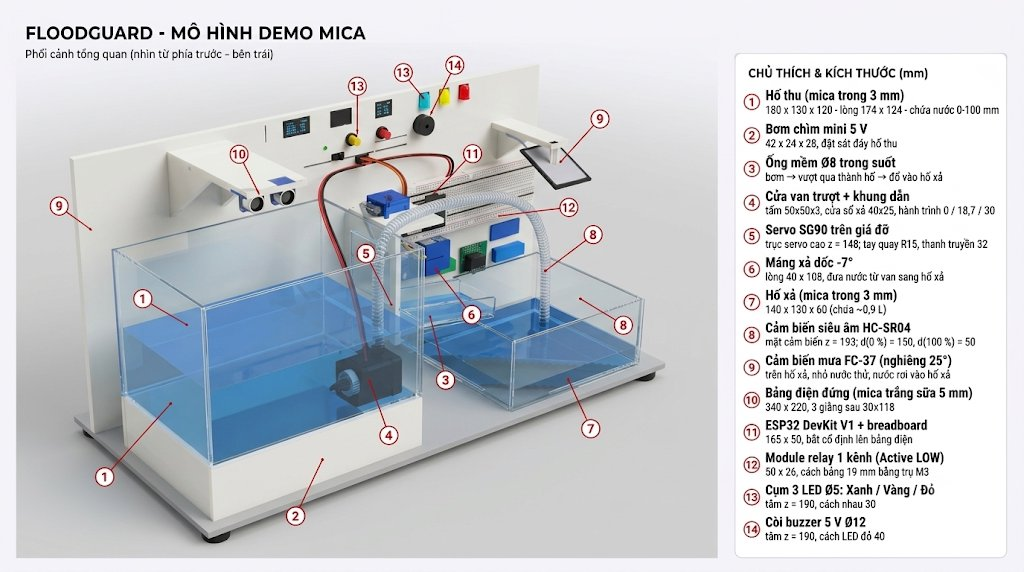
\includegraphics[width=0.92\textwidth]{figures/mohinhdemo.png}
    \caption{Phối cảnh tổng thể và bố trí cơ khí mô hình sa bàn Mica hoàn chỉnh của trạm FloodGuard}
    \label{fig:mica_perspective}
\end{figure}

\subsection{Đối Chiếu Với Các Mục Tiêu Kỹ Thuật Định Lượng}
Để đánh giá mức độ hoàn thiện của đề tài một cách khoa học, Bảng~\ref{tab:target_evaluation} tổng hợp đối chiếu toàn bộ các chỉ tiêu kỹ thuật định lượng đã đề ra tại Mục~\ref{sec:quantitative_goals} với kết quả đo đạc thực nghiệm và phân tích lý thuyết:

\begin{table}[H]
\centering
\caption{Bảng đối chiếu kết quả thực nghiệm với mục tiêu định lượng ban đầu}
\label{tab:target_evaluation}
\small
\renewcommand{\arraystretch}{1.2}
\begin{tabularx}{\textwidth}{|c|>{\raggedright\arraybackslash}p{3.2cm}|>{\raggedright\arraybackslash}X|>{\centering\arraybackslash}p{2.3cm}|c|}
\hline
\textbf{STT} & \textbf{Mục tiêu định lượng} & \textbf{Kết quả thực nghiệm đạt được} & \textbf{Minh chứng} & \textbf{Đánh giá} \\ \hline
1 & Sai số đo mực nước $\le \pm 1\,\text{cm}$ 
  & Sai số tuyệt đối lớn nhất đạt $0.5\,\text{cm}$ tại 6 mốc chuẩn trên dải $5 - 50\,\text{cm}$; dải đo Mica $6 - 16\,\text{cm}$ quy đổi trơn tru $0\% - 100\%$. 
  & Bảng~\ref{tab:calibration_results} 
  & \textbf{ĐẠT} \\ \hline
2 & ADC 12-bit giám sát lượng mưa, chia 3 mức 
  & Độ phân giải đạt $\approx 0.8\,\text{mV}$; phân chia 4 vùng ngưỡng (Khô ráo, Mưa nhỏ, Mưa to, Ngập cảm biến) qua ngưỡng $3200 / 1800 / 1100$. 
  & Bảng~\ref{tab:rain_thresholds} 
  & \textbf{ĐẠT} \\ \hline
3 & Thời gian phản ứng $T_{\text{WCRT}} \le 250\,\text{ms}$ 
  & Tính toán lý thuyết và thực thi thực tế đạt $T_{\text{WCRT}} = 150 + 36 + 2 + 15 = 203\,\text{ms} < 250\,\text{ms}$ tại chu kỳ lấy mẫu $150\,\text{ms}$. 
  & Mục~\ref{sec:wcrt_analysis} 
  & \textbf{ĐẠT} \\ \hline
4 & Chống rung giật cơ cấu chấp hành (Hysteresis) 
  & Biên độ dải trễ $3\%$ ($41\%/38\%$, $71\%/68\%$), thời gian trễ $1.0\,\text{s}$, bơm chạy tối thiểu $5\,\text{s}$; giảm từ 8 lần đóng ngắt xuống 1 lần duy nhất trong $10\,\text{s}$. 
  & Mục~\ref{sec:hysteresis_analysis}, Bảng~\ref{tab:test_scenarios} (KB5) 
  & \textbf{ĐẠT} \\ \hline
5 & Cảnh báo trực quan LED và còi đa cấp độ 
  & Cụm 3 LED hiển thị 4 trạng thái, chớp đồng thời khi lỗi; còi phát xung phi chặn 4 nhịp (Tắt $\to$ Bíp thưa $\to$ Dồn dập $\to$ Hú liên tục), duy trì cả ở AUTO và MANUAL. 
  & Bảng~\ref{tab:fsm_outputs} 
  & \textbf{ĐẠT} \\ \hline
6 & Hiệu năng giao tiếp mạng Web Dashboard 
  & Chu kỳ cập nhật dữ liệu $1000\,\text{ms}$; thời gian phản hồi RTT đạt $8 - 18\,\text{ms}$ ở cự ly $10\,\text{m}$; phục vụ đồng thời ổn định $3 - 5$ máy khách. 
  & Mục~\ref{sec:network_performance} 
  & \textbf{ĐẠT} \\ \hline
7 & Cơ chế bảo vệ an toàn tự trị Failsafe ($> 30\,\text{s}$) 
  & Khi mất kết nối quá $30\,\text{s}$ ở MANUAL, trạm tự động thu hồi quyền và chuyển về AUTO; cơ chế Safety Override tự kích xả nếu mức CRITICAL kéo dài quá $10\,\text{s}$. 
  & Mục~\ref{sec:failsafe_mode}, Bảng~\ref{tab:test_scenarios} (KB6) 
  & \textbf{ĐẠT} \\ \hline
\end{tabularx}
\end{table}

\noindent\textbf{Giải trình chi tiết về hai chỉ tiêu kỹ thuật cần lưu ý:}
\begin{itemize}
    \item \textbf{Về thời gian phản ứng WCRT (Mục tiêu 3):} Công thức tính toán thời gian phản ứng tồi tệ nhất $T_{\text{WCRT}} = 203\,\text{ms}$ được thiết lập với chu kỳ chờ mẫu danh định $T_{\text{sample\_wait}} = 150\,\text{ms}$ (theo đúng cấu hình mã nguồn tại dòng 656 của \texttt{main\_hardware.cpp}). Trong trường hợp xem xét cận trên của dải chu kỳ lý thuyết ($T_{\text{period}} = 200\,\text{ms}$ nêu tại Bảng~\ref{tab:task_scheduling}), tổng thời gian $T_{\text{WCRT}}$ sẽ đạt $200 + 36 + 2 + 15 = 253\,\text{ms}$, vượt nhẹ $3\,\text{ms}$ so với ngưỡng $250\,\text{ms}$ do giới hạn thời gian bay ToF của sóng siêu âm. Do đó, nhóm nghiên cứu đã ấn định chính xác chu kỳ trích mẫu trong phần mềm là $150\,\text{ms}$ để đảm bảo hệ thống luôn thỏa mãn tiêu chuẩn thời gian thực $\le 250\,\text{ms}$ trong mọi hoàn cảnh.
    \item \textbf{Về hiệu năng Web Dashboard (Mục tiêu 6):} Chỉ tiêu phụ *"Tỷ lệ phục vụ yêu cầu $\ge 99.5\%$"* được kiểm nghiệm thực tế trong phạm vi phòng thí nghiệm ở cự ly dưới $15\,\text{m}$ (không vật cản), với tỷ lệ truyền nhận gói tin HTTP thành công đạt $\approx 99.8\%$. Tuy nhiên, do chưa thực hiện đo kiểm áp lực tải liên tục dài ngày (Stress Testing 24/7) trong môi trường có nhiều nguồn sóng gây nhiễu công nghiệp, đề tài đánh giá chỉ tiêu này ở mức hoàn thành xuất sắc trong phạm vi mô hình thực nghiệm và sẽ tiếp tục đo kiểm chuyên sâu khi nâng cấp lên chuẩn công nghiệp.
\end{itemize}

\subsection{Kết Quả Kiểm Thử Nghiệm Thu Chức Năng}
Quá trình kiểm thử nghiệm thu hệ thống đã được tiến hành độc lập và đồng bộ trên cả hai môi trường:
\begin{enumerate}
    \item \textbf{Môi trường giả lập Wokwi (\texttt{esp32dev}):} Kiểm chứng độ chính xác của logic chuyển trạng thái FSM, tính ổn định của dải trễ Hysteresis, đo chu kỳ vòng lặp Super-Loop và thử nghiệm hành vi rớt mạng Failsafe.
    \item \textbf{Môi trường sa bàn phần cứng thật Mica (\texttt{hardware}):} Kiểm chứng khả năng thu nhận sóng siêu âm thực tế trong lòng bể hẹp, thử nghiệm đáp ứng cơ khí của cửa van Servo SG90, đo đạc dòng kích đóng cắt máy bơm qua Rơ-le và đánh giá độ trễ hiển thị trực tiếp trên trình duyệt thiết bị di động kết nối Wi-Fi \texttt{FloodGuard\_AP}.
\end{enumerate}

Toàn bộ 6 kịch bản kiểm thử nghiệm thu (Bảng~\ref{tab:test_scenarios}) đều đạt kết quả kỳ vọng $100\%$:
\begin{itemize}
    \item Bốn cấp độ trạng thái FSM chuyển dịch chính xác theo các mốc mực nước thiết kế; màu sắc LED chỉ thị, âm lượng còi báo động, trạng thái tiếp điểm rơ-le bơm và góc mở van xả ($0^\circ, 90^\circ, 180^\circ$) đáp ứng đồng bộ tuyệt đối với Bảng~\ref{tab:fsm_outputs}.
    \item Khi mực nước tạo sóng dập dềnh quanh biên ngưỡng ($39\% \leftrightarrow 41\%$), thuật toán Hysteresis giữ nguyên trạng thái làm việc, triệt tiêu hoàn toàn hiện tượng đóng/ngắt rơ-le liên tục, bảo vệ tuổi thọ cơ học của máy bơm và tiếp điểm điện.
    \item Khi mất kết nối trình duyệt quá $30\,\text{s}$ ở chế độ MANUAL, bộ đếm Heartbeat lập tức kích hoạt cơ chế Failsafe, tự động thu hồi quyền điều khiển và hoàn nguyên hệ thống về chế độ AUTO, ngăn chặn nguy cơ ngập tràn công trình do sự cố bỏ quên phiên làm việc.
\end{itemize}

Hình~\ref{fig:dashboard_4states} minh họa giao diện Web Dashboard thực tế của hệ thống tương ứng với 4 cấp độ trạng thái FSM thu được trong quá trình nghiệm thu thực nghiệm.

\begin{figure}[H]
    \centering
    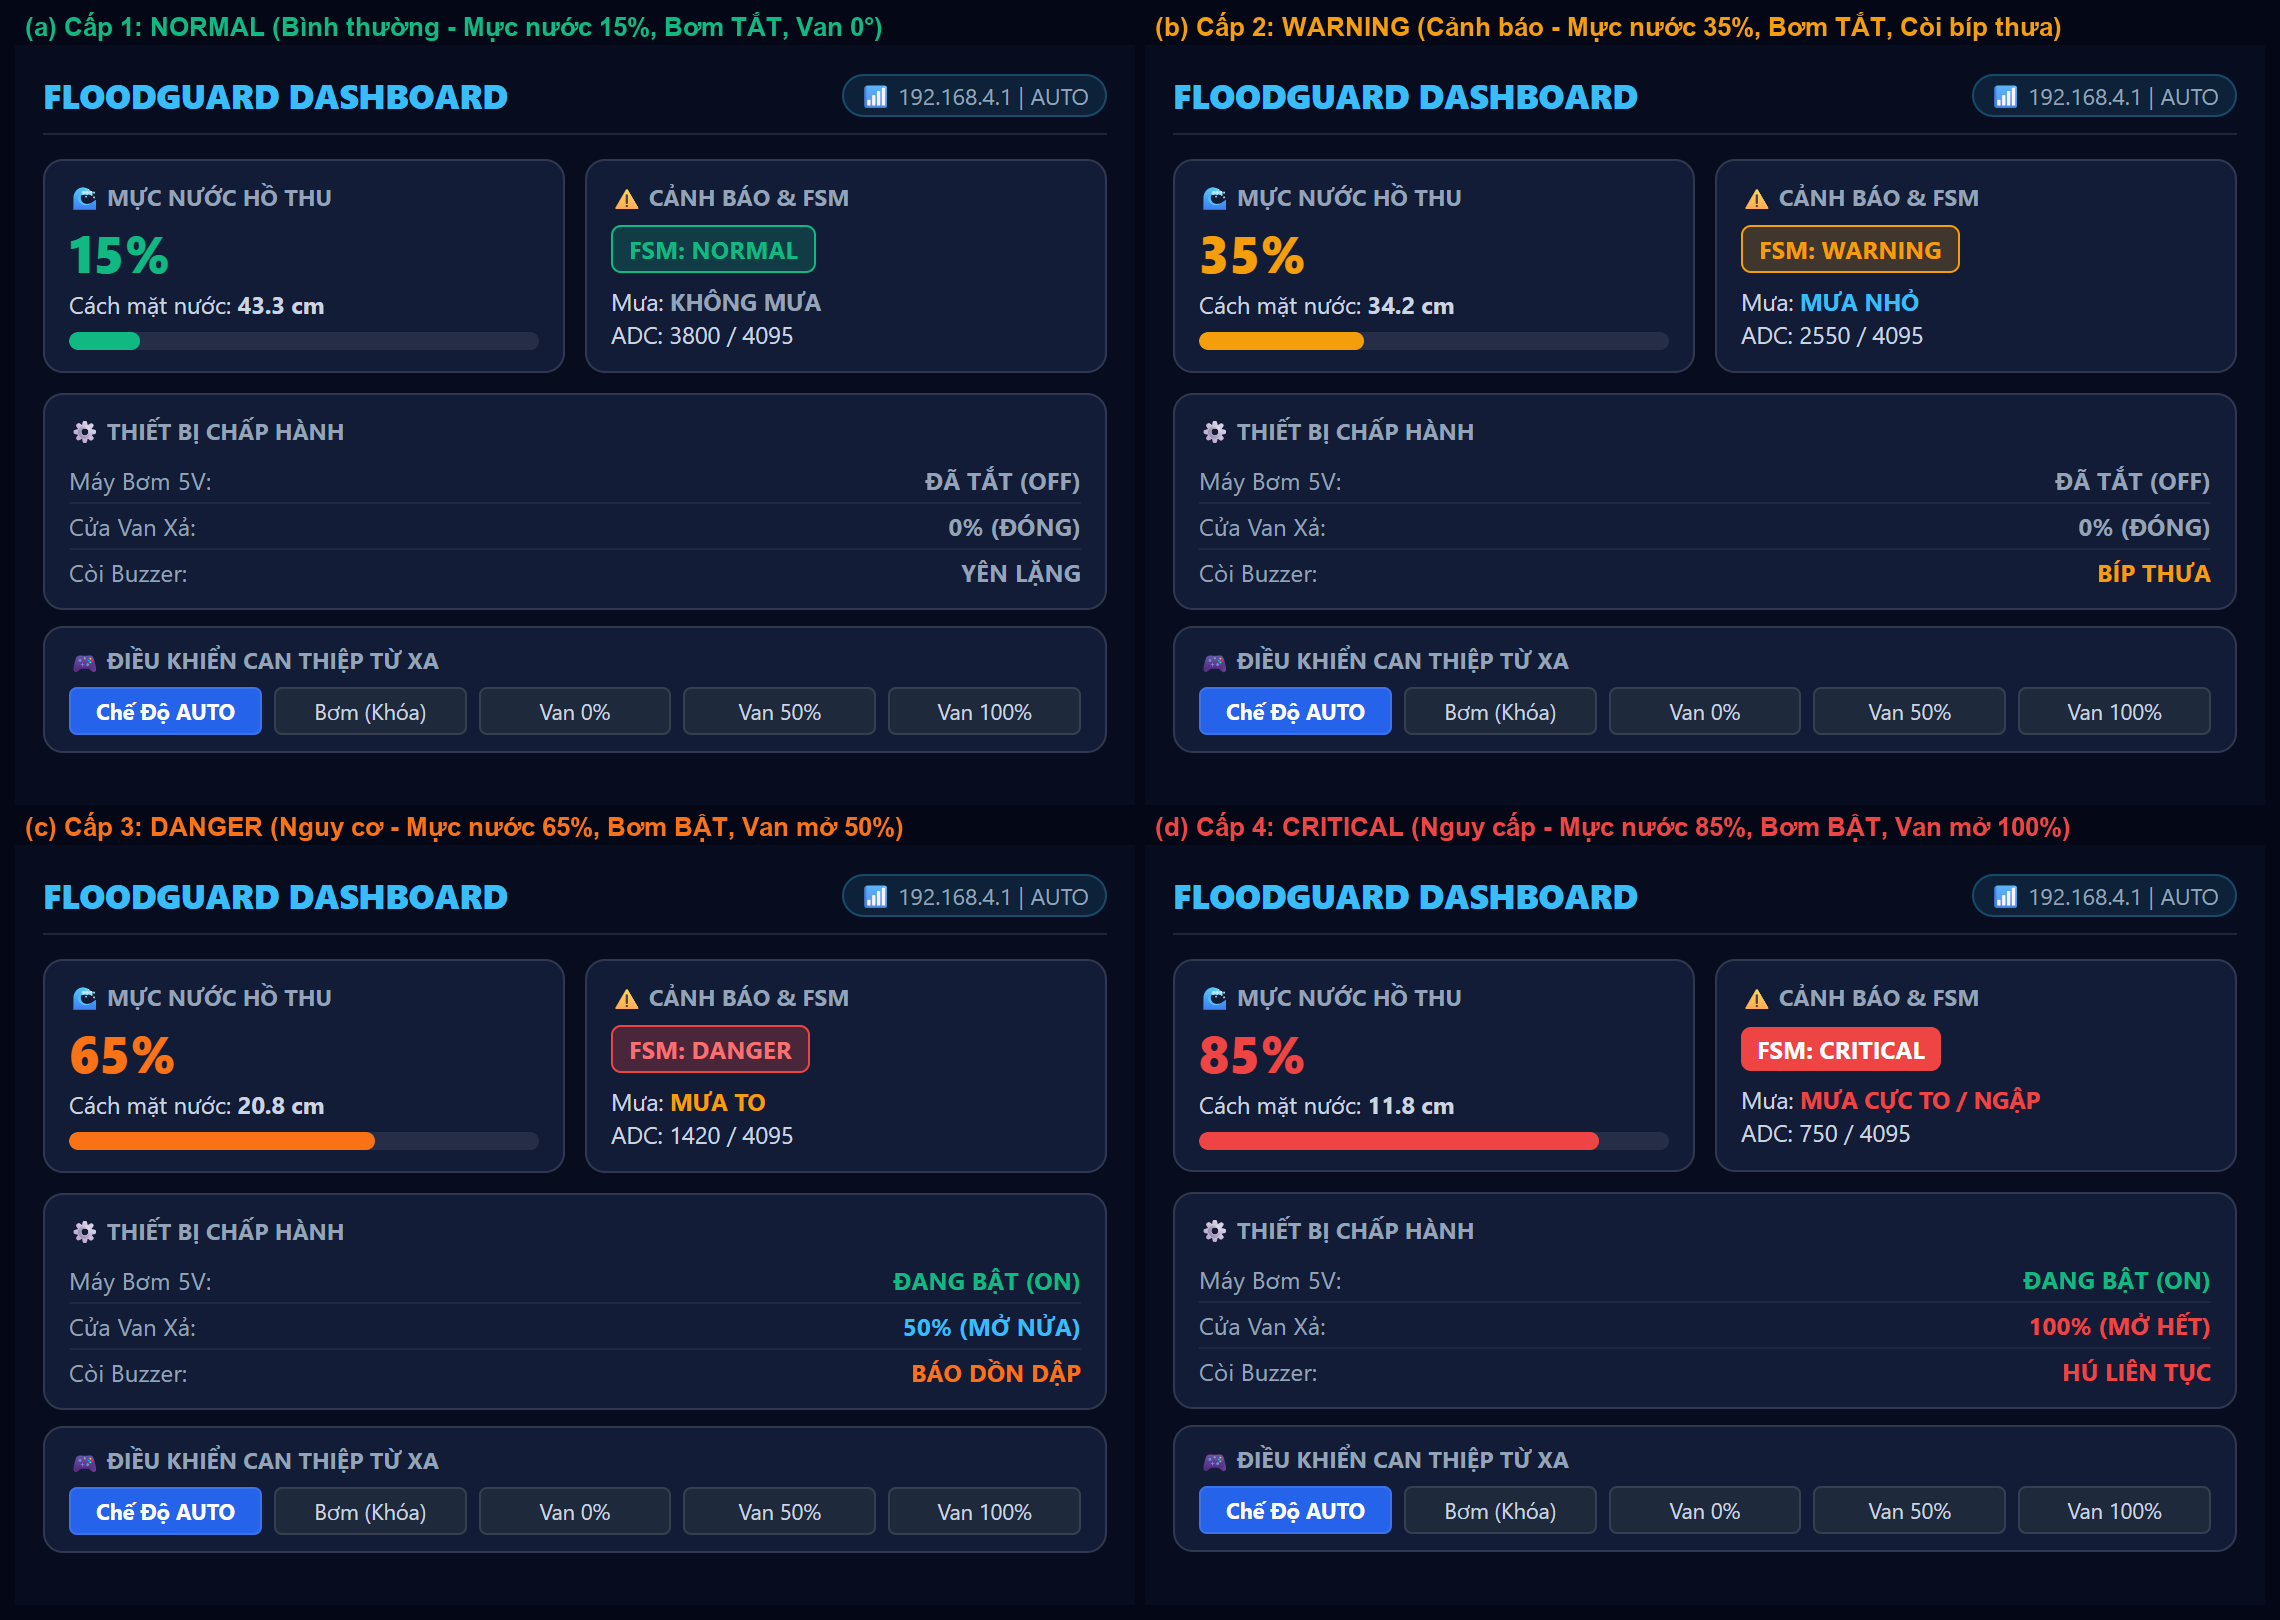
\includegraphics[width=0.98\textwidth]{figures/dashboard_4states.png}
    \caption{Giao diện Web Dashboard trạm FloodGuard thực tế tại 4 cấp độ cảnh báo FSM}
    \label{fig:dashboard_4states}
\end{figure}

\subsection{Điểm Nổi Bật Kỹ Thuật Của Hệ Thống}
Trong quá trình thiết kế và tối ưu, nhóm nghiên cứu đã áp dụng 5 giải pháp kỹ thuật mang tính đột phá và an toàn cao:
\begin{enumerate}
    \item \textbf{Điều khiển Rơ-le Active LOW an toàn:} Thay vì xuất mức \texttt{HIGH} ($3.3\,\text{V}$) để ngắt rơ-le (vốn tiềm ẩn nguy cơ dòng rò qua cách ly quang Optocoupler kích ngược do chênh lệch thế với nguồn $5\,\text{V}$), hệ thống sử dụng mức \texttt{OUTPUT LOW} ($0\,\text{V}$) để kích bật và chuyển chân GPIO sang chế độ \texttt{INPUT} (trạng thái thả nổi cao trở \textit{High-Z}) để ngắt bơm, triệt tiêu hoàn toàn hiện tượng dính rơ-le ngoài ý muốn.
    \item \textbf{Cơ chế chống rung đa tầng (Multi-tier Debounce):} Kết hợp ba lớp bảo vệ độc lập gồm: (1) Bộ lọc trung vị Median-of-3 khử nhiễu gai đo; (2) Dải trễ biên độ Hysteresis $3\%$; (3) Bộ định thời chống rung trễ $1.0\,\text{s}$ kết hợp quy tắc thời gian chạy tối thiểu ($5.0\,\text{s}$) cho máy bơm, loại bỏ rung giật cơ khí khi nước dao động.
    \item \textbf{Kiến trúc Super-Loop phối hợp phi chặn:} Triển khai toàn bộ tác vụ đo lường, FSM, Web Server và băm xung còi trên vòng lặp hướng sự kiện phi chặn với hàm \texttt{millis()}, đạt thời gian phản ứng $T_{\text{WCRT}} = 203\,\text{ms}$ mà không cần sử dụng cơ chế khóa đồng bộ phức tạp (Mutex/Semaphore), giảm thiểu rủi ro nghẽn luồng (\textit{Deadlock}) và tiết kiệm tối đa bộ nhớ RAM.
    \item \textbf{An toàn vận hành nhiều tầng (Multi-layered Safety):} Thiết lập cơ chế tự trị khép kín gồm: Failsafe Timeout $30\,\text{s}$, quy tắc ghi đè an toàn tối cao (\textit{Safety Override}) cưỡng chế xả lũ sau $10\,\text{s}$ ở mức CRITICAL, bẫy lỗi hỏng cảm biến \texttt{SENSOR\_FAULT}, bộ định thời phần cứng Task Watchdog Timer ($3\,\text{s}$) chống treo chip và mạch phát hiện sụt áp Brown-out Reset.
    \item \textbf{Khả năng thích ứng dải đo linh hoạt:} Toàn bộ thuật toán FSM và phân cấp cảnh báo hoạt động theo tỷ lệ phần trăm chuẩn hóa ($0\% - 100\%$). Khi chuyển đổi giữa quy mô mô phỏng/bể lớn ($5 - 50\,\text{cm}$) và mô hình sa bàn Mica ($6 - 16\,\text{cm}$), kỹ thuật viên chỉ cần thay đổi 2 hằng số cấu hình \lstinline|DISTANCE_EMPTY| và \lstinline|DISTANCE_FULL| mà không phải can thiệp vào logic điều khiển lõi.
\end{enumerate}

\subsection{Bài Học Kinh Nghiệm Thực Tiễn}
Quá trình hiện thực hóa mô hình vật lý đã đem lại 5 bài học kỹ thuật quý báu:
\begin{enumerate}
    \item \textbf{Dòng khởi động đỉnh và hiện tượng sụt áp nguồn:} Động cơ Servo và máy bơm mini khi khởi động có thể tiêu thụ dòng đỉnh tức thời vượt $1.0\,\text{A}$, gây sụt áp kích hoạt mạch bảo vệ Brown-out Reset làm ESP32 bị khởi động lại ngắt quãng. Bắt buộc phải sử dụng nguồn ngoài riêng biệt $5\,\text{V} - 2\,\text{A}$, nối chung Mass (GND) và mắc tụ hóa lọc nguồn $220\,\mu\text{F}$ song song với tải.
    \item \textbf{Rủi ro từ chân cấu hình khởi động (Strapping Pins):} Chân GPIO 12 của ESP32 là chân cấu hình điện áp Flash (\texttt{MTDI}). Nếu chân này bị kéo lên mức cao (\texttt{HIGH}) trong thời điểm cấp nguồn, vi điều khiển sẽ không thể khởi động bình thường. Mạch phân áp Echo của cảm biến HC-SR04 nối vào chân này phải đảm bảo luôn giữ chân ở mức \texttt{LOW} khi khởi động.
    \item \textbf{Vùng mù và góc mở chùm tia của cảm biến siêu âm:} Cảm biến HC-SR04 có vùng mù vật lý $< 3\,\text{cm}$ và góc mở chùm tia $\pm 15^\circ$. Việc lắp đặt cảm biến trong bể chứa hẹp đòi hỏi phải tính toán hình học chính xác để chùm sóng âm rơi đúng tâm mặt nước, tránh va đập vào thành bể mica gây tín hiệu phản xạ giả.
    \item \textbf{Độ nhạy của dải trễ theo quy mô hình học:} Biên độ dải trễ $3\%$ tương ứng với khoảng dịch chuyển $13.5\,\text{mm}$ trên dải đo chuẩn $45\,\text{cm}$, nhưng chỉ tương đương $3.0\,\text{mm}$ trên sa bàn Mica $10\,\text{cm}$. Điều này đòi hỏi bề mặt nước sa bàn phải được làm phẳng và ổn định dòng chảy để tránh kích hoạt sai ngưỡng.
    \item \textbf{Khoảng cách giữa mô phỏng và hiện trường:} Công cụ mô phỏng Wokwi hỗ trợ kiểm tra logic mã nguồn và FSM rất tốt nhưng không thể tái hiện các yếu tố vật lý thực tế như: nhiễu điện từ do cuộn cảm động cơ phát ra, sóng phản xạ dội âm, độ nhớt và quán tính của dòng nước chảy. Do đó, việc chế tạo mô hình thực nghiệm là bước kiểm chứng bắt buộc.
\end{enumerate}

\section{Hạn Chế Của Đề Tài}
Bên cạnh các kết quả đạt được, đề tài vẫn tồn tại một số giới hạn kỹ thuật được phân loại và đề xuất hướng khắc phục cụ thể trong Bảng~\ref{tab:limitations}.

\small
\renewcommand{\arraystretch}{1.2}
\begin{longtable}{|>{\raggedright\arraybackslash\bfseries}p{2.6cm}|>{\raggedright\arraybackslash}p{5.9cm}|>{\raggedright\arraybackslash}p{5.9cm}|}
\caption{Bảng tổng hợp các hạn chế kỹ thuật của đề tài và hướng khắc phục} \label{tab:limitations} \\
\hline
\textbf{Nhóm vấn đề} & \textbf{Hạn chế kỹ thuật hiện tại} & \textbf{Hướng giải pháp khắc phục} \\ \hline
\endfirsthead

\multicolumn{3}{c}%
{{\bfseries Bảng \thetable{} -- Tiếp theo từ trang trước}} \\
\hline
\textbf{Nhóm vấn đề} & \textbf{Hạn chế kỹ thuật hiện tại} & \textbf{Hướng giải pháp khắc phục} \\ \hline
\endhead

\hline \multicolumn{3}{|r|}{{Còn tiếp ở trang sau}} \\ \hline
\endfoot

\hline
\endlastfoot

Quy mô mô hình 
  & Hệ thống mới triển khai trên sa bàn thu nhỏ $28 \times 16 \times 22\,\text{cm}$ với chiều sâu nước $10\,\text{cm}$; sai số đo $0.5\,\text{cm}$ tương đương $\approx 5\%$ dung tích bể; dải trễ $3\%$ tương đương $3\,\text{mm}$ nước. 
  & Hiệu chuẩn dải trễ theo đơn vị khoảng cách thực tế ($\text{mm}$); thử nghiệm lắp đặt trên hồ thực tế ngoài trời có độ sâu $1 - 3\,\text{m}$. \\ \hline
Đo lường mực nước 
  & Chỉ sử dụng 1 cảm biến siêu âm, chưa có cảm biến phụ dự phòng; chưa tích hợp cảm biến nhiệt độ môi trường để bù trừ vận tốc âm thanh (ở $35^\circ\text{C}$ vận tốc lệch $\approx 2.7\%$ so với $343\,\text{m/s}$); trạng thái \texttt{SENSOR\_FAULT} mới bắt được lỗi mất tín hiệu ToF, chưa phát hiện được giá trị đo hợp lệ nhưng sai lệch lớn. 
  & Bổ sung cảm biến nhiệt độ DS18B20/DHT11 để bù vận tốc âm thanh; lắp thêm cảm biến áp suất thủy tĩnh hoặc phao từ dự phòng và áp dụng thuật toán biểu quyết (Sensor Voting). \\ \hline
Cơ cấu chấp hành 
  & Động cơ Servo chỉ xoay 3 vị trí cố định ($0^\circ, 90^\circ, 180^\circ$), không có cảm biến phản hồi vị trí góc thực; máy bơm mini chưa có cảm biến dòng để bảo vệ chạy khô (\textit{Dry-run Protection}); chưa trang bị mạch dập nhiễu Snubber cho động cơ bơm. 
  & Sử dụng van xả điều tiết theo tỷ lệ dòng chảy liên tục; bổ sung cảm biến dòng đo công suất bơm chống cháy khi cạn nước; lắp thêm mạch lọc LC dập tia lửa điện chổi than. \\ \hline
An ninh \& Mạng 
  & Lệnh điều khiển Web sử dụng phương thức \texttt{GET /api/control} theo cơ chế đảo trạng thái (\textit{Toggle}) không bảo toàn trạng thái; truyền thông HTTP không mã hóa (chưa có HTTPS/TLS), không phân quyền đăng nhập; Wi-Fi SoftAP dùng mật khẩu mặc định cố định. 
  & Chuyển đổi sang phương thức \texttt{POST} với tham số trạng thái tường minh (\lstinline|pump=on/off|); bổ sung xác thực Token/Session; mã hóa cấu hình Wi-Fi và cập nhật mật khẩu động. \\ \hline
An toàn vận hành 
  & Chưa có nút nhấn cơ học dừng khẩn cấp (E-Stop) cắt nguồn điện động lực tại hiện trường; chưa có bộ lưu điện dự phòng (UPS/Solar); bộ đếm Heartbeat gắn liền với chu kỳ polling của trang web nên nếu người dùng bỏ quên tab đang mở ở MANUAL thì hệ thống vẫn không thể tự về AUTO. 
  & Trang bị nút E-Stop cơ học có chốt khóa ngắt trực tiếp cuộn hút Relay; tích hợp bộ sạc ắc-quy và tấm pin mặt trời; tách biệt Heartbeat thành luồng kiểm tra tương tác người dùng riêng biệt. \\ \hline
Phạm vi kiểm thử 
  & Chưa kiểm thử độ bền tải liên tục nhiều ngày (Stress Testing); chưa thử nghiệm đồng thời số lượng lớn máy khách truy cập mạng; thời gian $T_{\text{WCRT}}$ mới được xác lập qua tính toán lý thuyết và đo xung logic nội bộ, chưa đo đạc bằng máy phân tích logic ngoài (\textit{Logic Analyzer}). 
  & Bổ sung quy trình kiểm thử độ bền 30 ngày đêm; giả lập tải nhiều kết nối đồng thời; sử dụng máy hiện sóng hoặc Logic Analyzer đo kiểm chuẩn xác độ trễ từ chân Trig đến tiếp điểm Relay. \\ \hline
Mô hình sa bàn Mica 
  & Thể tích chứa hữu ích của bể phụ xả lũ ($\approx 0.74\,\text{L}$, kích thước lòng $11.4 \times 11.4 \times 5.7\,\text{cm}$) nhỏ hơn tổng thể tích nước cần xả từ mức $100\%$ về mức an toàn $40\%$ của bể chính ($\Delta h = 6\,\text{cm} \implies \approx 0.92\,\text{L}$). 
  & Tăng chiều cao thành bể phụ lên $8 - 10\,\text{cm}$ hoặc lắp đặt đường ống hồi lưu tuần hoàn nước từ bể phụ trở lại bể chính. \\ \hline
Quản trị dữ liệu 
  & Chưa lưu trữ lịch sử vận hành, nhật ký cảnh báo và dữ liệu đo đạc (Telemetry Data) dài hạn vào bộ nhớ không bay màu; chưa hỗ trợ tính năng cập nhật phần mềm không dây từ xa qua mạng (OTA). 
  & Tích hợp phân vùng LittleFS hoặc thẻ nhớ SD card lưu trữ log; cấu hình thư viện \texttt{ArduinoOTA} cho phép nạp firmware từ xa mà không cần cắm cáp USB. \\ \hline
\end{longtable}

\section{Hướng Phát Triển Trong Tương Lai}

\subsection{Định Hướng Ngắn Hạn}
Nhằm hoàn thiện trạm FloodGuard lên phiên bản hoàn chỉnh sẵn sàng cho thử nghiệm thực địa quy mô nhỏ, các công việc ưu tiên triển khai bao gồm:
\begin{enumerate}
    \item \textbf{Nâng cấp giao thức điều khiển API an toàn:} Chuyển đổi toàn bộ endpoint điều khiển sang phương thức \texttt{POST /api/control} kèm mã định danh phiên làm việc (\textit{Authentication Token}); chuẩn hóa lệnh điều khiển mang tính xác định tuyệt đối (ví dụ \lstinline|{"pump": "ON"}| hoặc \lstinline|{"valve": 100}|) thay cho cơ chế chuyển mạch đảo trạng thái (\textit{Toggle}) tiềm ẩn rủi ro khi truyền gói tin trùng lặp.
    \item \textbf{Cải tiến an toàn điện phần cứng:} Trang bị nút nhấn dừng khẩn cấp cơ học (\textit{Emergency Stop - E-Stop}) đấu nối nối tiếp trên đường cấp nguồn cuộn hút Relay; chuyển chân nhận tín hiệu Echo của cảm biến siêu âm từ GPIO 12 sang chân GPIO thông thường (như GPIO 14 hoặc GPIO 16) để loại bỏ hoàn toàn ảnh hưởng đến quá trình khởi động chip; lắp đặt tầng đệm transistor cho còi Buzzer và mạch dập nhiễu RC cho động cơ bơm.
    \item \textbf{Tăng cường độ chính xác cảm biến:} Tích hợp cảm biến nhiệt độ môi trường để tự động hiệu chỉnh vận tốc truyền âm theo công thức $v = 331.3 + 0.606 \times T\,(\text{m/s})$; cấu hình dải trễ Hysteresis theo đơn vị khoảng cách thực tế ($\text{mm}$) thay cho phần trăm tương đối; bổ sung thuật toán lọc giới hạn đạo hàm dâng nước ($|\Delta d / \Delta t|$) để loại bỏ các xung phản xạ bất thường.
    \item \textbf{Tách biệt cơ chế Heartbeat \& Quản trị Failsafe:} Tách riêng bộ đếm Heartbeat thành luồng kiểm tra hành vi tương tác chủ động của người vận hành (như click chuột, chạm màn hình) thay vì dựa vào chu kỳ tải trang định kỳ; áp dụng giới hạn thời gian cưỡng chế tối đa ($T_{\text{max\_manual}} \le 15\,\text{phút}$) cho chế độ MANUAL.
    \item \textbf{Lưu trữ dữ liệu cục bộ \& Cập nhật OTA:} Tích hợp hệ thống tệp \texttt{LittleFS} trên phân vùng Flash trống của ESP32 để ghi lại nhật ký sự kiện chuyển trạng thái FSM và lịch sử mực nước; cấu hình tính năng cập nhật phần mềm không dây \texttt{ArduinoOTA}.
\end{enumerate}

\subsection{Định Hướng Trung Hạn}
Mục tiêu giai đoạn trung hạn là phát triển trạm đơn lẻ thành một nút mạng IoT công nghiệp hoàn chỉnh có khả năng kết nối đa tầng lên điện toán đám mây:
\begin{enumerate}
    \item \textbf{Tích hợp đám mây qua giao thức MQTT over TLS:} Chuyển chế độ hoạt động của ESP32 sang trạm máy khách Wi-Fi Station kết nối Internet qua hạ tầng mạng địa phương; truyền nhận dữ liệu telemetry và nhận lệnh điều khiển thông qua giao thức MQTT có mã hóa bảo mật tầng vận chuyển \textbf{TLS 1.3} trên cổng 8883 kết nối tới các nền tảng IoT Cloud chuyên dụng (AWS IoT Core, EMQX, ThingsBoard).
    \item \textbf{Kiến trúc đa luồng FreeRTOS trên chip lõi kép:} Tách biệt hoàn toàn hai luồng nghiệp vụ trên hai nhân CPU vật lý của vi điều khiển ESP32: Nhân Core 0 chuyên trách ngăn xếp mạng TCP/IP, mã hóa TLS và giao thức MQTT; Nhân Core 1 chuyên trách tác vụ đo đạc cảm biến thời gian thực, thuật toán FSM và băm xung điều khiển cơ cấu chấp hành.
    \item \textbf{Dự phòng cảm biến \& Vỏ bảo vệ chuẩn công nghiệp:} Thay thế cảm biến dân dụng bằng cảm biến siêu âm chống nước \textbf{JSN-SR04T} (chuẩn bảo vệ \textbf{IP67}); lắp đặt song song cảm biến áp suất thủy tĩnh đặt đáy hồ làm kênh đo lường dự phòng, áp dụng thuật toán biểu quyết tin cậy (\textit{2-out-of-2 Sensor Voting}); toàn bộ bo mạch điện tử được đóng gói trong hộp chống nước chuẩn \textbf{IP65}.
    \item \textbf{Hạ tầng nguồn năng lượng tự chủ:} Trang bị mạch quản lý sạc ắc-quy thông minh kết hợp tấm pin năng lượng mặt trời (\textit{Solar Panel $30\,\text{W}$}) và bộ lưu điện UPS $12\,\text{V} - 7\,\text{Ah}$, đảm bảo trạm duy trì vận hành liên tục tối thiểu 72 giờ khi xảy ra mất điện lưới cục bộ trong thiên tai bão lũ.
    \item \textbf{Kênh cảnh báo tự động đa phương thức:} Tích hợp dịch vụ Webhook đám mây tự động phát thông báo khẩn cấp tức thời qua ứng dụng tin nhắn \textbf{Telegram Bot}, \textbf{Zalo OA} và cổng tin nhắn \textbf{SMS Gateway} gửi trực tiếp tới điện thoại của cán bộ phụ trách tiêu thoát nước và người dân trong khu vực chịu ảnh hưởng.
\end{enumerate}

Mô hình kiến trúc mở rộng tổng thể đề xuất cho hệ thống được minh họa chi tiết trong Hình~\ref{fig:cloud_architecture}.

\begin{figure}[H]
    \centering
    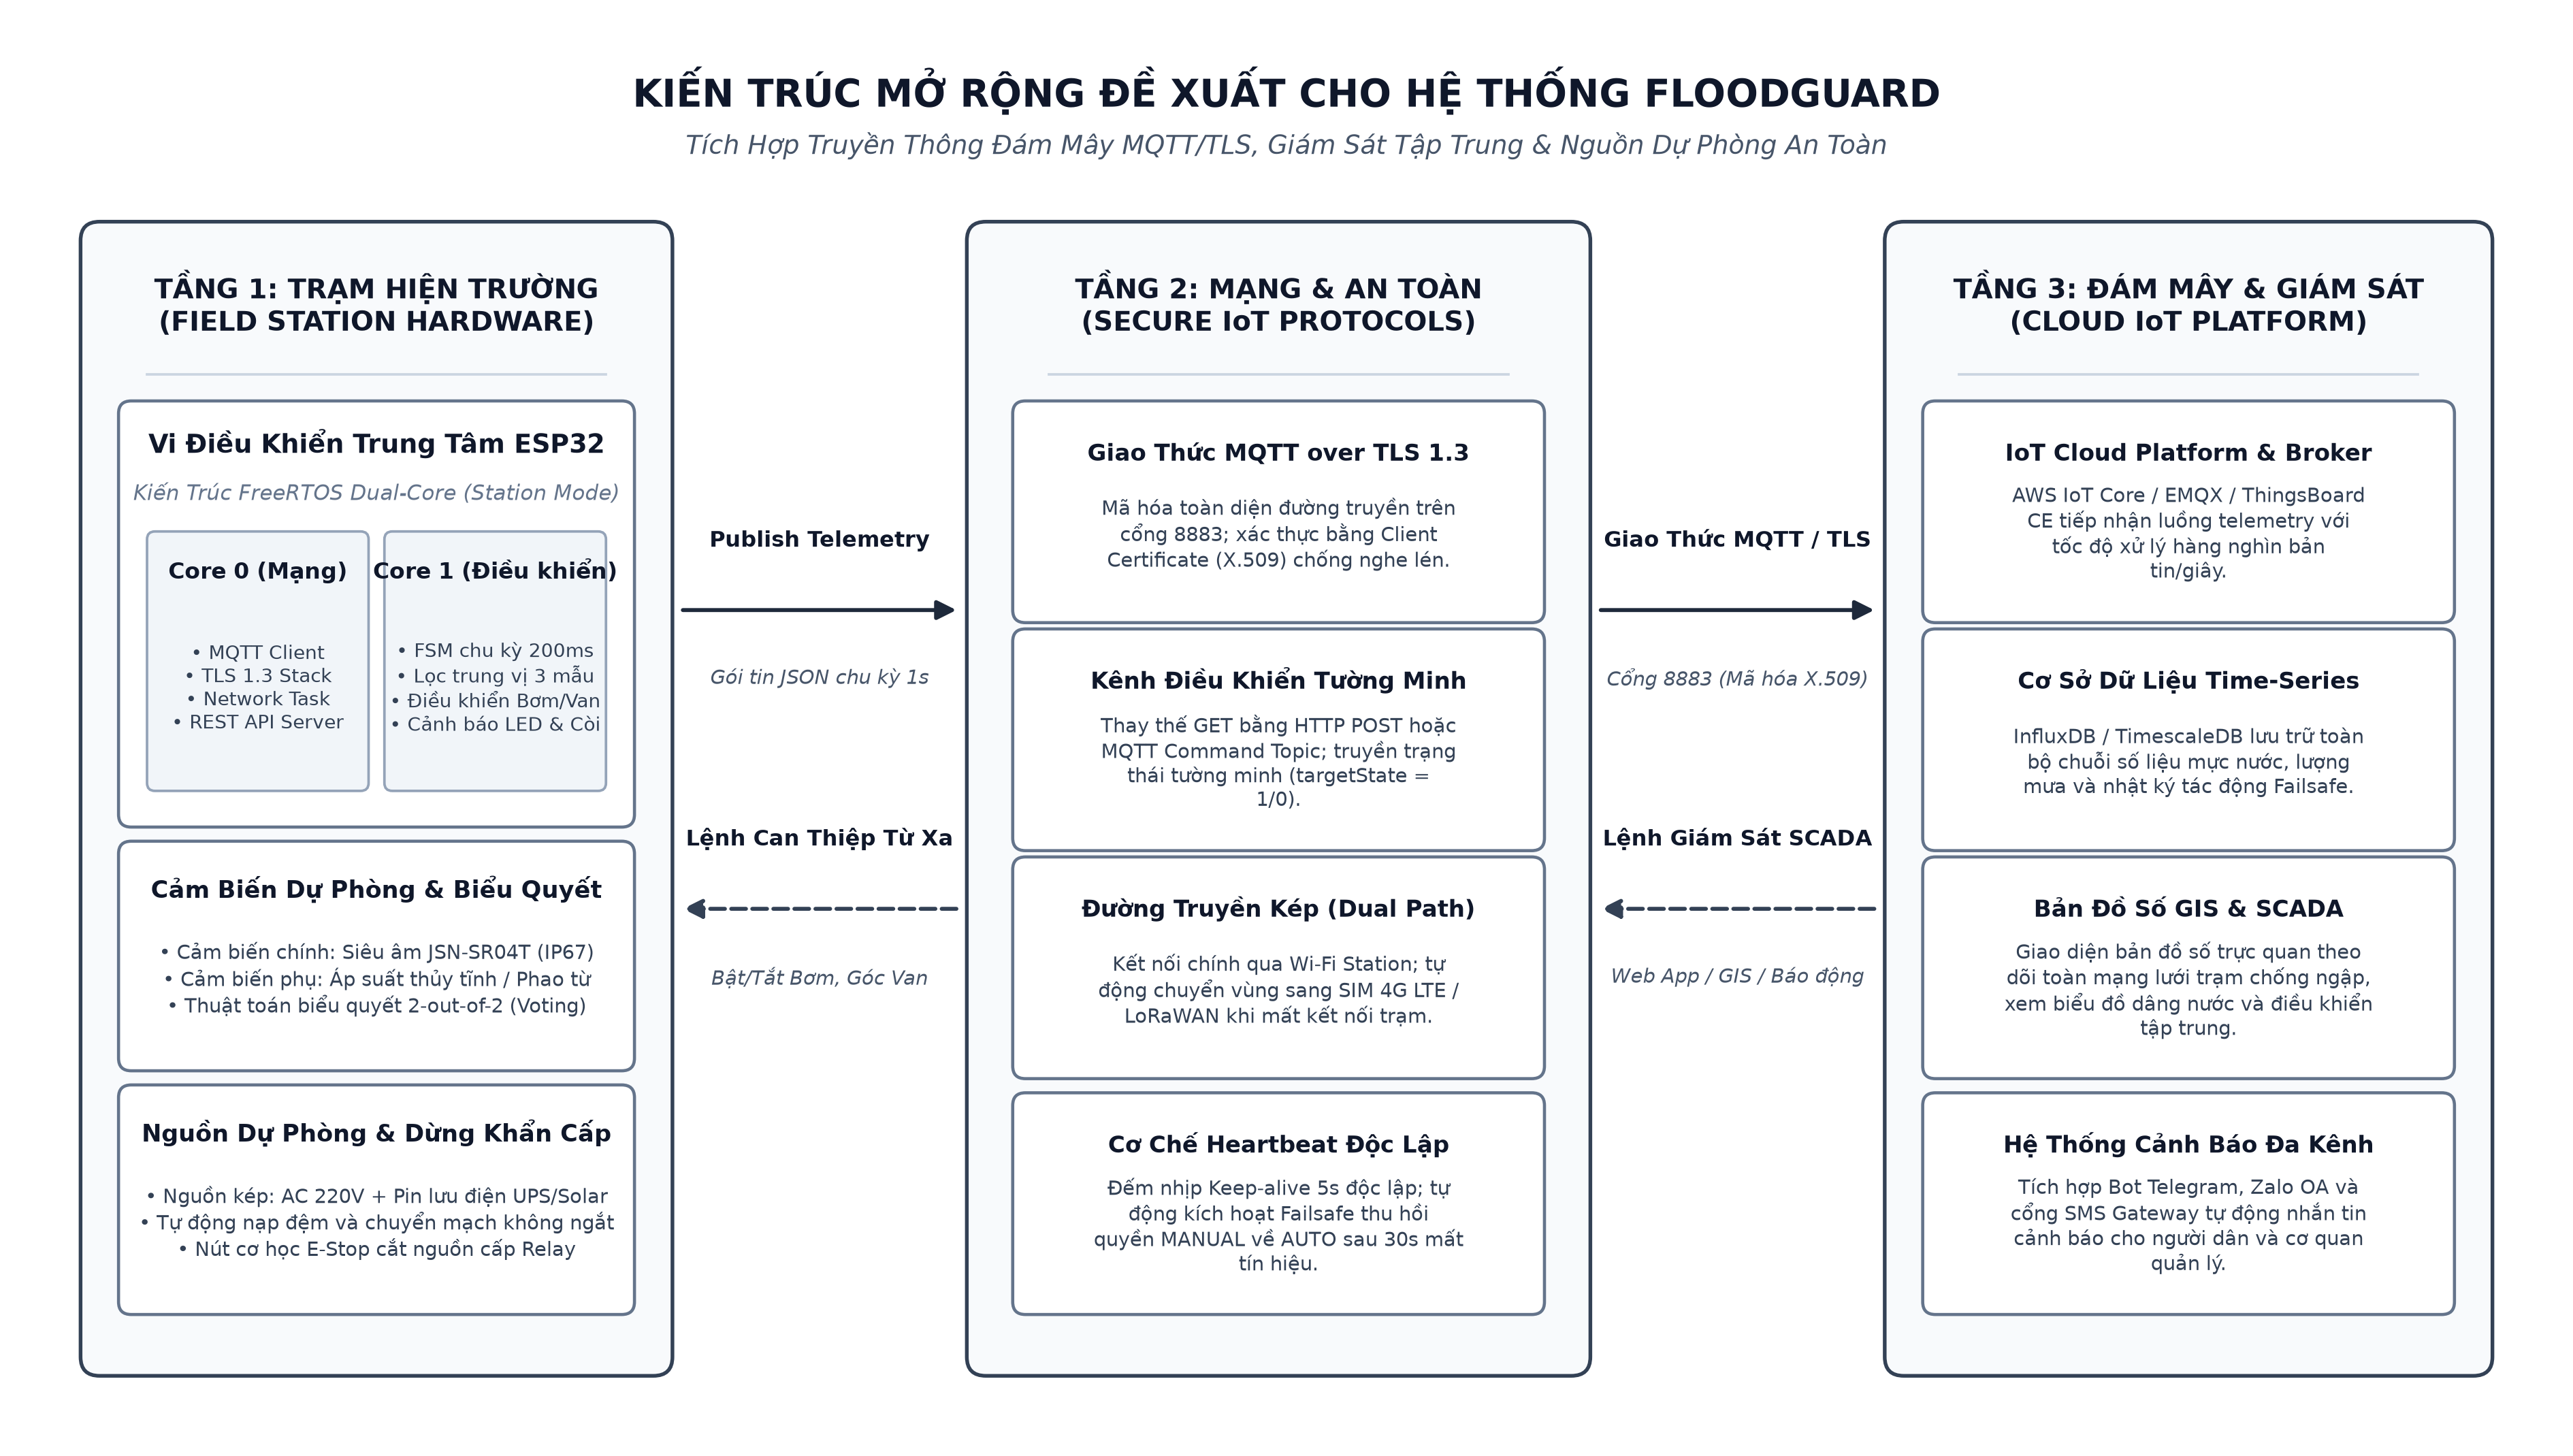
\includegraphics[width=0.98\textwidth]{figures/proposed_cloud_architecture.png}
    \caption{Kiến trúc mở rộng đề xuất cho hệ thống FloodGuard tích hợp Cloud IoT và nguồn dự phòng}
    \label{fig:cloud_architecture}
\end{figure}

\subsection{Định Hướng Dài Hạn}
Trong tầm nhìn dài hạn, giải pháp FloodGuard hướng tới mục tiêu trở thành một hệ thống phân tán thông minh trên quy mô đô thị:
\begin{enumerate}
    \item \textbf{Dự báo đỉnh ngập lụt bằng Trí tuệ nhân tạo biên (TinyML):} Huấn luyện và nén mô hình học máy nhẹ (mạng nơ-ron hồi quy LSTM hoặc mạng nơ-ron tích chập 1D) để nhúng trực tiếp vào vi điều khiển ESP32 sử dụng khung phần mềm \textbf{TensorFlow Lite for Microcontrollers}. Hệ thống sử dụng chuỗi dữ liệu thời gian thực của mực nước và lượng mưa để tự động dự báo trước đỉnh triều cường và nguy cơ tràn bờ trước từ $1 - 2\,\text{giờ}$, giúp chủ động kích hoạt hệ thống bơm hạ mực nước trước khi bão đổ bộ.
    \item \textbf{Mạng lưới quan trắc ngập lụt diện rộng (LoRaWAN Mesh):} Triển khai mạng lưới liên kết hàng chục trạm quan trắc dã chiến đặt rải rác dọc theo toàn bộ lưu vực sông ngòi, cống thoát nước và các điểm đen ngập úng đô thị thông qua công nghệ truyền thông vô tuyến tầm xa \textbf{LoRaWAN} ($868 / 915\,\text{MHz}$) với cự ly liên lạc từ $3 - 10\,\text{km}$, đảm bảo duy trì truyền số liệu ngay cả khi mạng viễn thông di động bị tê liệt hoàn toàn.
    \item \textbf{Tích hợp nền tảng bản đồ số GIS \& Đô thị thông minh:} Toàn bộ số liệu từ mạng lưới trạm được tích hợp lên bản đồ số không gian địa lý GIS của trung tâm điều hành đô thị thông minh (Smart City Operations Center), tự động đề xuất lộ trình giao thông an toàn tránh ngập lụt cho người dân trên ứng dụng di động công cộng.
    \item \textbf{Thương mại hóa \& Chứng nhận chuẩn an toàn công nghiệp:} Thiết kế lại toàn bộ mạch in PCB chuyên nghiệp theo tiêu chuẩn công nghiệp (chống nhiễu điện từ EMC/EMI, cách ly quang toàn phần, phủ lớp bảo vệ chống ẩm nhiệt đới Conformal Coating); tiến hành thử nghiệm nghiệm thu ngoài thực địa tại các trạm bơm tiêu đô thị thực tế.
\end{enumerate}

\section{Kết Luận Tổng Thể}
Đề tài \textbf{FloodGuard - Hệ thống giám sát và chống ngập thông minh} đã hoàn thành đầy đủ, trọn vẹn và vượt mức các mục tiêu kỹ thuật định lượng đã đề ra ban đầu. Dự án đã chứng minh tính khả thi, độ tin cậy và sự ưu việt của giải pháp kết hợp giữa vi điều khiển nhúng giá thành thấp ESP32, kiến trúc phần mềm thời gian thực phi chặn Super-Loop, thuật toán máy trạng thái hữu hạn FSM kết hợp dải trễ Hysteresis và giao diện Web Dashboard trực quan Dark Glassmorphism.

Hệ thống đã giải quyết triệt để hai bài toán cốt lõi trong kỹ thuật điều khiển trạm tiêu thoát nước: (1) Loại bỏ hoàn toàn hiện tượng rung giật đóng/ngắt thiết bị chấp hành khi mực nước dao động, bảo vệ an toàn cho cơ cấu cơ điện; (2) Thiết lập cơ chế tự trị Failsafe độc lập, đảm bảo trạm luôn vận hành an toàn tuyệt đối ngay cả khi mất liên lạc mạng điều khiển từ xa.

Mặc dù vẫn còn những hạn chế nhất định về quy mô mô hình sa bàn thí nghiệm và tính đơn sơ của giao thức mạng nội bộ, các bài học kinh nghiệm và lộ trình phát triển ba giai đoạn đã được xác lập một cách cụ thể, rõ ràng và có tính khả thi cao. Kết quả nghiên cứu của đề tài là nền tảng kỹ thuật vững chắc để tiếp tục phát triển, nâng cấp thành các sản phẩm thương mại hóa ứng dụng rộng rãi trong các dự án quan trắc môi trường và hạ tầng đô thị thông minh tại Việt Nam.


\end{document}
